% !TEX options=--shell-escape

%%%%%%%%%%%%%%%%%%%%%%%%%%%%%%%%%%%%%%%%%%%%%%%%%%%%%%%%%%%%%%%%%
%                                                               
%       User guide for the HPP observatory                           
%                                         
%                                                               
%       Andreas Bazzon                                          
%       Version 1.0                                             
%       February 2014
%
%       Natalia Engler
%       Version 1.1
%       November 2016
%
%       Luca Tortorelli
%       Version 2.0
%       November 2019  
%
%       Thomas Birbacher
%       Version 3.0
%       2023
%
%       Nicolas Feuchthoften & Alexander Liemen
%       Version 3.1
%       2023
%                                                               
%%%%%%%%%%%%%%%%%%%%%%%%%%%%%%%%%%%%%%%%%%%%%%%%%%%%%%%%%%%%%%%%%

\documentclass[a4paper, 11pt, fleqn]{memoir}

\usepackage{textcase}
\usepackage{fontspec}
\usepackage{microtype}
\usepackage[fleqn]{mathtools} % also loads amsmath
\usepackage{amstext}
\usepackage{unicode-math}
\usepackage{booktabs}

% (OPTIONAL) TO USE NICER FONTS, UNCOMMENT THE FOLLOWING:
% (You first have to download the following fonts and install them on your system: Libertinus, Libertinus Math, and Iosevka)

% UNCOMMENT BEGINS HERE

\defaultfontfeatures{Scale=MatchLowercase,
    Mapping=tex-text}
\setmainfont[Mapping=tex-text, % E.g. -- -> en-dash
    RawFeature={
            +onum;
        },
]{Libertinus Serif}
\setmonofont{Iosevka Term}
\setmathfont[math-style=ISO, bold-style=ISO]{Libertinus Math} %

% UNCOMMENT ENDS HERE

\usepackage{marginnote}
\NewDocumentCommand\trule{O{0.4pt}O{0pt}}{
\vskip0pt\vtop to0pt{
        \noindent\raisebox{#2}{\vbox{\leavevmode\hrule height#1}}}
}

\setsecnumdepth{subsection}
\settocdepth{section}

\makechapterstyle{Bringhurst}{%
    % \makechapterstyle{default}{%
    \chapterstyle{default}
    \setsecnumdepth{subsection}
    \renewcommand{\chaptitlefont}
    {\normalfont\bfseries%
        \addfontfeature{UprightFeatures={LetterSpace=6.0}}
    }
    \renewcommand{\chapnumfont}{%
        \fontspec[Numbers=OldStyle]{Libertinus Serif Display}
        \fontsize{72pt}{72pt}\selectfont
        \color{black}}
    \renewcommand*{\chapterheadstart}{}
    \renewcommand*{\printchaptername}{}
    \renewcommand*{\chapternamenum}{}
    % \renewcommand*{\printchapternum}{%
    %   \marginnote{\chapnumfont \thechapter}
    % }%
    \renewcommand*{\afterchapternum}{}
    \renewcommand*{\printchaptertitle}[1]{
        \chaptitlefont\raggedright\Huge\MakeUppercase{##1}}
    % \renewcommand*{\afterchaptertitle}{\trule\vspace{\baselineskip}}
    % \renewcommand*{\afterchaptertitle}{\baselineskip}

    \setsecindent{0pt}
    \setsecheadstyle{\normalfont\LARGE\bfseries\raggedright}

    \setsubsecindent{0pt}
    \setsubsecheadstyle{\normalfont\Large\bfseries\raggedright}

    \setsubsubsecheadstyle{\normalfont\large\bfseries\scshape\raggedright\MakeLowercase}

    \setparaheadstyle{\normalfont\raggedright\bfseries}
}

\usepackage[
    per-mode = symbol,
    exponent-product = \cdot
]{siunitx}

\DeclareSIUnit\electron{e^{-1}}
\DeclareSIUnit\pixel{px}
\DeclareSIUnit{\arcsecond}{\text{arcsec}}
\DeclareSIUnit{\arcminute}{\text{arcmin}}
\DeclareSIUnit{\adu}{\textsc{adu}}
\DeclareSIUnit{\parsec}{\text{pc}}
\DeclareSIUnit{\angstrom}{\text{Å}}
\DeclareSIUnit{\erg}{\text{erg}}

\usepackage{xparse}

\usepackage{csquotes}   % quotation marks
\usepackage{polyglossia}
\setdefaultlanguage{english}

\usepackage[version=4]{mhchem}

\usepackage{tabulary}
\usepackage{makecell} % forced line breaks in tables

\usepackage{xcolor}
\usepackage{graphicx}
\graphicspath{{figures/}}
\usepackage{caption}
\usepackage{subcaption}
\captionsetup{font=footnotesize, labelfont=bf}
\captionsetup[sub]{font=footnotesize}
\captionsetup{width=0.95\textwidth}
\captionsetup[sub]{width=0.95\textwidth}

% shaded boxes
\definecolor{oneblue}{RGB}{0,100,203}
\definecolor{darkblue}{RGB}{0,90,180}
\usepackage{mdframed}
\newmdenv[
    skipabove=7pt,
    skipbelow=7pt,
    rightline=false,
    leftline=true,
    topline=false,
    bottomline=false,
    linecolor=oneblue,
    backgroundcolor=oneblue!5,
    innerleftmargin=10pt,
    innerrightmargin=5pt,
    innertopmargin=5pt,
    leftmargin=0cm,
    rightmargin=0cm,
    linewidth=4pt,
    innerbottommargin=5pt
]{propBox}

\newenvironment{important}{
    \begin{propBox}
        %
        \textcolor{oneblue}{\textbf{\textit{Important.}}}
        }{
    \end{propBox}
}

\usepackage{enumitem}
\setlist*[enumerate]{noitemsep}
\setlist*[itemize]{noitemsep}

%
%   Code listings
%
\usepackage{listings}
\usepackage{lstautogobble}  % Fix relative indenting
\definecolor{bluekeywords}{rgb}{0.13, 0.13, 1}
\definecolor{greencomments}{rgb}{0, 0.5, 0}
\definecolor{redstrings}{rgb}{0.9, 0, 0}
\definecolor{graynumbers}{rgb}{0.5, 0.5, 0.5}
\lstset{
    autogobble,
    columns=fullflexible,
    showspaces=false,
    showtabs=false,
    breaklines=true,
    showstringspaces=false,
    breakatwhitespace=true,
    escapeinside={(*@}{@*)},
    commentstyle=\color{greencomments},
    keywordstyle=\color{bluekeywords},
    stringstyle=\color{redstrings},
    numberstyle=\color{graynumbers},
    basicstyle=\ttfamily\footnotesize,
    frame=l,
    framesep=12pt,
    xleftmargin=12pt,
    tabsize=4,
    captionpos=b
}
\usepackage[]{minted}

\setminted{
    autogobble,
    showspaces=false,
    showtabs=false,
    breaklines=true,
    escapeinside={(*@}{@*)},
    fontsize=\normalsize,
    xleftmargin=12pt,
    tabsize=4,
}

\usemintedstyle{manni}

\usepackage{float}
\usepackage{longtable}
\usepackage{floatflt}
\usepackage{wrapfig}

% BIBLIOGRAPHY
%
\usepackage[%
    autocite    = superscript,
    backend     = bibtex,
    sortcites   = true,
    isbn = false,
    url=false,
    abbreviate=true,
    date=year,
    eprint=false,
    style       = numeric-comp,
    doi=true,
]{biblatex}

\renewcommand*{\bibfont}{\normalfont}
\renewcommand{\UrlFont}{\ttfamily}

\makeatletter
\newcommand*{\blx@fnpct@movefor}{}
\newcommand*{\DeclareFootnoteMovePunct}{%
    \@ifstar
    {\let\blx@fnpct@movefor\@empty}
    {}
    \blx@def@fnpct@movefor}
\newcommand*{\blx@def@fnpct@movefor}{%
    \def\do##1{\blx@thecheckpunct{\listadd{\blx@fnpct@movefor}}##1}%
    \docsvlist}

\DeclareFootnoteMovePunct{.,{,}}

\newlength{\blx@fnpct@movelength}
\newcommand*{\blx@fnpct@footnotemover}[1]{%
    #1%
    \ifinlist{#1}{\blx@fnpct@movefor}
    {\settowidth{\blx@fnpct@movelength}{#1}%
        \hspace{-.8\blx@fnpct@movelength}}
    {}%
}

\protected\csedef{blx@acitei@superscript}#1#2#3#4#5{%
    \begingroup
    \blx@citeinit
    \noexpand\blx@fnpct@footnotemover{#5}%
    \blxcitecmd{supercite#1}{#2}{#3}{#4}{}%
    \endgroup}%
\protected\csedef{blx@macitei@superscript}#1#2#3{%
    \noexpand\blx@fnpct@footnotemover{#3}%
    #1{#2}%
    \endgroup}
\makeatother

\usepackage[perpage]{footmisc} % reset footnote counter per page

\usepackage[
    colorlinks=true,
    linkcolor=black,
    citecolor=blue,
    urlcolor=blue,
]{hyperref}
\usepackage[english, capitalize]{cleveref}
\DefineBibliographyStrings{english}{%
    urlseen={Accessed:}%
}
\addbibresource{bibliography.bib}
\DeclareFieldFormat{labelnumberwidth}{\mkbibbold{#1\adddot}}
% \crefformat{equation}{(#2#1#3)}

\renewcommand*{\thefootnote}{\fnsymbol{footnote}}

\begin{document}
\chapterstyle{Bringhurst}

\date{\today}
\author{Thomas Birbacher \and Luca Tortorelli}
\title{HPP Observatory \\ User Guide, Data Reduction and Experiments}

% \maketitle

\begin{titlingpage}
    \begin{center}
        \vspace{4cm}
        {\large\bfseries
        \begin{tabular}{ccc}
            Andreas Bazzon & Thomas Birbacher & Natalia Engler\\
            Nicolas Feuchthofen & Alexander Liemen & Luca Tortorelli
        \end{tabular}
        }\\
        \vspace{3cm}
        {\scalebox{1.8}{\Huge\bfseries \addfontfeature{LetterSpace=2.0} HPP TELESCOPE}}\\
        \vspace{0.6cm}
        {\LARGE\bfseries \addfontfeature{LetterSpace=2.0} USER MANUAL}\\
        \vfill
        
\includegraphics{eth-logo}\\
        Version 3.2\\
        \today
    \end{center}
\end{titlingpage}

\newcommand{\software}[1]{\texttt{#1}}

\frontmatter

\chapter{Overview}

\subsection*{Purpose of this manual}

This manual shows the procedures for starting, operating, and shutting down the \textsc{hpp} telescope, which is mostly intended for students and outreach activities.
The manual also contains a list of possible experiments and a guide to data reduction.

\subsection*{Contact \& source code}

Current contact for the telescope: \url{thomabir@phys.ethz.ch}

\noindent Current version of this manual \& LaTex source code: \url{https://github.com/thomabir/hpp-telescope-manual}

\cleardoublepage

\tableofcontents

\mainmatter

\part{Observatory Operation}

\chapter{General}

\section{List of equipment}

\begin{itemize}
    \item Telescope: Planewave \textsc{cdk20}, see \cref{tab:specs-telescope} for details.
    \item Mount: 10micron \textsc{gm4000hps}, see \cref{tab:specs-mount} for details.
    \item Camera: The camera is a \textsc{sbig stx-16803} \textsc{ccd}, see \cref{tab:specs-camera} for details.
\end{itemize}

\begin{table}[h!]
    \centering
    \begin{tabular}{ll}
        \toprule
        \multicolumn{2}{c}{\textbf{Planewave \textsc{cdk20} telescope}}                                         \\
        \midrule
        Optical design                                 & Corrected Dall-Kirkham                                 \\
        Aperture diameter                              & $\num{20}\,\text{in} = \SI{508}{\mm}$                  \\
        \phantom{Aperture} area                        & \SI{0.203}{\m\squared}                                 \\
        Focal length                                   & \SI{3454}{\mm}                                         \\
        Diffraction limit at $\lambda = \SI{500}{\nm}$ & \SI{0.25}{\arcsecond}                                  \\
        Focal ratio                                    & $ f/\num{6.8}$                                         \\
        Central obstruction diameter                   & $\SI{39}{\percent} \equiv \SI{19.8}{\cm}$              \\
        \phantom{Central obstruction} area             & $\SI{15}{\percent} \equiv \SI{308}{\cm\squared}$       \\
        Backfocus from racked-in focuser               & \SI{147}{\mm}                                          \\
        \midrule
        \multicolumn{2}{c}{Telescope + imaging chip}                                                            \\
        \midrule
        Field of view                                  & $\num{36.7} \times \num{36.7}$ \si{\arcminute\squared} \\
        Diagonal field of view                         & \SI{51.9}{\arcminute}                                  \\
        Plate scale                                    & \SI{0.537}{\arcsecond\per\pixel}                       \\
        \midrule
        \multicolumn{2}{c}{Telescope + guiding chip}                                                            \\
        \midrule
        Field of view                                  & $\num{4.71} \times \num{3.54}$\si{\arcminute\squared}  \\
        Diagonal field of view                         & \SI{5.89}{\arcminute}                                  \\
        Plate scale                                    & \SI{0.442}{\arcsecond\per\pixel}                       \\
        \bottomrule
    \end{tabular}
    \caption{Specifications of the telescope.}
    \label{tab:specs-telescope}
\end{table}

\begin{table}[h!]
    \centering
    \begin{tabular}{ll}
        \toprule
        \multicolumn{2}{c}{\textbf{10micron \textsc{gm4000hps} mount}}                           \\
        \midrule
        Type              & German equatorial mount                                              \\
        Encoder           & absolute, both axes, error $< \SI{0.1}{\arcsecond}$                  \\
        Pointing accuracy & $< \SI{20}{\arcsecond}$                                              \\
        Tracking accuarcy & $\approx \SI{1}{\arcsecond}$ peak-to-peak typ. over \SI{15}{\minute} \\
        \bottomrule
    \end{tabular}
    \caption{Specifications of the mount.}
    \label{tab:specs-mount}
\end{table}

\begin{table}[h!]
    \centering
    \begin{tabular}{ll}
        \toprule
        \multicolumn{2}{c}{\textbf{\textsc{Sbig stx-16803} camera}}                                                    \\
        \midrule
        \multicolumn{2}{c}{Imaging chip}                                                                               \\
        \midrule
        \textsc{Ccd} chip                 & Kodak KAF-16803                                                            \\
        Resolution                        & $\SI{4096}{\pixel} \times \SI{4096}{\pixel} = \SI{16.777216}{\mega\pixel}$ \\
        Pixel size                        & $\SI{9}{\um} \times \SI{9}{\um}$                                           \\
        \textsc{ccd} dimensions           & $\SI{36.864}{\mm} \times \SI{36.864}{\mm}$                                 \\
        \textsc{ccd} diagonal             & $\approx \SI{52.13}{\mm}$                                                  \\
        \midrule
        \multicolumn{2}{c}{Guiding chip}                                                                               \\
        \midrule
        \textsc{ccd} chip                 & Kodak KAI-340                                                              \\
        Resolution                        & $\SI{640}{\pixel} \times \SI{480}{\pixel}$                                 \\
        Pixel size                        & $\SI{7.4}{\um} \times \SI{7.4}{\um}$                                       \\
        \textsc{ccd} dimensions           & $\SI{4.736}{\mm} \times \SI{3.552}{\mm}$                                   \\
        \textsc{ccd} diagonal             & \SI{5.92}{\mm}                                                             \\
        Distance between guiding chip     &                                                                            \\
        and imaging chip                  & $\approx \SI{6}{\mm}$                                                      \\
        \midrule
        \multicolumn{2}{c}{Electronics}                                                                                \\
        \midrule
        Saturation signal                 & \num{65535}
        ADU                                                                                                            \\
        Quantum efficiency                & \SI{60}{\percent} at \SI{550}{\nm}                                         \\
        Read noise                        & \SI{9}{\electron} \textsc{rms}                                             \\
        Dark current                      & \SI{3}{\electron\per\pixel\per\second} at \SI{25}{\celsius},               \\
                                          & \SI{0.02}{\electron\per\pixel\per\second} at \SI{-20}{\celsius}            \\
        Dark current doubling temperature & \SI{6.3}{\celsius}                                                         \\
        A/D Gain                          & \SI{1.27}{\electron}/ADU                                                   \\
        A/D bits                          & \SI{16}{\bit}                                                              \\
        \midrule \multicolumn{2}{c}{Other}                                                                             \\
        \midrule Exposure time            & \SIrange{0.1}{3600}{\second}                                               \\
        Pixel digitisation rate           & \SI{1.8}{\mega\pixel\per\second}                                           \\
        Full frame digitisation time      & \SI{9.5}{\second}                                                          \\
        Full frame download time          & \SI{2}{\second}                                                            \\
        Cooling                           & Two stage thermoelectric, \SI{-50}{\celsius}$\Delta T$                     \\
        Power supply                      & \SI{12}{\volt} \textsc{dc} at \SI{9.5}{\ampere}                            \\
        \bottomrule
    \end{tabular}
    \caption{Specifications of the camera} \label{tab:specs-camera}
\end{table}

\clearpage

\section{Start-up} The following steps have to be performed to use the telescope:
\begin{enumerate}
    \item Open the dome
    \item Remove the mirror cover
    \item Power-on the instruments
    \item Unpark the mount
\end{enumerate}
They are described in detail in the next sections.

\subsection{Opening the dome}

Observations are only allowed if the dome can be opened completely and locked in its open position.
To open the dome, follow these steps:
\begin{enumerate}
    \item Fully open both doors.
    \item Snap the doors into their door locks such that they cannot swing back, as in \cref{fig:door-locks}.
    \item Release the dome locks located inside the dome, see \cref{fig:dome-locks}.
    \item Check that the telescope is correctly parked, and that it will fit past the doors.
    \item (During winter) Make sure that no snow or dirt can fall onto the telescope when opening the dome.
    \item From inside the dome, push the dome away from the telescope, until it has reached the open position.
          Check that the telescope fits through the door while pushing.
    \item Engage the dome locks.
    \item (Optional) Close the doors.
\end{enumerate}

\begin{figure}
    \centering
    \begin{subfigure}[c]{0.47\textwidth}
        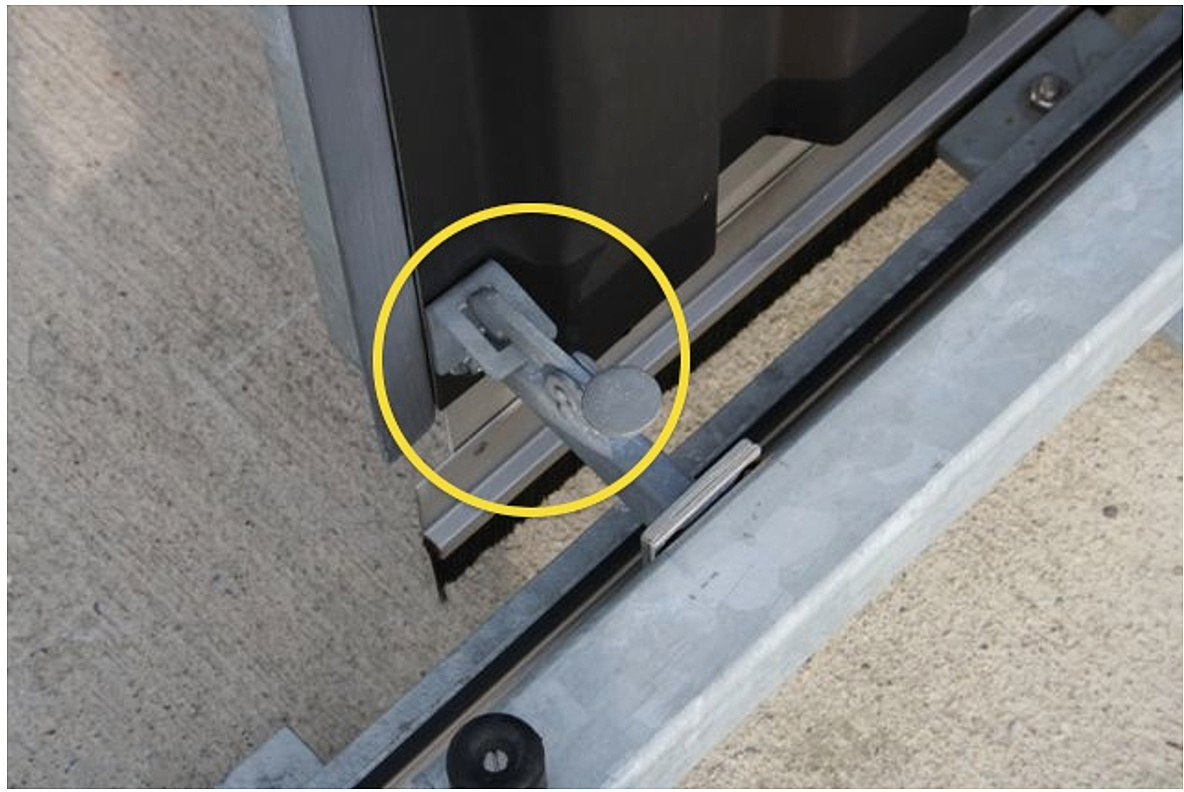
\includegraphics[width=\textwidth]{door_secure-locks}
        \subcaption{Door locks}
        \label{fig:door-locks}
    \end{subfigure}
    \begin{subfigure}[c]{0.47\textwidth}
        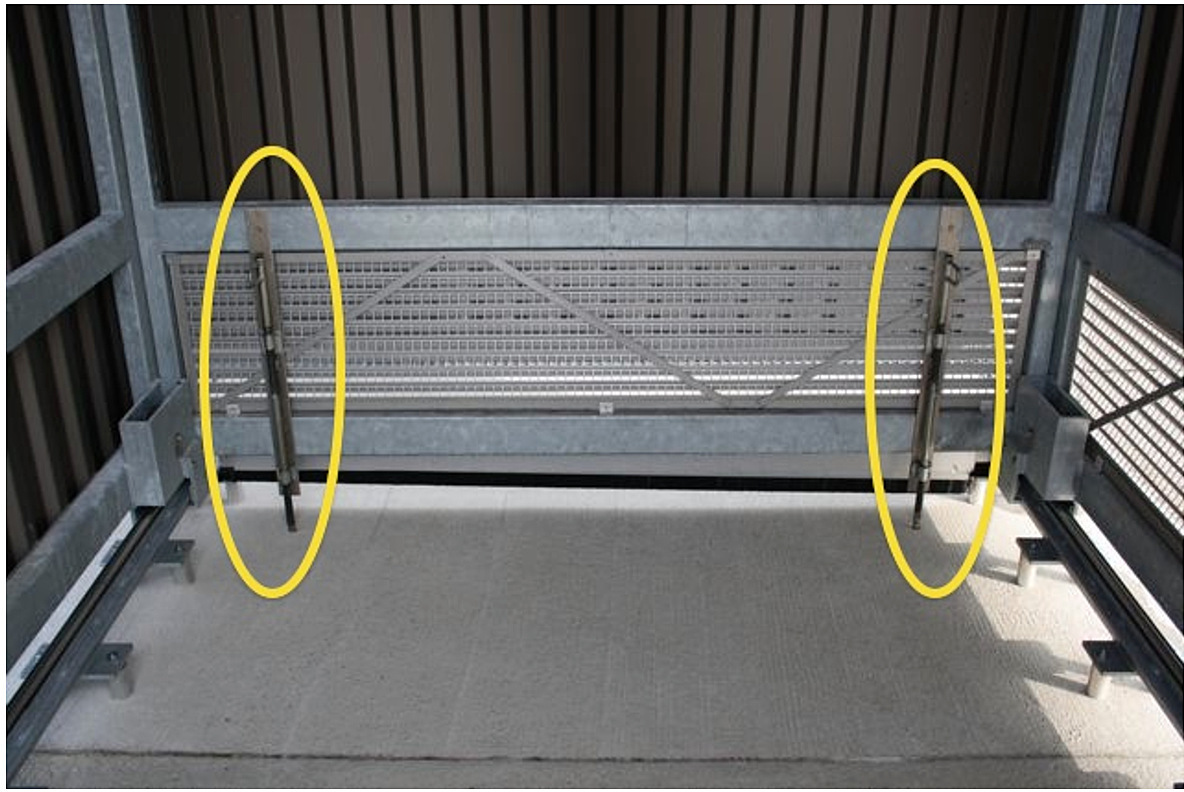
\includegraphics[width=\textwidth]{dome_secure-locks}
        \subcaption{Dome locks}
        \label{fig:dome-locks}
    \end{subfigure}
    \caption{Opening the dome}
\end{figure}

\subsection{Removing the mirror cover}
\label{sec:mirror-cover}

When the telescope is not in use, cover the primary mirror with the mirror cover, see \cref{fig:mirror-cover}.
To install or remove the cover, pull back the spandex stray light cover, and pass the mirror cover past the bars.

\begin{figure}
    \centering
    \begin{subfigure}[c]{0.47\textwidth}
        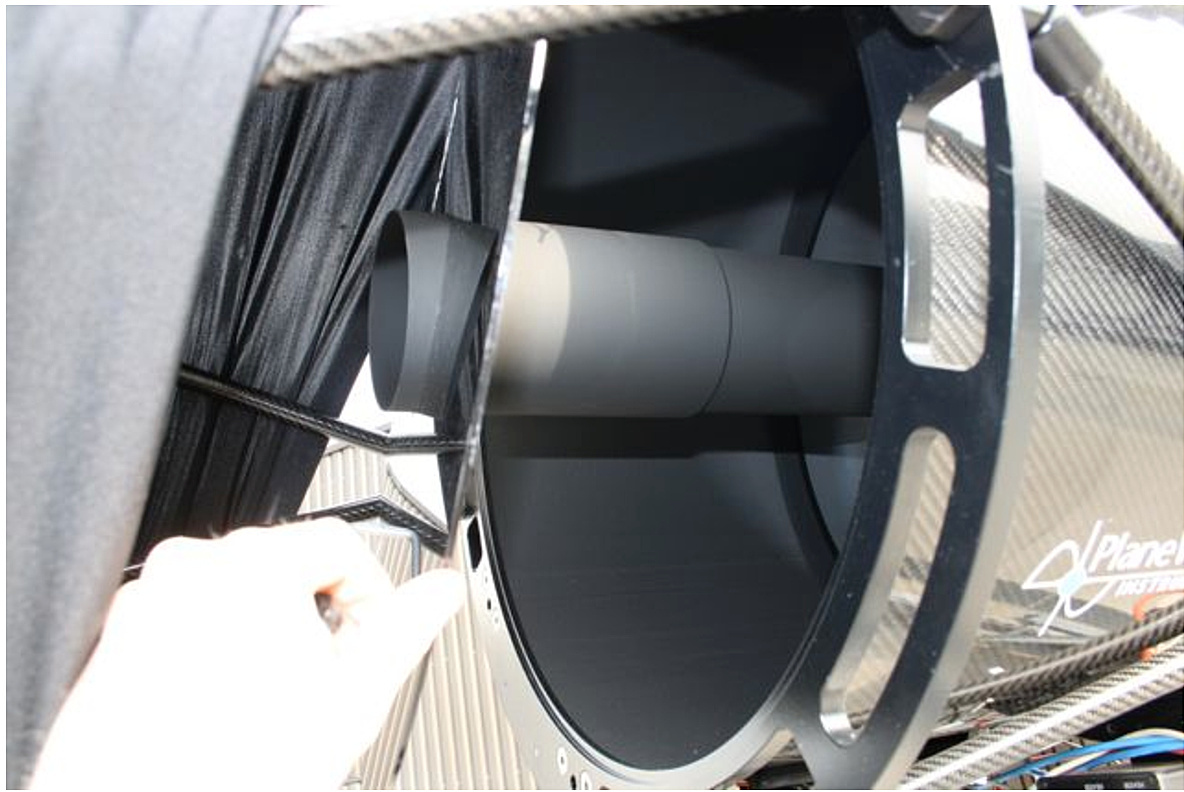
\includegraphics[width=\textwidth]{mirror-cover}
        \subcaption{Mirror cover.}
        \label{fig:mirror-cover}
    \end{subfigure}
    \begin{subfigure}[c]{0.47\textwidth}
        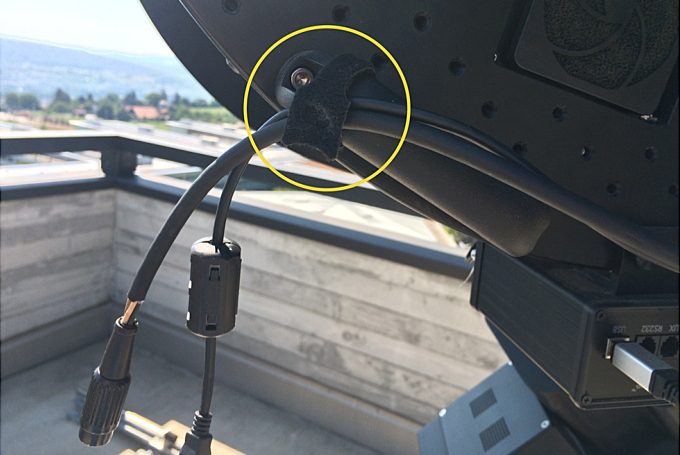
\includegraphics[width=\textwidth]{cable-strap}
        \caption{Strap to fix loose cables.}
        \label{fig:cable-strap}
    \end{subfigure}
    \caption{ }
\end{figure}

\subsection{Power-on the instruments}

To power on the instruments, perform the following actions:
\begin{enumerate}
    \item \textbf{Check instruments.
          }
          Check that all the instruments required for the observation are installed.
          In particular, check that the camera is installed.
          Follow \cref{sec:install-camera} to mount or unmount the camera.
    \item \textbf{Check cables.}
          Make sure that there are no cables hanging loose that could get stuck during telescope movement.
          Use the straps shown in \cref{fig:cable-strap} to fix them.
    \item \textbf{Power on the main power strip.}
          Press the main power switch on the bottom of the electronics tray (circle in \cref{fig:electronics-overview}).
          You should hear the camera fans starting up.
    \item \textbf{Power on the telescope computer.}
          On the back of the telescope computer (marked A in \cref{fig:electronics-overview}), press the power button, as shown in \cref{fig:telescope-pc-power-switch}.
          You should hear a beeping sound as the computer boots.
    \item \textbf{Power on the mount.}
          Push on the mount power button, shown in \cref{fig:mount-power-switch}, for half a second, then let go again.
          The button looks like a toggle switch, but it is not.
          It will spring back into its original position after releasing it.
    \item \textbf{Check the hand controller.}
          Confirm that the hand-controller of the mount lights up and boots.
          If this is not the case, repeat step 5 (maybe with a bit more pressure, or a bit shorter) until it boots.
          Booting takes approximately 30 seconds.
    \item (Optional) \textbf{Check time and date.}
          Check that the hand controller of the mount displays the correct time and date.
          Note that the mount is not really aware of daylight savings time / summer time, so an offset of exactly one hour in summer may be normal.
          If the mount believes it's 2012, you may have to change to mount battery, see \cref{sec:mount-battery-replace}.
\end{enumerate}

\begin{figure}[h!]
    \centering
    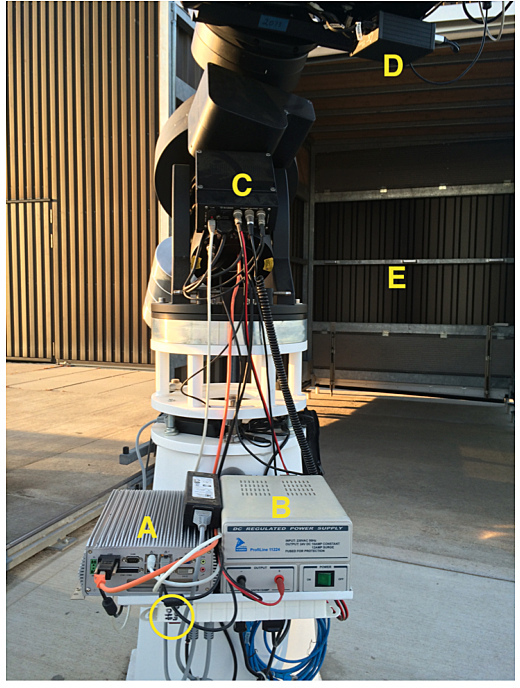
\includegraphics[width=0.47\textwidth]{electronics-overview}
    \caption{Overview of electronics: main power switch (circle), remote computer (A), mount power supply (B), mount control box (C), heater control box (D), handles to move dome (E).}
    \label{fig:electronics-overview}
\end{figure}

\begin{figure}
    \centering
    \begin{subfigure}[b]{0.47\textwidth}
        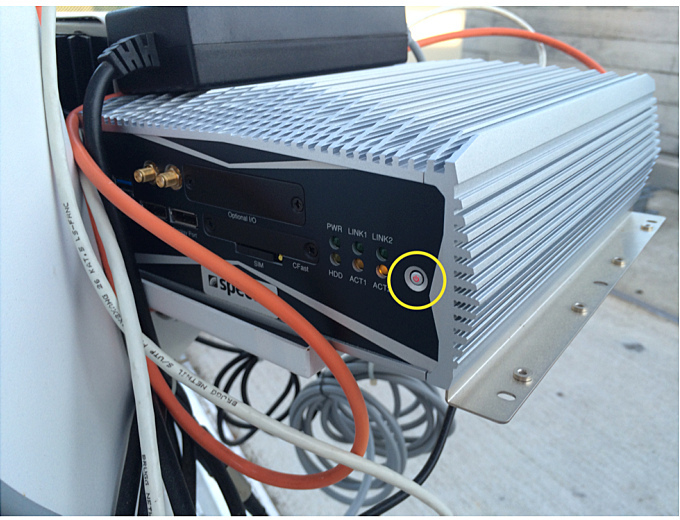
\includegraphics[width=\textwidth]{remotePC-switch}
        \caption{Power switch of the remote computer.}
        \label{fig:telescope-pc-power-switch}
    \end{subfigure}
    \begin{subfigure}[b]{0.47\textwidth}
        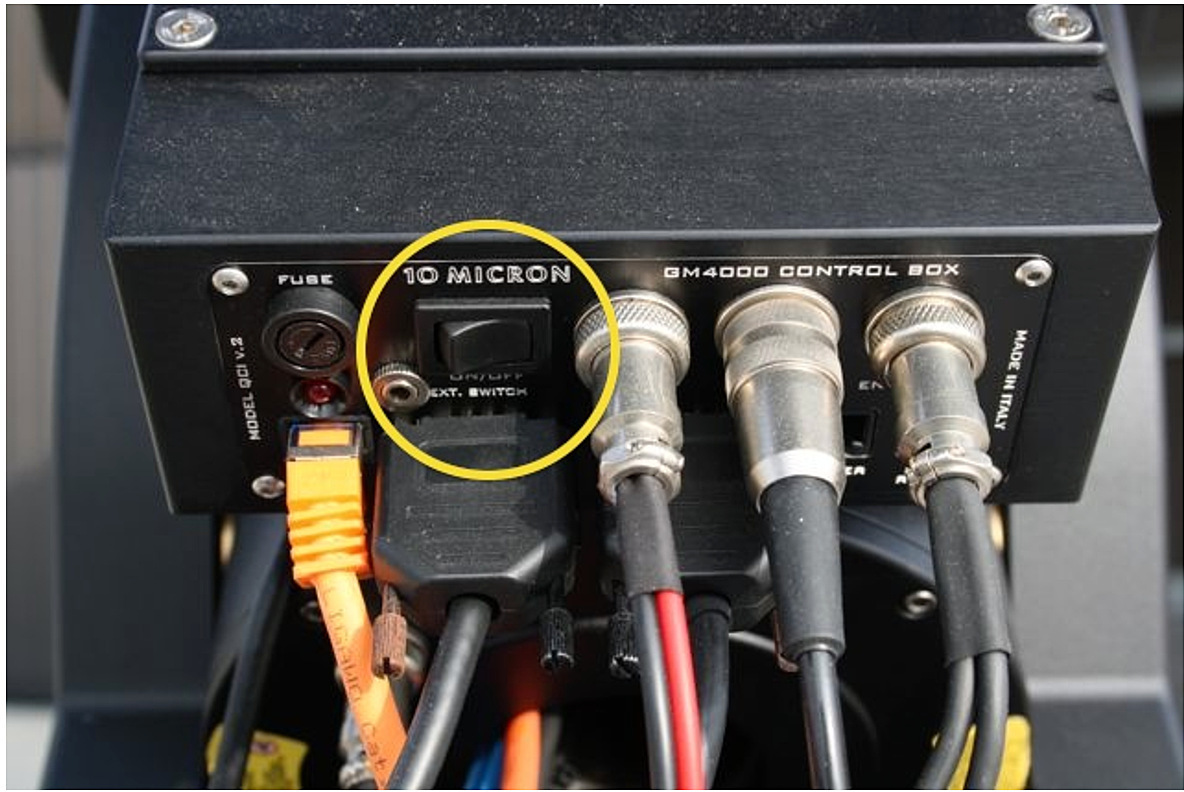
\includegraphics[width=\textwidth]{gm4000-control-box}
        \caption{Power button of the mount.}
        \label{fig:mount-power-switch}
    \end{subfigure}
    \caption{Power buttons}
\end{figure}

\subsection{Unparking the mount}
After the mount has booted, it will be in its parked position, where it cannot move.
The mount can be unparked from the control software or from the hand controller.
To unpark the mount with the hand controller, go to \texttt{Menu -> Alignment -> Unpark}.

\section{Shutdown}
\label{shutdown}

The shut-down procedure is the reverse of the start-up procedure:
\begin{enumerate}
    \item Park the mount, and wait until it has finished the parking procedure.
    \item Disconnect the control software (e.g.
          N.I.N.A., PWI3) using the remote computer.
    \item Shutdown the remote computer.
    \item (Optional, if you used the finder scope) Turn off the light of the finder scope.
    \item Shutdown the mount, and wait until the hand controller goes dark.
    \item Turn off the main power switch
    \item Install the mirror cover
    \item Open the dome doors and lock the doors in place
    \item Release the dome locks
    \item Pull the dome from the inside, while continuously checking that the telescope fits through the dome
    \item Engage the dome locks
    \item Close doors and lock them
\end{enumerate}

\section{Maintenance}

\subsection{Replacing the mount battery}
\label{sec:mount-battery-replace}

If the clock of the mount resets whenever you power off the mount, the battery of the controller is probably dead.
Open the connection box of the mount (where the controller plugs in), and replace the \textsc{cr3032} coin cell with a new one.
The battery should last for a few years.

To change the time with the hand controller: \texttt{MENU -> Local data -> Clock -> Date and time}.
You can also use the \texttt{Clock Sync} software on the computer.

\subsection{Finder scope}
The finder scope (\cref{fig:finder-scope}) has a holographic sight that can be used to roughly align the telescope.
It is currently not aligned with the main telescope.
After using it, do not forget to switch off the holographic sight, since the battery will run out otherwise.

\begin{figure}[t!]
    \centering
    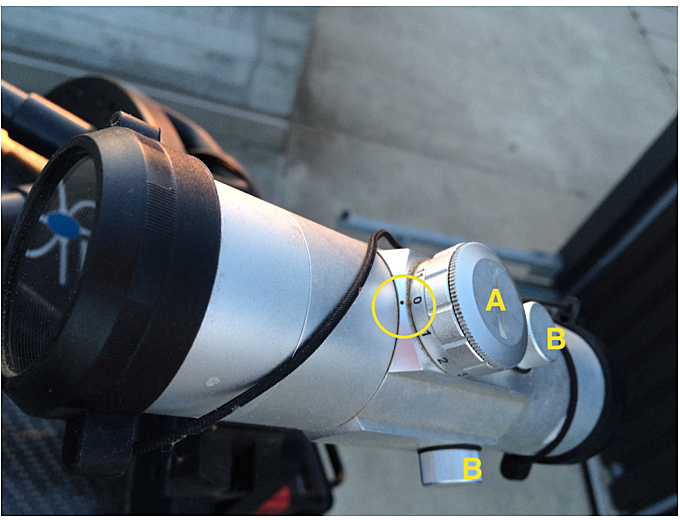
\includegraphics[width=0.47\textwidth]{finder-scope}
    \caption{Finder scope.
        Off position (circle) for the light modulator from the front.
        Also indicated are the caps (B) which protect the alignment knobs for x and y direction.
    }
    \label{fig:finder-scope}
\end{figure}

\subsection{Mounting the camera}
\label{sec:install-camera}

\begin{important}
    Mounting or dismounting the camera requires two people.
    Do not try it on your own!
\end{important}

To mount the camera, use the red US Allen key set.
\begin{enumerate}
    \item
          Remove the eyepiece and the eyepiece adapter plate from the telescope with a 5/32'' Allen key, see \cref{fig:adapter-plate-eyepiece}.
    \item
          Attach the camera adapter plate to the telescope with a 5/32'' Allen key, see \cref{fig:adapter-plate-camera}.
          Make sure the wedge in the adapter plate faces away from the CDK control panel.
    \item
          Remove the cover plate from the cover, see \cref{fig:camera-cover-plate}.
    \item
          Loosen the four screws at the camera flange with a 5/64'' Allen key, see \cref{fig:camera-mount-screws}.
    \item
          Bring the camera to the telescope.
          One person holds the camera such that the autoguider head is on the same side as the wedge in the adapter plate, see \cref{fig:camera-attach}.
    \item
          The other person fixes the four screws at the camera flange with a 5/64'' Allen key, see \cref{fig:camera-attach}
    \item
          Remove the camera USB and power cables from the cable strap.
    \item
          Plug in the power and USB cables, see \cref{fig:camera-cables}.
\end{enumerate}

\begin{figure}
    \centering
    \begin{subfigure}[t]{0.47\textwidth}
        \centering
        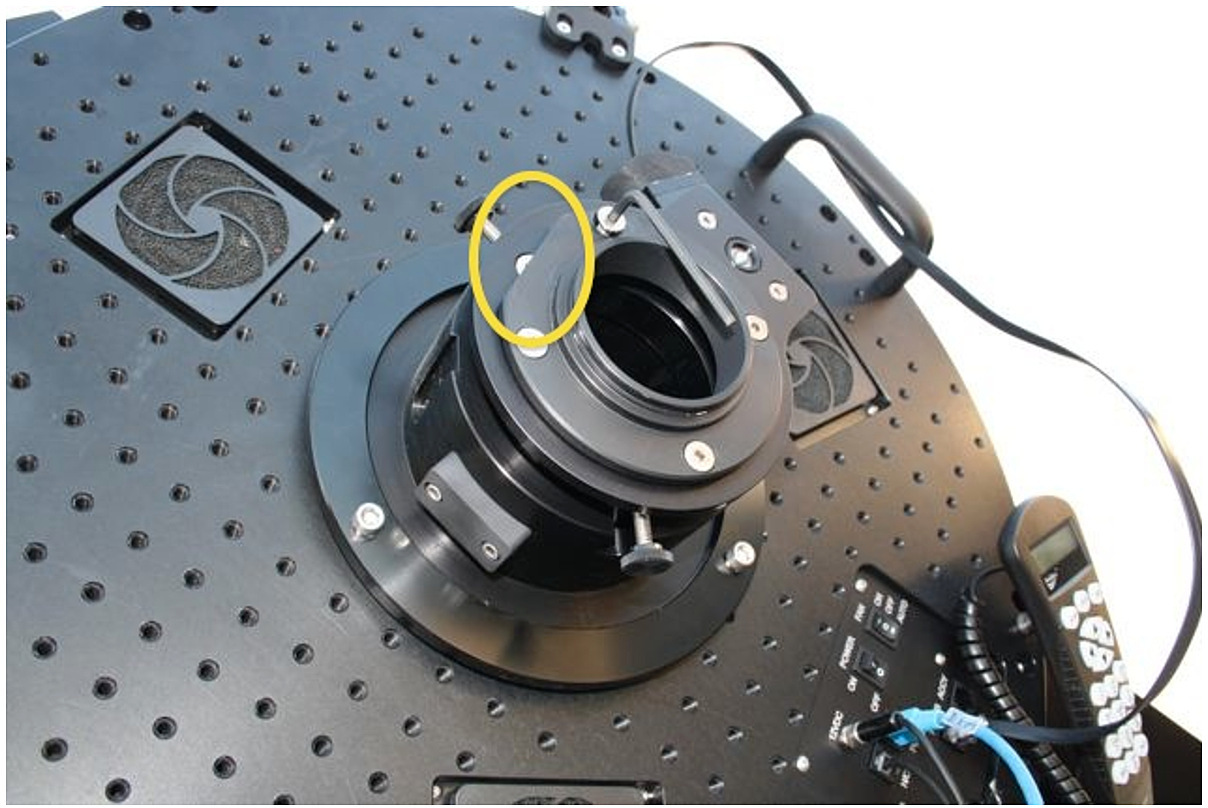
\includegraphics[width=\textwidth]{adapter-ccd}
        \caption{Adapter plate for the camera.
            Note that the wedge in the adapter plate, marked by a circle, must face up, away from the CDK control panel.
        }
        \label{fig:adapter-plate-camera}
    \end{subfigure}
    \begin{subfigure}[t]{0.47\textwidth}
        \centering
        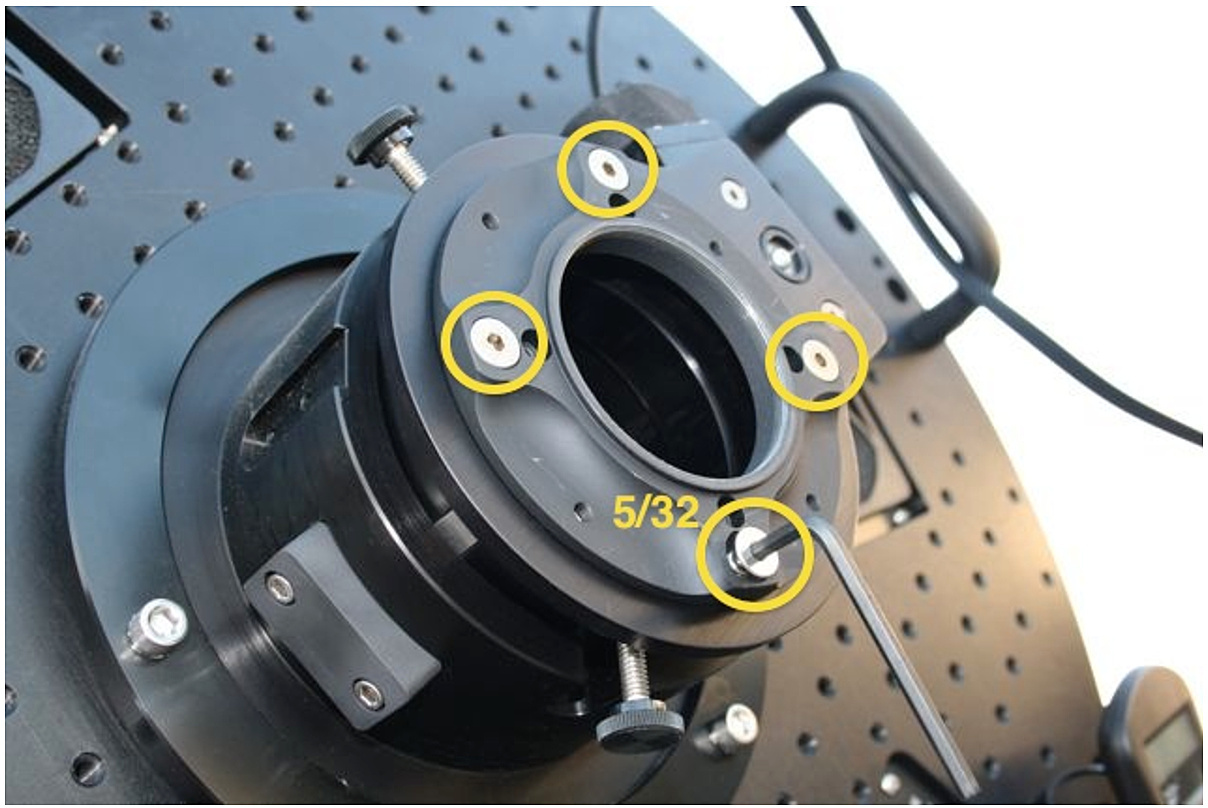
\includegraphics[width=\textwidth]{adapter-visual}
        \caption{Adapter plate for visual observations.}
        \label{fig:adapter-plate-eyepiece}
    \end{subfigure}
    \caption{Adapter plates for attaching equipment.
        Use a 5/32'' Allen key to change adapter plates.
    }
\end{figure}

\begin{figure}
    \centering
    \begin{subfigure}[t]{0.47\textwidth}
        \centering
        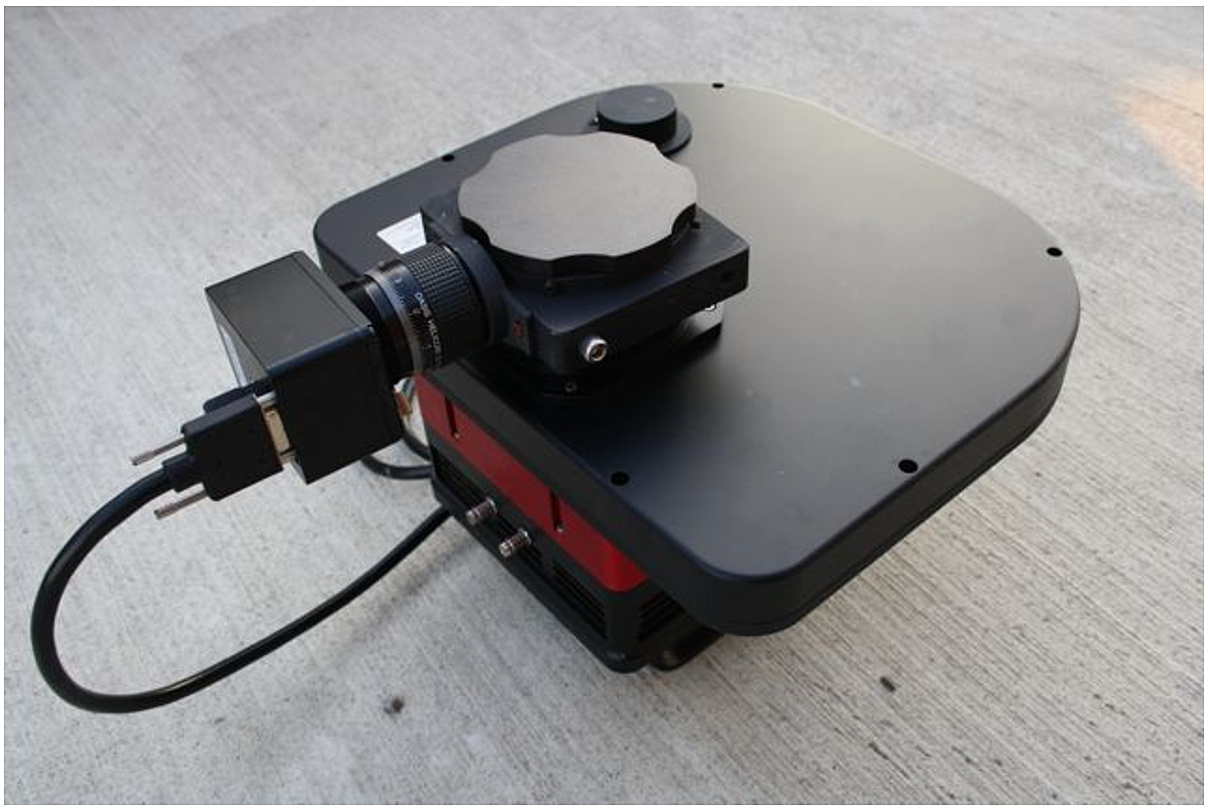
\includegraphics[width=\textwidth]{ccd-closed}
        \caption{The cover plate is attached for storage.}
        \label{fig:camera-cover-plate}
    \end{subfigure}
    \begin{subfigure}[t]{0.47\textwidth}
        \centering
        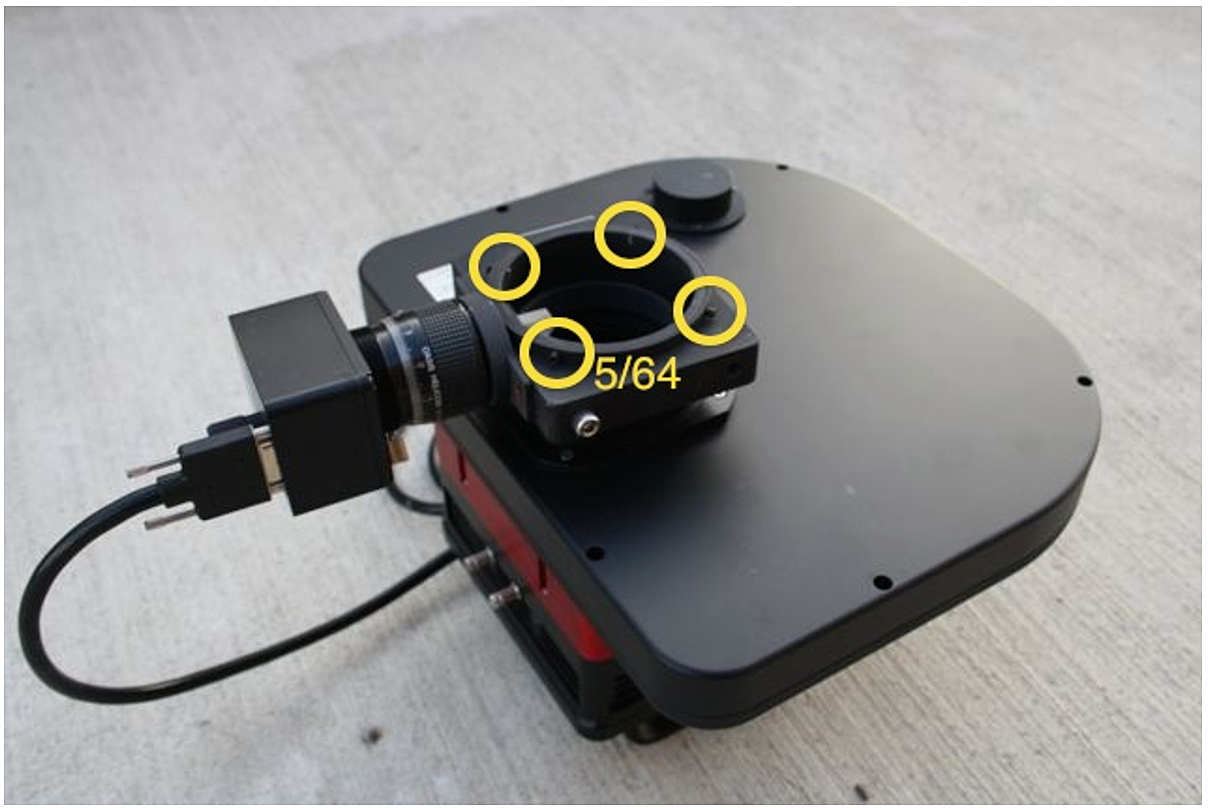
\includegraphics[width=\textwidth]{ccd-open}
        \caption{To mount the camera, loosen the four screws at the flange with a 5/64'' Allen key}
        \label{fig:camera-mount-screws}
    \end{subfigure}
    \caption{The camera in its storage configuration.}
\end{figure}

\begin{figure}
    \centering
    \begin{subfigure}[t]{0.45\textwidth}
        \centering
        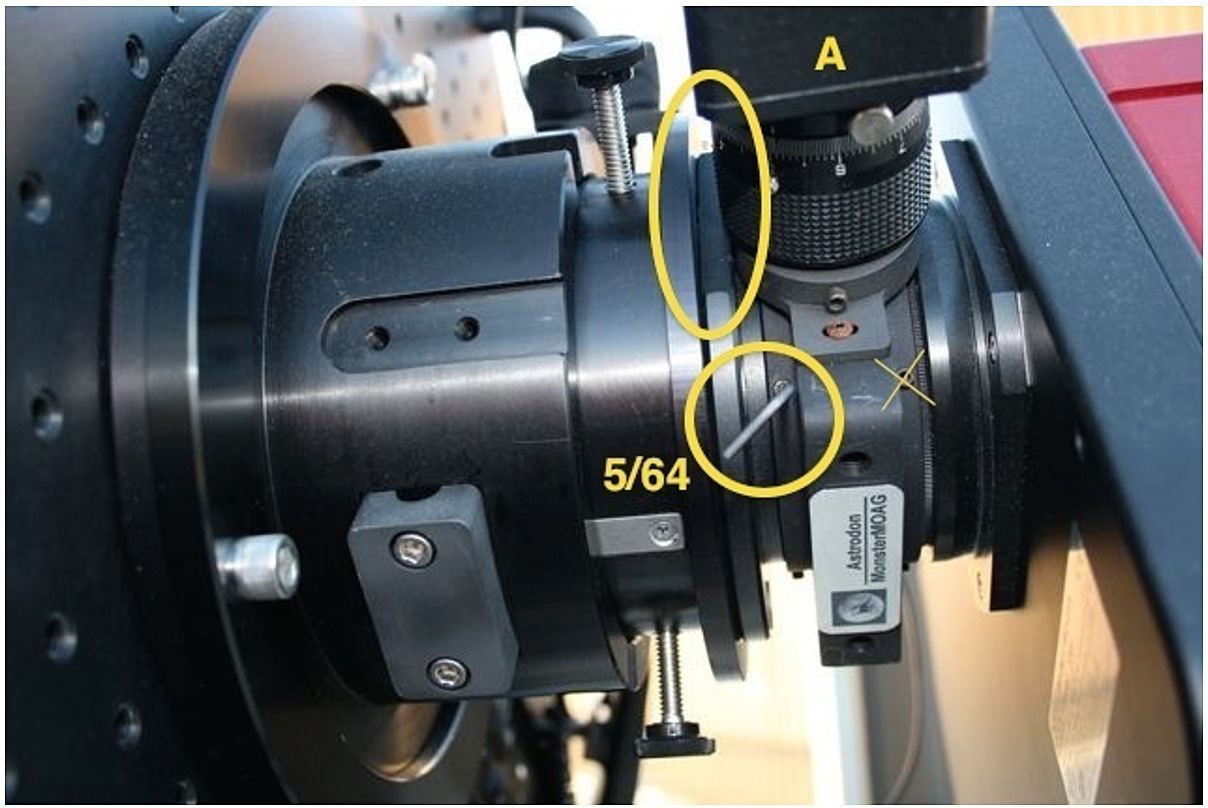
\includegraphics[width=\textwidth]{attach-ccd}
        \subcaption{Attaching the camera.
            Note that the autoguider head (A) is at the same side as the wedge of the adapter plate.
            Make sure the camera flange tightly fits to the camera adapter plate and then tighten all four screws with a 5/64'' Allen key.
        }
        \label{fig:camera-attach}
    \end{subfigure}
    \begin{subfigure}[t]{0.45\textwidth}
        \centering
        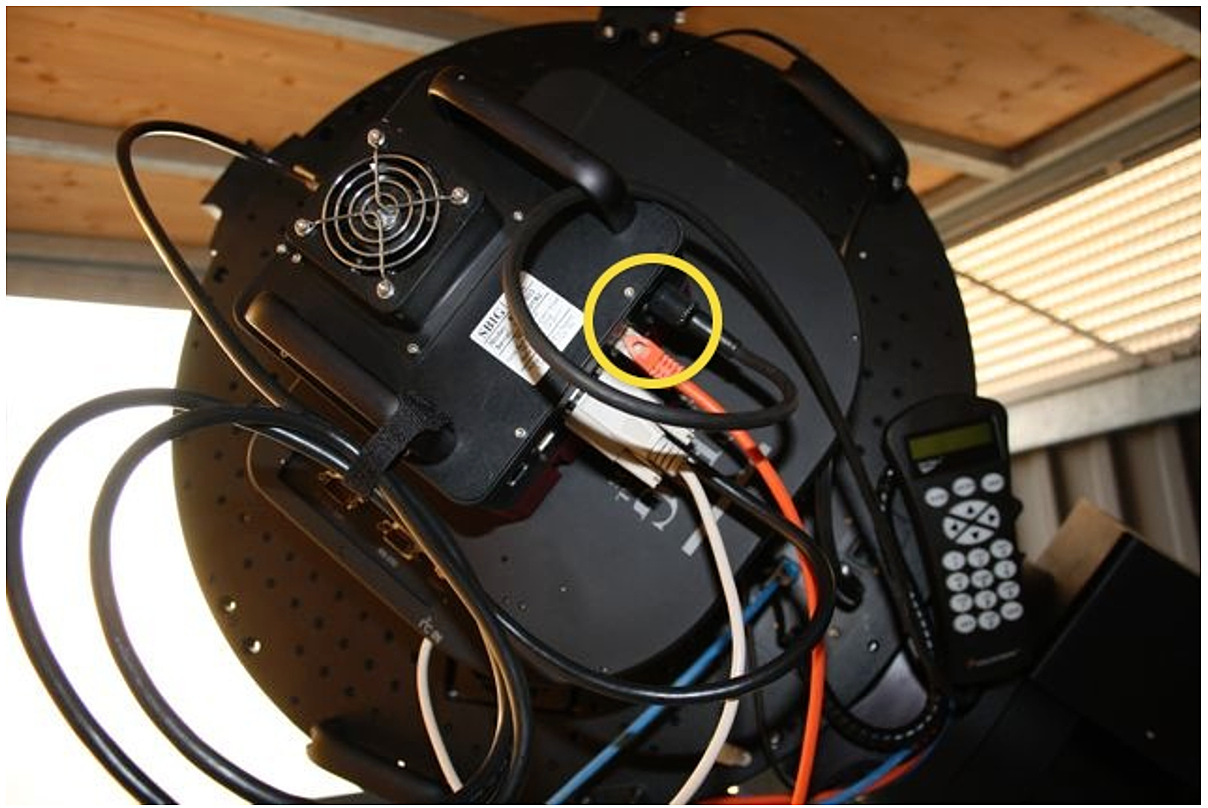
\includegraphics[width=\textwidth]{ccd-cables}
        \caption{Attaching the camera power cable and the USB cable.
            Note: In this image, the Ethernet cable is used, but the USB cable should be used instead.
        }
        \label{fig:camera-cables}
    \end{subfigure}
    \caption{Mounting the camera}
\end{figure}

To dismount the cameras, follow the steps in the reverse direction.
Make sure to attach the loose USB and power cables at the telescope with the cable strap, such that they do not get stuck when the telescope moves.

Do not remove the filter wheel from the camera unless absolutely necessary, since the filters are fragile and sensitive to dust and scratches.
The filter wheel position sensor can also easily be damaged when the filter wheel is opened incorrectly.

\chapter{Visual observation}

This chapter mostly explains how to use the hand controller.
All features of the hand controller can also be used from inside the control room, using the \texttt{Virtual Keypad} program.

\section{Hand Controller}

This section is an overview of the basic functions of the hand controller for the 10micron \textsc{gm4000} mount.
For more details, refer to the printout of the manual in the big binder in the control rool.

\subsection{General Navigation}

Press \texttt{Menu} to start, and use the up/down +/- keys (not the \texttt{E/W/N/S} keys) to navigate through the menu.
Select submenus and initialize actions with \texttt{Enter}.
Use \texttt{Esc} to return to the previous menu.
Outside the main menu, where the display shows the \textsc{ra/dec} coordinates, use the quick access buttons indicated on the keys to directly enter various object catalogs for selecting new targets and for using the automatic goto options.
The \texttt{E/W/N/S} keys can be used for manually slewing the telescope to a given position (after unparking the mount, see below).
To change the slew speed, go to the \textsc{ra/dec} screen and use the up/down keys.

Note that the telescope will stop moving automatically as soon as you hit one of the \texttt{E/W/N/S} keys or the \texttt{Stop} key.

\subsection{Parking and unparking the telescope}

For storage inside the dome, the telescope has to be in a fixed parking position, which is predefined in the hand controller.
While the mount is in the parked state, the telescope cannot move.
To park or unpark the telescope, follow these steps:

\begin{itemize}
    \item Press \texttt{Menu}.
    \item
          Use the up/down keys (not the \texttt{E/W/N/S} keys) to select \texttt{Alignment}, and press \texttt{Enter}.
    \item
          Select \texttt{Unpark/Park}, and press \texttt{Enter} twice.
\end{itemize}

Note that unparking the mount changes its state, but the telescope remains in its parked position until it receives a command to move.

\subsection{Tracking Speed}

Depending on the object you observe, you may have to change the tracking speed manually.
To change the tracking speed, press \texttt{Menu -> Drive -> Tracking speed}.
You can choose between
\begin{itemize}
    \item \emph{sidereal}, for tracking object outside the solar system (stars, galaxies, etc.)
          ,
    \item
          \emph{solar}, for tracking solar system objects (planets)
    \item
          \emph{lunar}, for tracking the moon,
    \item
          \emph{custom}, for tracking a custom orbit, and
    \item
          \emph{stop}, to stop the tracking motors.
\end{itemize}

\subsection{Slew Rate}

The slew rate is usually set at 2 degrees per second, and it should remain at this value to avoid mechanical problems with the mount, especially in winter.
However, it can be adjusted if necessary, under \texttt{Menu -> Drive -> Slew Rate}.
The slew rate can now be adjusted with the up/down keys.

Note that the slew rate affects both the manual and automatic slewing modes, so be careful not to set it too high when manually slewing the telescope.

\subsection{Manual alignment}

It is usually preferable to perform an automatic alignment with software such as \texttt{Mount Wizzard}, which can achieve pointing with sub-10-arcsecond accuracy across the entire sky.
However, sometimes it might be preferable to perform a manual alignment.
This section shows the procedure for doing this.

Note that you can safely adjust the alignment without losing the current alignment model.
You can always go back to a previous alignment model using \texttt{Menu -> Alignment -> Align Database -> Load Model}.

To perform a new alignment, press \texttt{Menu -> Alignment -> 3-Stars}, and follow the instructions on the display.

The alignment procedure for the mount requires the calibration and centering of three reference stars, which may be supplemented by a few extra stars scattered throughout the sky to refine the mount model.
Choose bright stars from the list suggested by the software, preferably widely scattered on the sky, visible, and known to you.
The telescope will then slew to the coordinates of the chosen star, and you can use the \texttt{N/S/E/W} keys to center the star on the camera or the eyepiece.
After centering the star, confirm it and proceed to the next star.

Note that for the first three reference stars, it is not possible to cancel the calibration and choose a different star if the initially selected star is not visible, such as in the case of clouds.
Once the three reference stars are calibrated, additional stars can be added to refine the mount model.
You can choose to abort the process if a star is not visible.
Generally, six stars, including the three reference stars, are enough for accurate pointing.

Do not forget to save your model under \texttt{Menu -> Alignment -> Align Database -> Save Model}, such that it can still be used after restarting the mount.

\chapter{Imaging}
This section is still under construction.

\section{Overview}
The instruments can be operated remotely from the computer in the control room via \texttt{Remote Desktop}.

\subsection{Login information}
\begin{itemize}
    \item
          Control room computer
          \begin{itemize}
              \item
                    Username: \texttt{optical}
              \item
                    Password: See printed manual
          \end{itemize}
    \item
          Telescope computer
          \begin{itemize}
              \item
                    Username: \texttt{astro-user}
              \item
                    Password: See printed manual
          \end{itemize}
\end{itemize}

\subsection{Software}
The following software on the remote computer can be used:
\begin{itemize}
    \item \textbf{\texttt{N.I.N.A.
              }} is the main control software for the telescope.
    \item
          \textbf{\texttt{PWI3}} connects to the back-panel of the telescope, which controls the fans, the focusser, the heaters, and the temperature sensors.
          It is usually not necessary to change anything here.
    \item
          \textbf{\texttt{Stellarium}} is used to select observation targets and check their properties.
          It also has a preview for the field of view of the telescope.
    \item
          \textbf{\texttt{Clock sync}} is used to synchronise the clock of the mount with the clock of the computer, which is kept accurate via the internet.
    \item
          \textbf{\texttt{Virtual keypad}} can be used to control the mount with the same interface as on the hand controller.
    \item
          \textbf{\texttt{Mount Wizzard}} is a \texttt{Python} script (currently residing in the Downloads folder) for automatically aligning the telescope with arcsecond accuracy.
    \item
          \textbf{\texttt{ASTAP}} is a program for calibrating and stacking images.
          While it is quite convenient, note that it cannot perform background subtraction on individual frames, which makes it somewhat unsuitable for scientific data analysis.
          You can use it for astrometric calibration though.
\end{itemize}
The following sections explain in more detail how the software can be used to perform observations.

\section{N.I.N.A.: Instrument operation}

\subsection{Start-up}\label{sec:NINA:start-up}

First, all relevant instruments have to be connected. This includes the camera, the filter view and the mount. The order does not matter. Connect the individual parts by navigating to them in the equipment tab (make sure you have selected 'Equipment' all the way on the left) and then clicking on the on/off button at the top. Each time a successful connection has been made, you should see a confirmation message on the bottom right. Additional windows might open, just ignore them for now, but do not close them. For the camera, the cooling has to be engaged and the mount must be unparked using the respective buttons. Refer to the figures below.
\begin{figure}
    \centering
    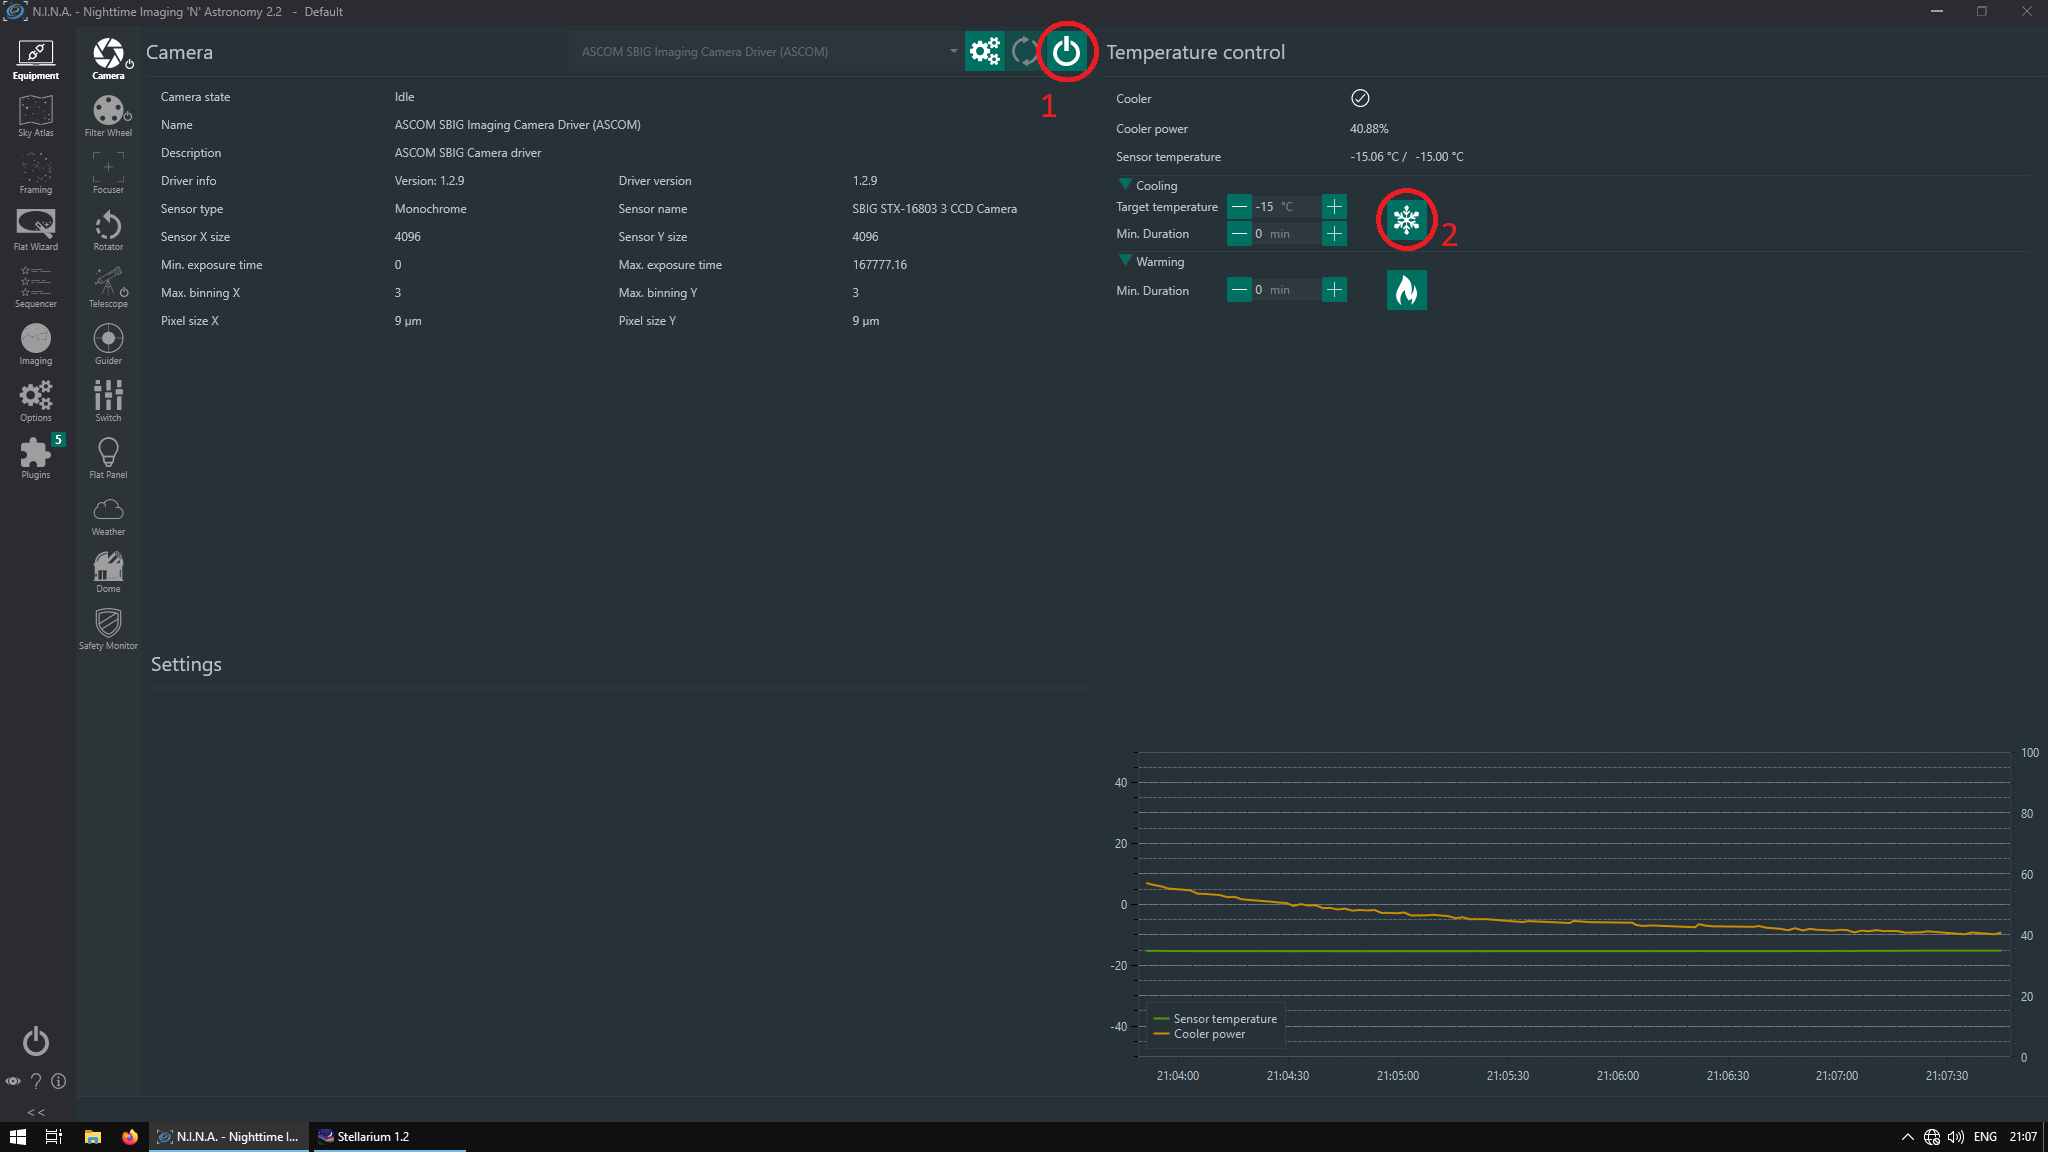
\includegraphics[width=0.85\textwidth]{figures/NINA/CameraDP.png}
    \caption{Connecting the camera. Select 'Camera' on the equipment tab, then connect the camera using the on/off button. Afterwards, check that the cooling is set to $-15\,\si{\degreeCelsius}$, then click on the snowflake to engage cooling. Make sure the temperature drops as expected. If the cooling gets 'stuck', simply repress the snowflake button. The same goes for the flame button when shutting down the equipment.
    }
    \label{fig:NINA:Camera Connection}
\end{figure}

\begin{figure}
    \centering
    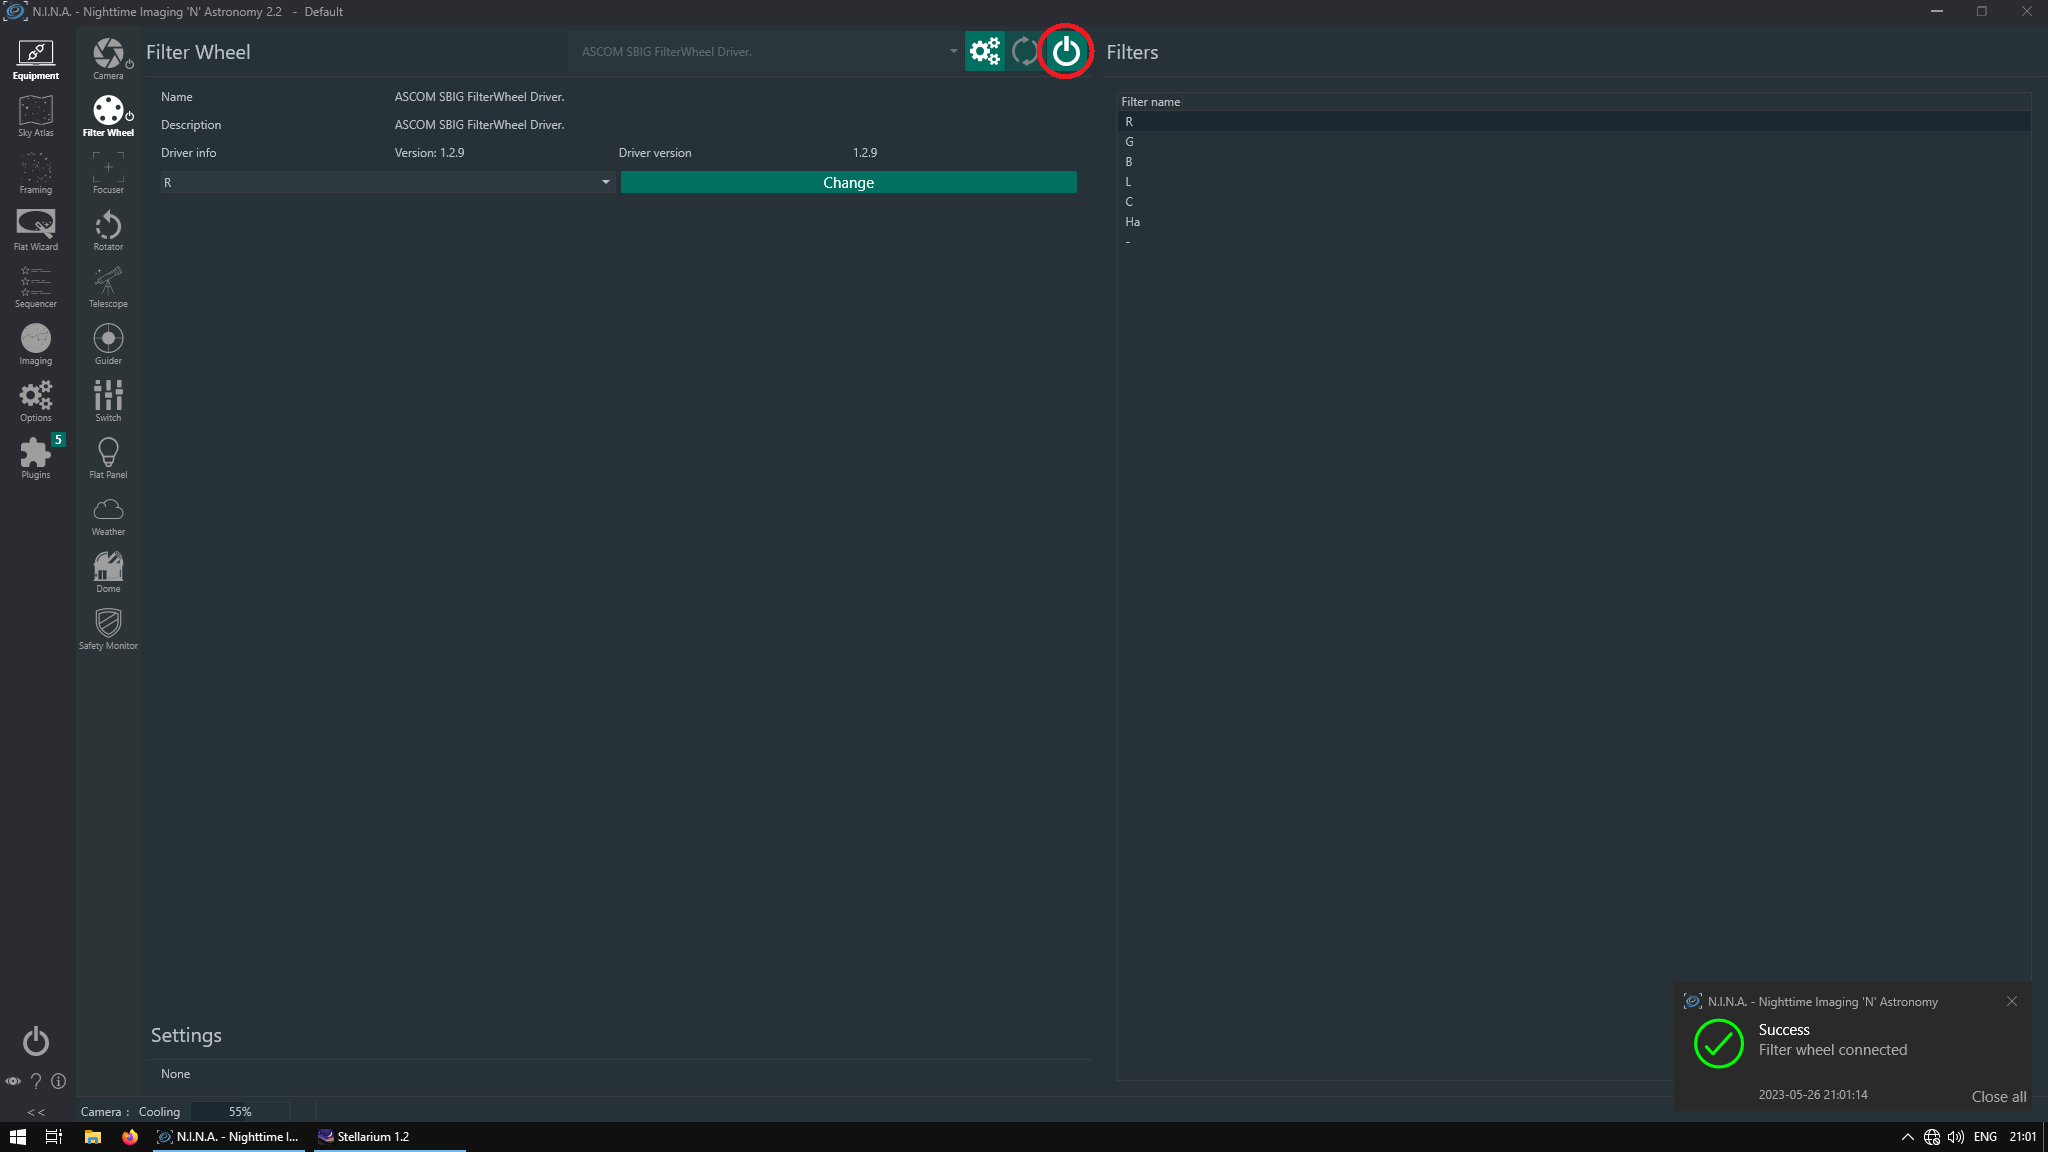
\includegraphics[width=0.85\textwidth]{figures/NINA/FilterDP.png}
    \caption{Connecting the filter wheel. Select 'Filter Wheel' on the equipment tab, then connect the the wheel using the on/off button.
    }
    \label{fig:NINA:Filter Connection}
\end{figure}

\begin{figure}
    \centering
    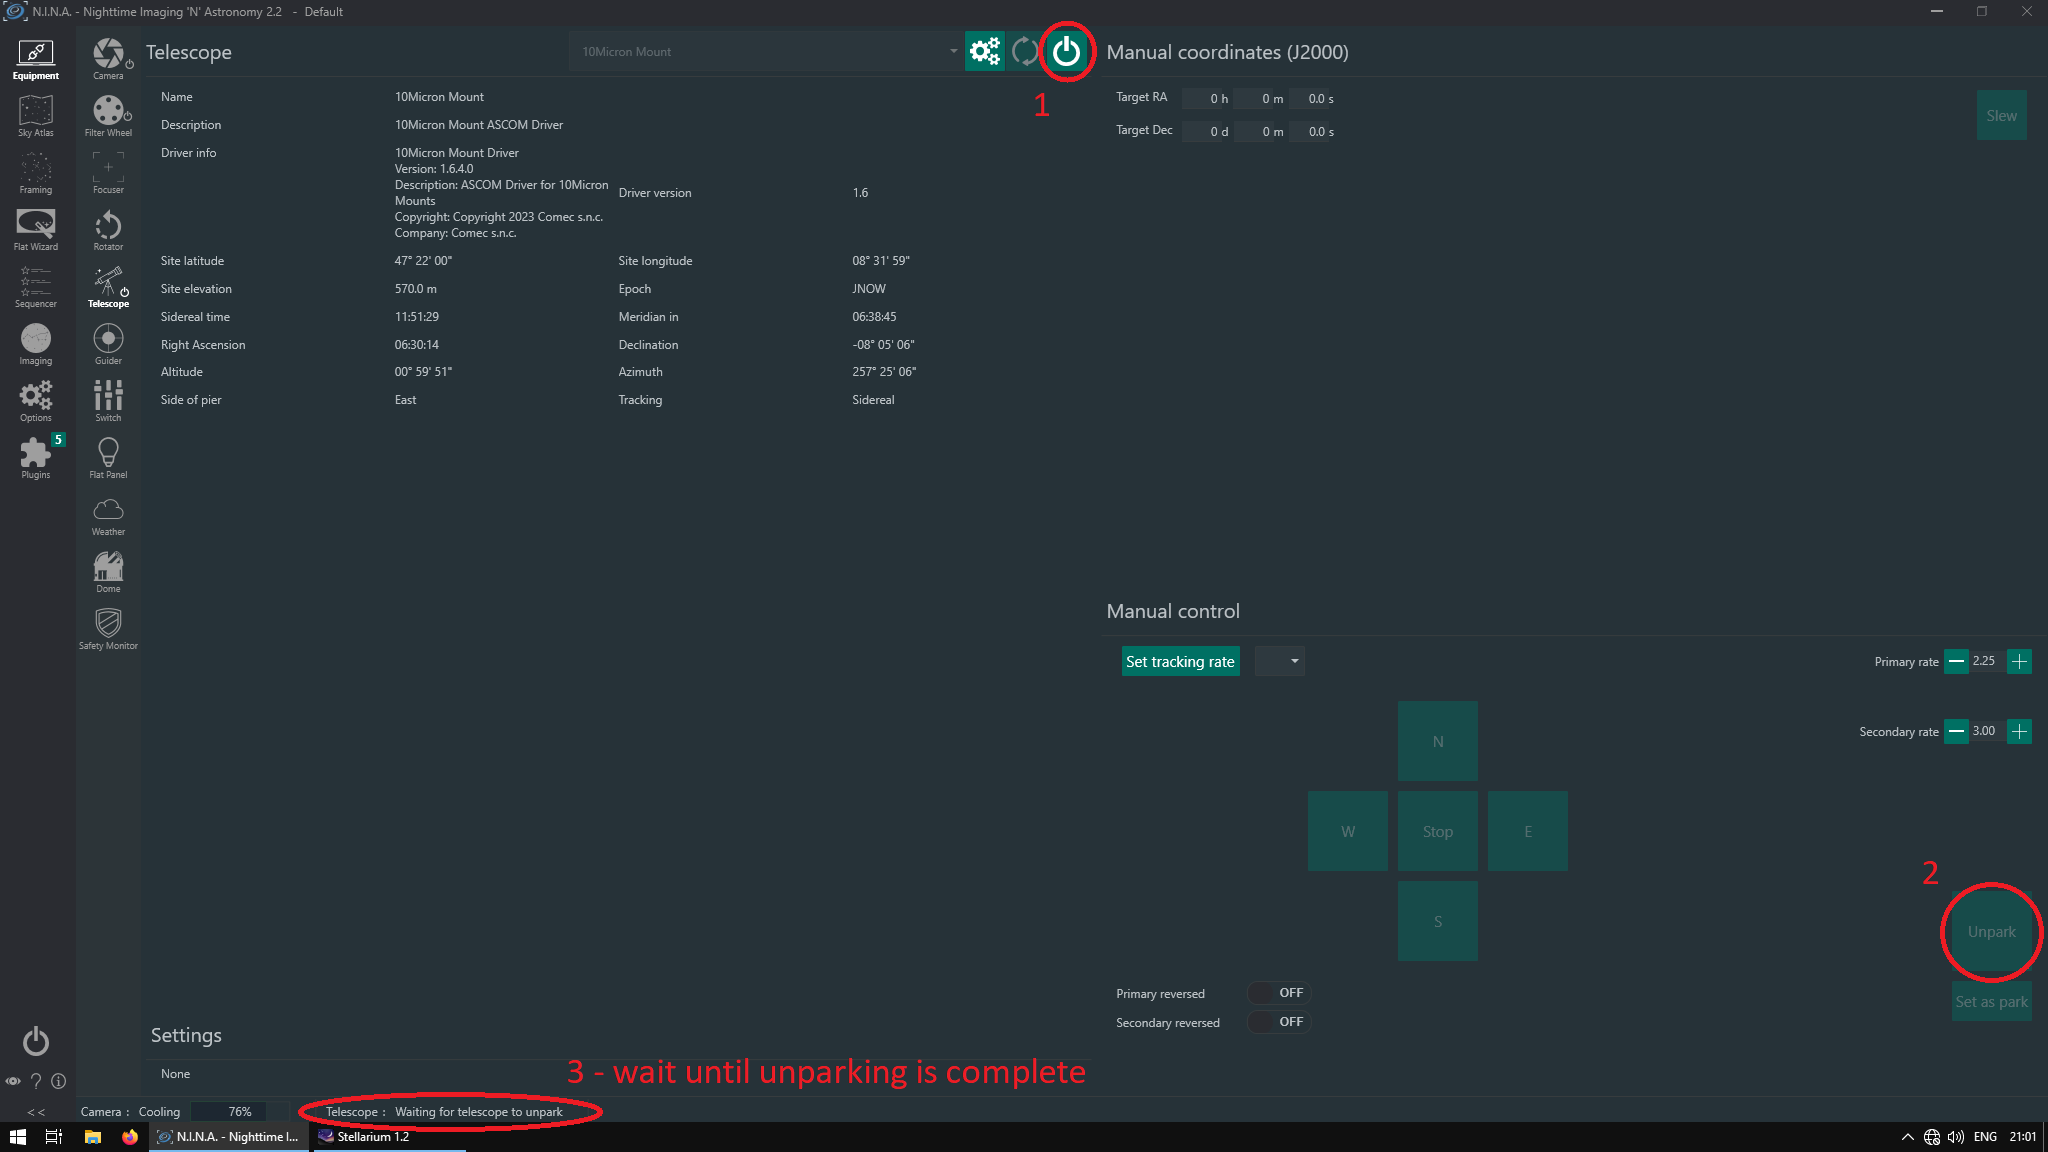
\includegraphics[width=0.85\textwidth]{figures/NINA/TelescopeDP.png}
    \caption{Connecting the telescope. Select 'Telescope' on the equipment tab, then connect the telescope using the on/off button. After the connection has been made, the mount must be unparked from home position. Press the "Unpark" button and wait for the telescope to complete the request (trackable by the message at the bottom).
    }  \label{fig:NINA:Telescope Connection}
\end{figure}
% Connect instruments, cool the camera (might have to re-press if it gets stuck) Unpark the mount. TODO DONE

\subsection{Slewing}\label{sec:NINA:slewing}

In order to slew to a target, you can first select it in Stellarium. Stellarium also allows for the configuration of the telescope specs, which gives a good preview of the expected field of view. You can set this up by entering the telescope details into the settings of Stellarium (refer to the figures \ref{fig:NINA:choose_sensor_final} and \ref{fig:NINA:gear_selection_final}). If the right telescope and CCD sensor do not exist, you can manually enter them by clicking on 4. in \ref{fig:NINA:choose_sensor_final} and adding the two new devices with the data given by the left two images of \ref{fig:NINA:gear_selection_final}. Clicking on 3. (in \ref{fig:NINA:choose_sensor_final}) allows you to select the telescope (1.) and the sensor (2.).

\begin{figure}
    \centering
    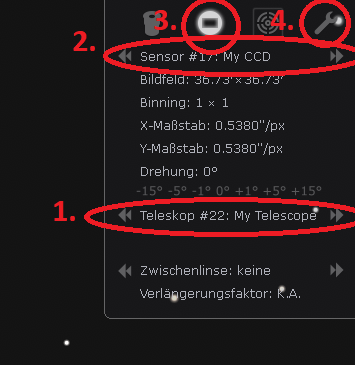
\includegraphics[width=0.45\textwidth]{figures/NINA/choose_sensor_final.PNG}
    \caption{Select a telescope and a sensor (CCD camera) option in Stellarium.}
    \label{fig:NINA:choose_sensor_final}
\end{figure}

\begin{figure}
    \centering
    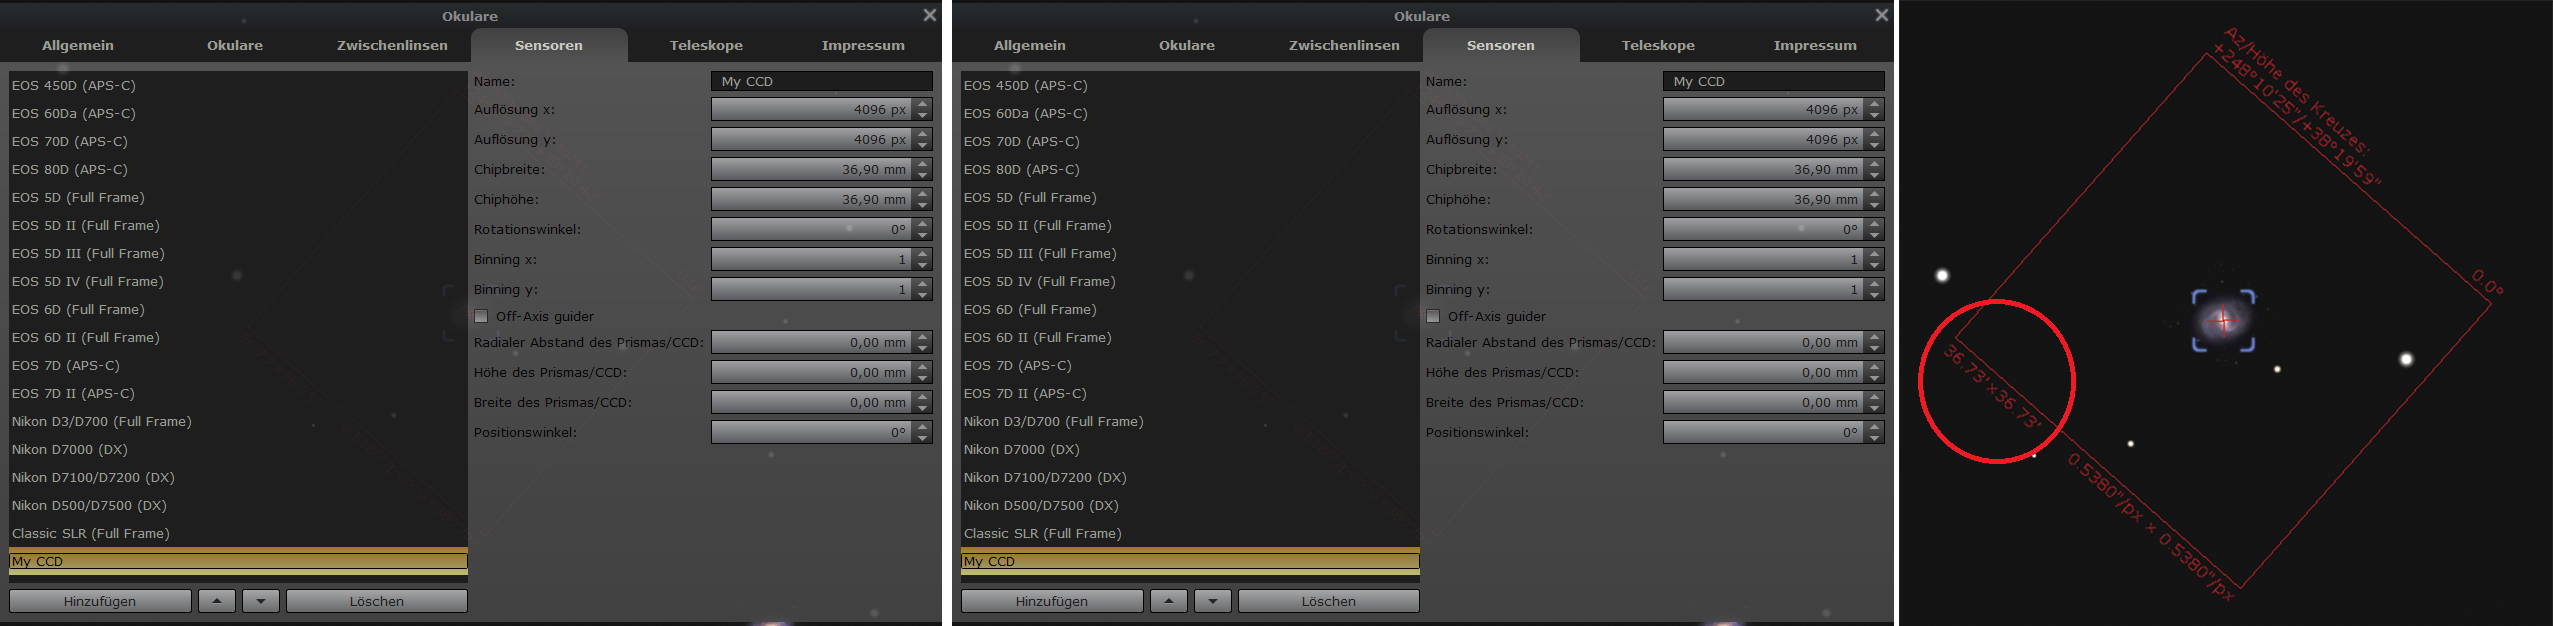
\includegraphics[width=\textwidth]{figures/NINA/gear_selection_final.png}
    \caption{Configurations for telescope and CCD setup (left two). The right image shows the view for the in 1. and 2. of \ref{fig:NINA:choose_sensor_final} selected setup.}
    \label{fig:NINA:gear_selection_final}
\end{figure}

When you have made your target selection in Stellarium, you can directly import the coordinates and object information into N.I.N.A. In the 'Framing' tab on the left, click the import button to load the information and then press select 'Slew' from the 'Slew and center' drop-down menu to slew the telescope to the object. Make sure to wait until the slewing is complete to take images.

\begin{figure}
    \centering
    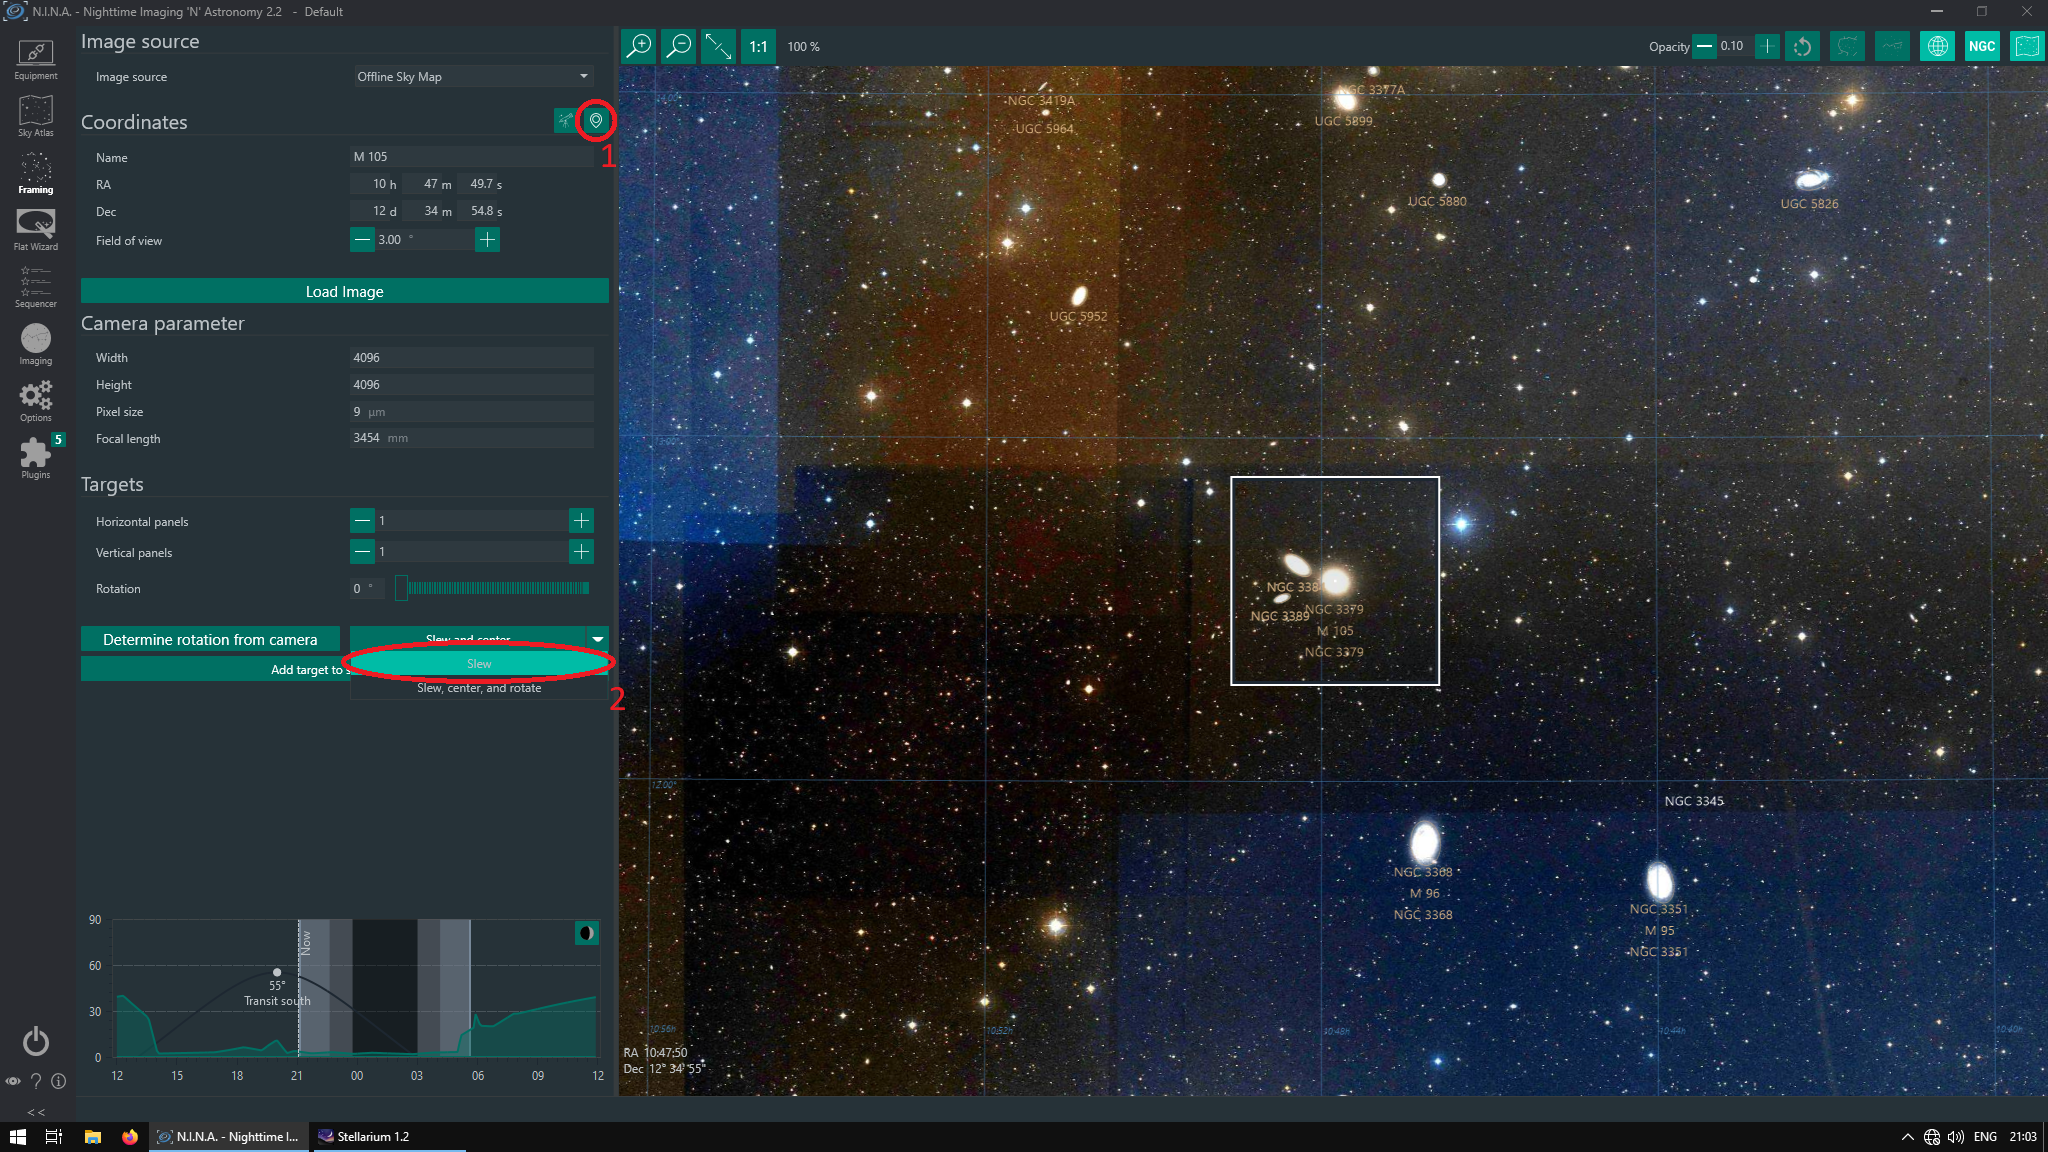
\includegraphics[width=0.85\textwidth]{figures/NINA/ImportAndSlew.png}
    \caption{Importing object information from Stellarium and slewing. In the 'Framing' tab on the left, import the currently selected object from Stellarium. Afterwards, select 'Slew' from the 'Center and Slew' drop-down menu to slew the telescope to the target object.}
    \label{fig:NINA:ImportAndSlew}
\end{figure}

Keep in mind that slewing does not work (is greyed out) while the camera is taking exposures. Stop the camera first.
Similarly, you cannot take images while the telescope is still slewing.

%\subsection{Imaging}

\subsection{Single image exposure}\label{sec:NINA:single_image_exposure}
To take a single image, you first need to navigate to the 'Imaging' tab on the left. 
There are four parameters you should know for your exposures:
\begin{itemize}
    \item \texttt{Exposure time}: the duration the CCD should be exposed to the incoming light.
    \item \texttt{Filter}: The bandwidth filter which to use, i. e. which part of the spectrum you want to capture.
    \item \texttt{Binning}: How many pixels should be averaged to compress the image (e. g. 2x2 averages each 2x2 square to one output pixel).
    \item \texttt{Loop}: Whether you want to take a single exposure or loop several after one another.
    \item \texttt{Save}: Whether you would like to save the resulting images (as FITS files).
    \item \texttt{Enable sub-sampling}: Whether to take individual exposures of parts of the detector. This is usually not needed for the experiments and is disabled by default.
\end{itemize}
If you do not know the ideal exposure time based on signal-gain ratio, there is a built-in tool: In the navigation bar on the bottom, click on 'Optimal Exposure Calculator'. Then, set the 'Exposure time' field appropriately. You might need to test a few values here based on the object, since too short of an exposure will not yield enough signal and too long could over-saturate the detector, falsifying the results. Do not change the other values in the calculator. Start the computation by clicking on the large shutter button.
\begin{figure}
    \centering
    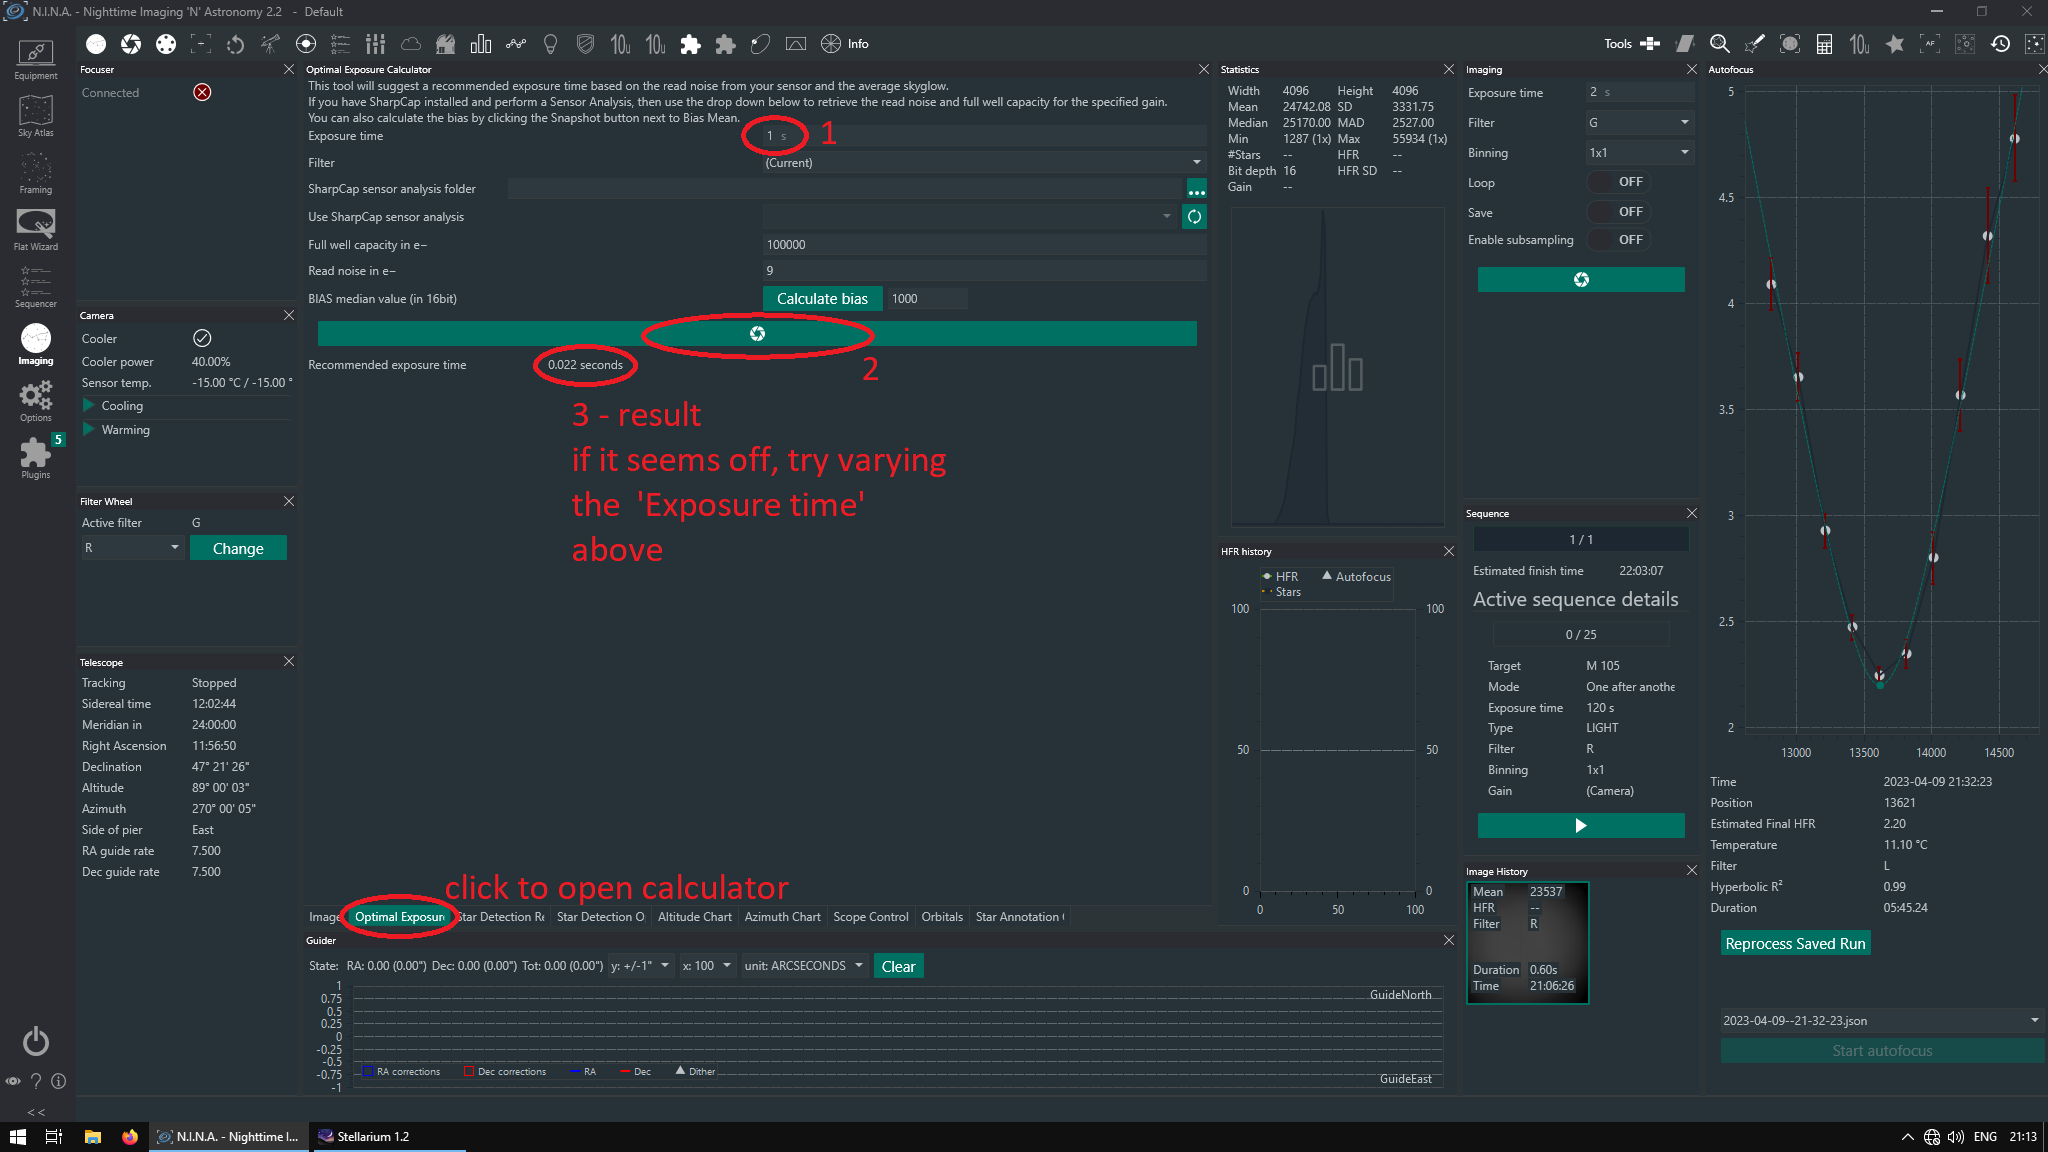
\includegraphics[width=0.85\textwidth]{figures/NINA/ExposureCalculator.png}
    \caption{How to use the exposure time calculator. First, open it by using the lower navigation bar. Enter a trial exposure time and click on the shutter to compute the ideal exposure time. If the result seems off, the detector could be over- or under-saturated. Try varying the trial exposure.}
    \label{fig:NINA:ExposureCalculator}
\end{figure}

To start an exposure, use the 'Imaging' panel with the shutter button on the top-right of the screen. After setting up the aforementioned values in their respective fields, click on the small shutter button to start the exposure. When an image is ready, you can view it by clicking on the 'Image' button on the lower navigation bar. If you enable the 'Save' option in your imaging setup, all images will be stored as FITS files inside the 'Data' folder on the desktop, categorized by date and then by filter.

\begin{figure}
    \centering
    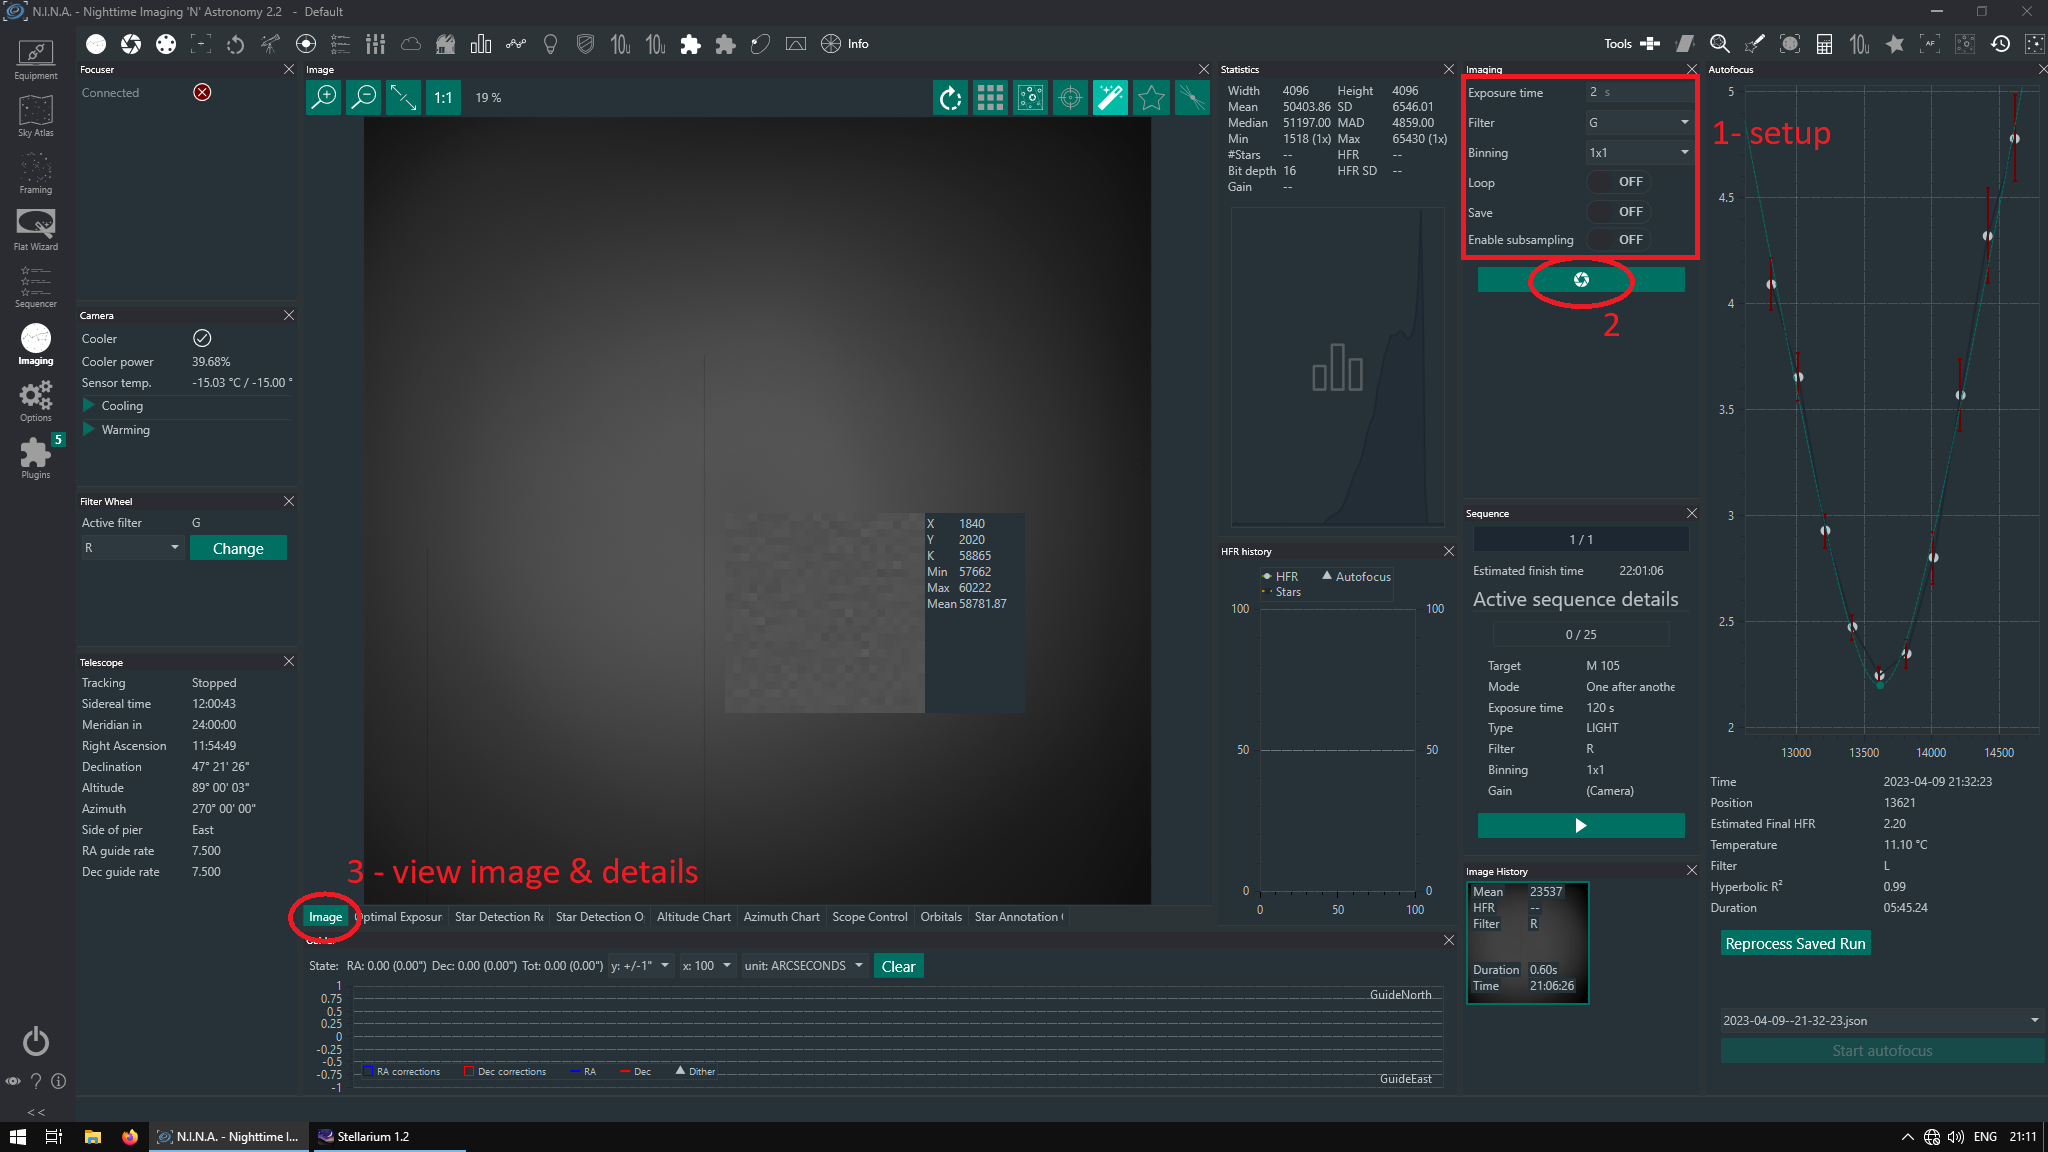
\includegraphics[width=0.85\textwidth]{figures/NINA/SingleExposure.png}
    \caption{Taking a simple exposure. First, setup your exposure by modifying the data fields in the 'Imaging' panel. Start the exposure by clicking the shutter button. When an image is ready, you can view it by navigating to 'Image' on the lower navigation bar. This also allows you to see details like the individual pixel counts.}
    \label{fig:NINA:SingleExposure}
\end{figure}


\subsection{Sequencer}

Setting up a sequence allows you to take multiple images with possibly different filters or exposure times automatically, without having to take every single frame individually as in \ref{sec:NINA:single_image_exposure}. 

The simplest way is to set up a sequence that consists of only one object using one filter and exposure time. If you want to use multiple filters or exposure times, you can just repeat the following instructions. This adds multiple different sequences grouped by objects (see ``\texttt{M101}'' in figure \ref{fig:NINA:configure_sequence_edited}), which are run through one after the other once everything is started.

The first step is to import an object into \texttt{N.I.N.A.} and to slew to it as described in \ref{sec:NINA:slewing}. Alternatively, you can also select an object by name if it is correctly entered into 1. of \ref{fig:NINA:add_to_sequence_edited}. Now, instead of switching to the \texttt{Imaging} tab, click on the little arrow 2. in \ref{fig:NINA:add_to_sequence_edited} and select 3., the \texttt{Legacy Sequencer}. This adds your object to a new and not yet configured sequence and opens a new tab. If the tab does not open, click on the \texttt{Sequencer} tab in the left vertical bar.

\begin{figure}
    \centering
    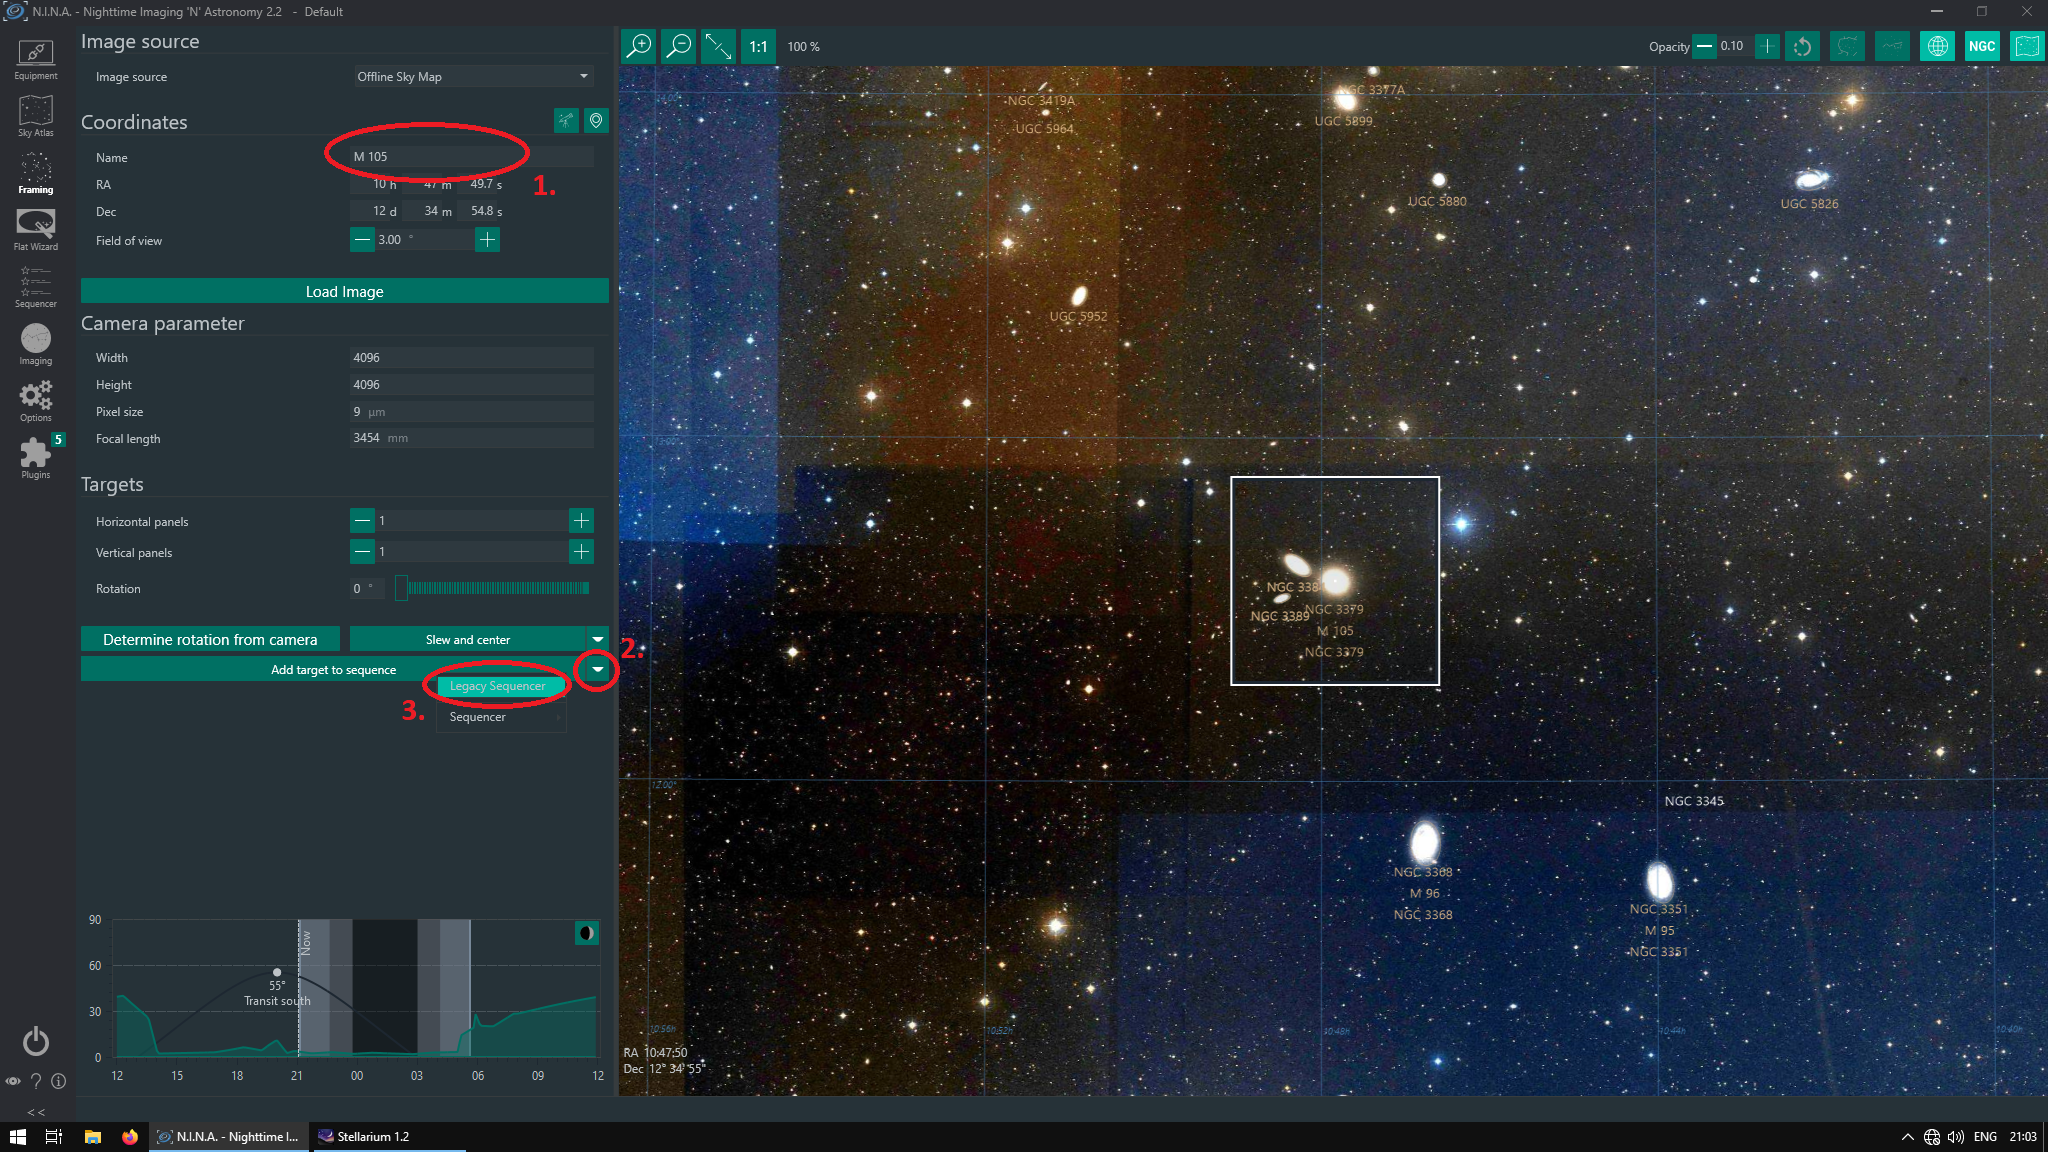
\includegraphics[width=0.85\textwidth]{figures/NINA/add_to_sequence_edited.png}
    \caption{Steps to add an object that was selected e.g. using \texttt{Stellarium} to a sequence using the \texttt{Legacy Sequencer}.}
    \label{fig:NINA:add_to_sequence_edited}
\end{figure}

The next step is to configure the sequence with the obeject that was just added. There are a few basic steps and possible options that are outlined in the following list. Each list item corresponds to the number as written in figure \ref{fig:NINA:configure_sequence_edited}.

\begin{figure}
    \centering
    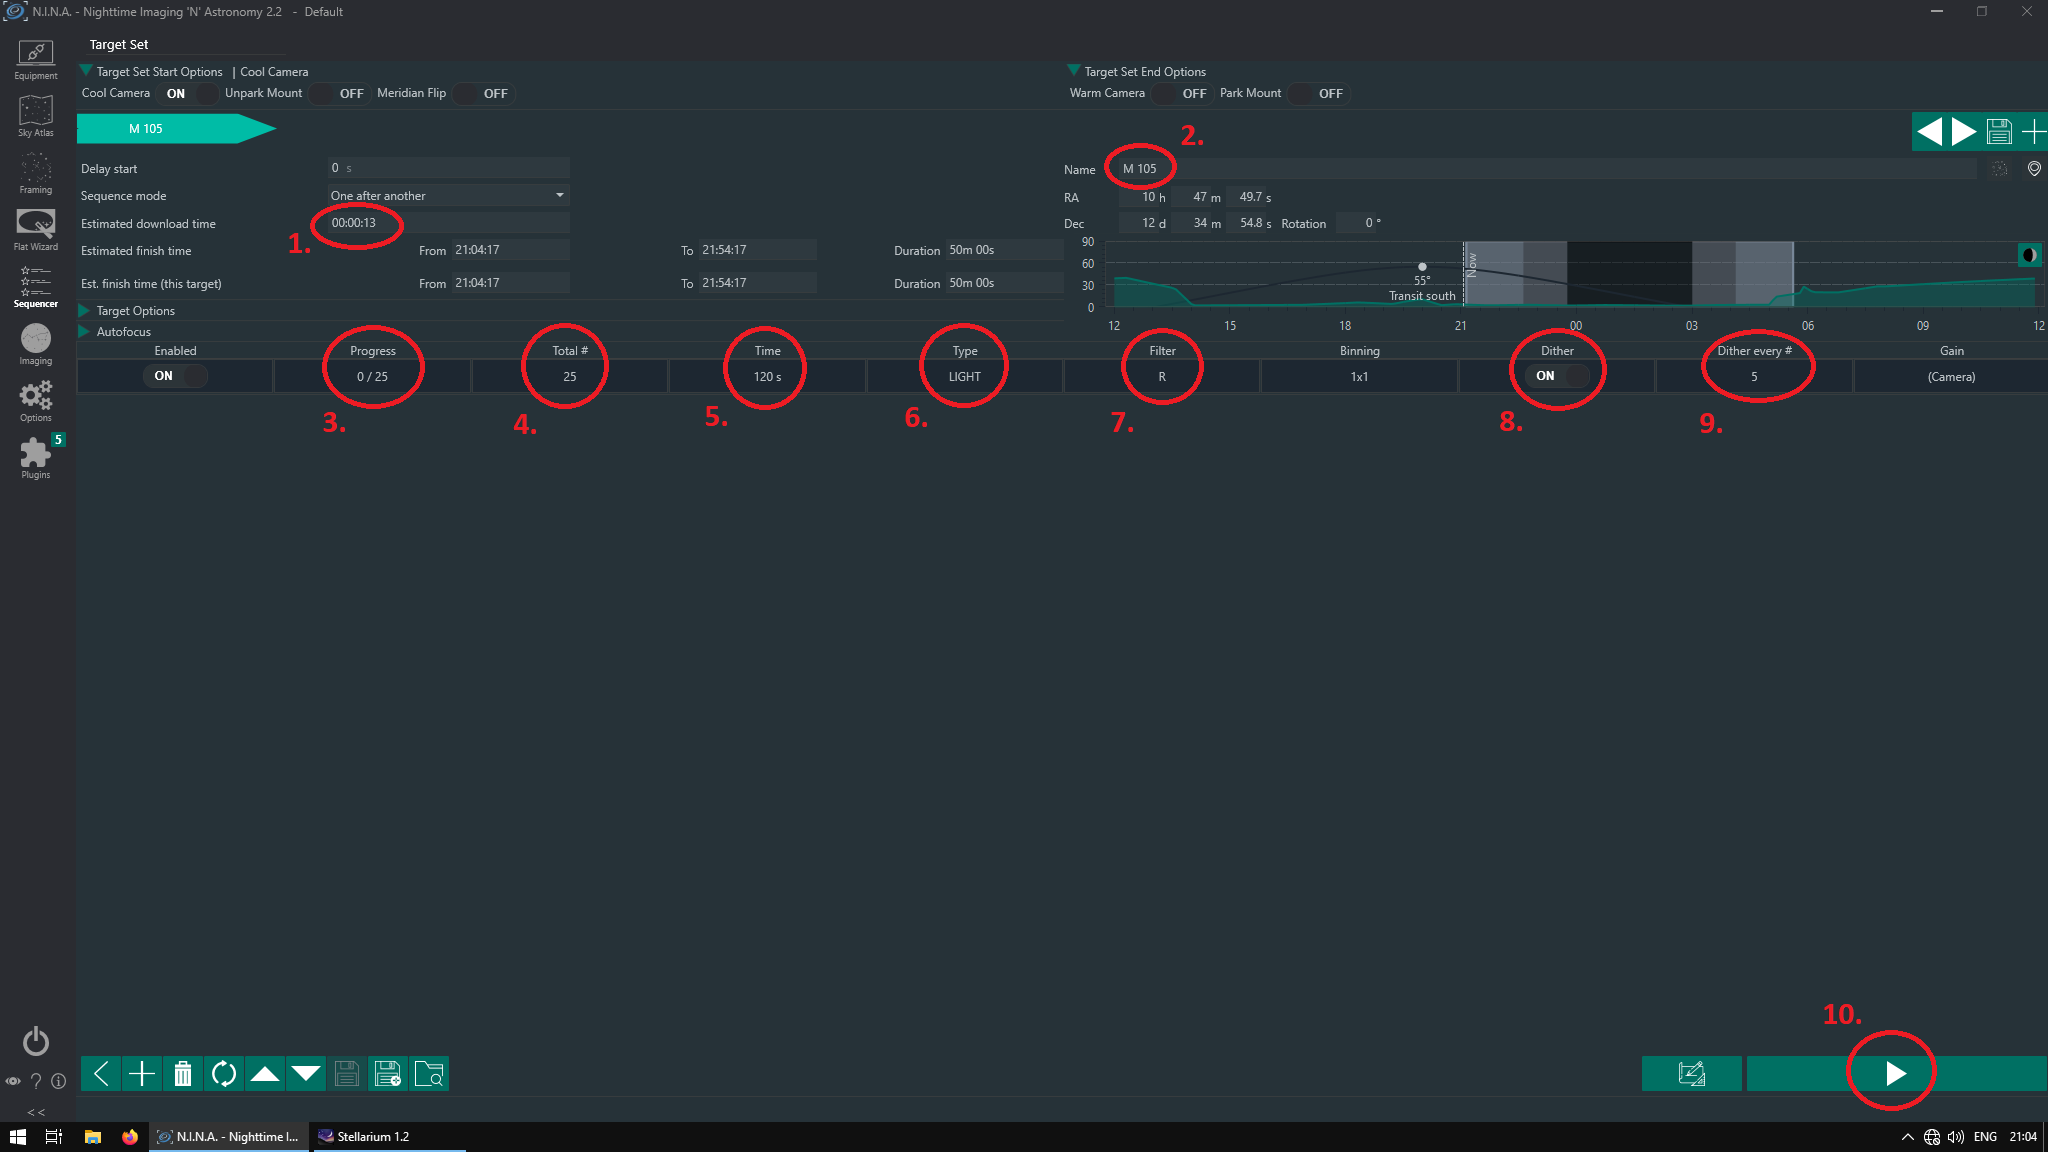
\includegraphics[width=0.85\textwidth]{figures/NINA/configure_sequence_edited.png}
    \caption{Steps to configure a sequence if the object was already added as a \texttt{Legacy Sequence}.}
    \label{fig:NINA:configure_sequence_edited}
\end{figure}

\begin{enumerate}
    \item This field allows you to give a time the CCD needs to read out the image. The usual value for the current camera (June 2023) is $13\,\si{\second}$. This allows for a more accurate ETA estimation.
    \item This is the name you want to give this object. The standard value is its catalogue name. This mainly determines the name of the folder that will be created in which all exposures will be saved. The saves are sorted by type, then filter and then contain the exposure time and numeration in the title.
    \item This field gives you the number of frame already saved once the sequence is started. This field is not important during setup.
    \item Here you select the number of frames to be taken using the following specifications.
    \item Here you simply select the exposure time (that you either calculated using SNR or using the optimal exposure calculator that is located in the \texttt{Imaging} tab).
    \item Here you select your frame type. \texttt{LIGHT} are normal exposures of your object. \texttt{FLAT}, \texttt{DARK}, \texttt{BIAS} and \texttt{DARKFLAT} are your calibration frames (if you take them manually without using the \texttt{FLAT Wizard}). \texttt{SNAPSHOT} are test frames that you might want to save but not use in you final result.
    \item Here you select your filter (R - red, G - green, B - blue, L - luminance, Ha - $H_\alpha$ band filter). If your filterwheel is currently at a different position, the sequence will automatically switch it.
    \item Activate dither to minimally change the position of the telescope every view frames. This allows e.g. to later correct for broken pixel columns using for example sigma clipping.
    \item Here you can enter after how many frames the telescope is supposed to slightly change its position (``dither''). 
\end{enumerate}
If everything was set to your will, you can click on 10. in \ref{fig:NINA:configure_sequence_edited} to start the sequence.



\subsection{Focus}

In order to access focus settings, click on the \texttt{Imaging} section located on the left vertical selection bar (see 1. in figure \ref{fig:NINA:focusing_tab}). If the square containing the focus parabola is not visible, click on symbol 2. in \ref{fig:NINA:focusing_tab} to open it. 

\begin{figure}
    \centering
    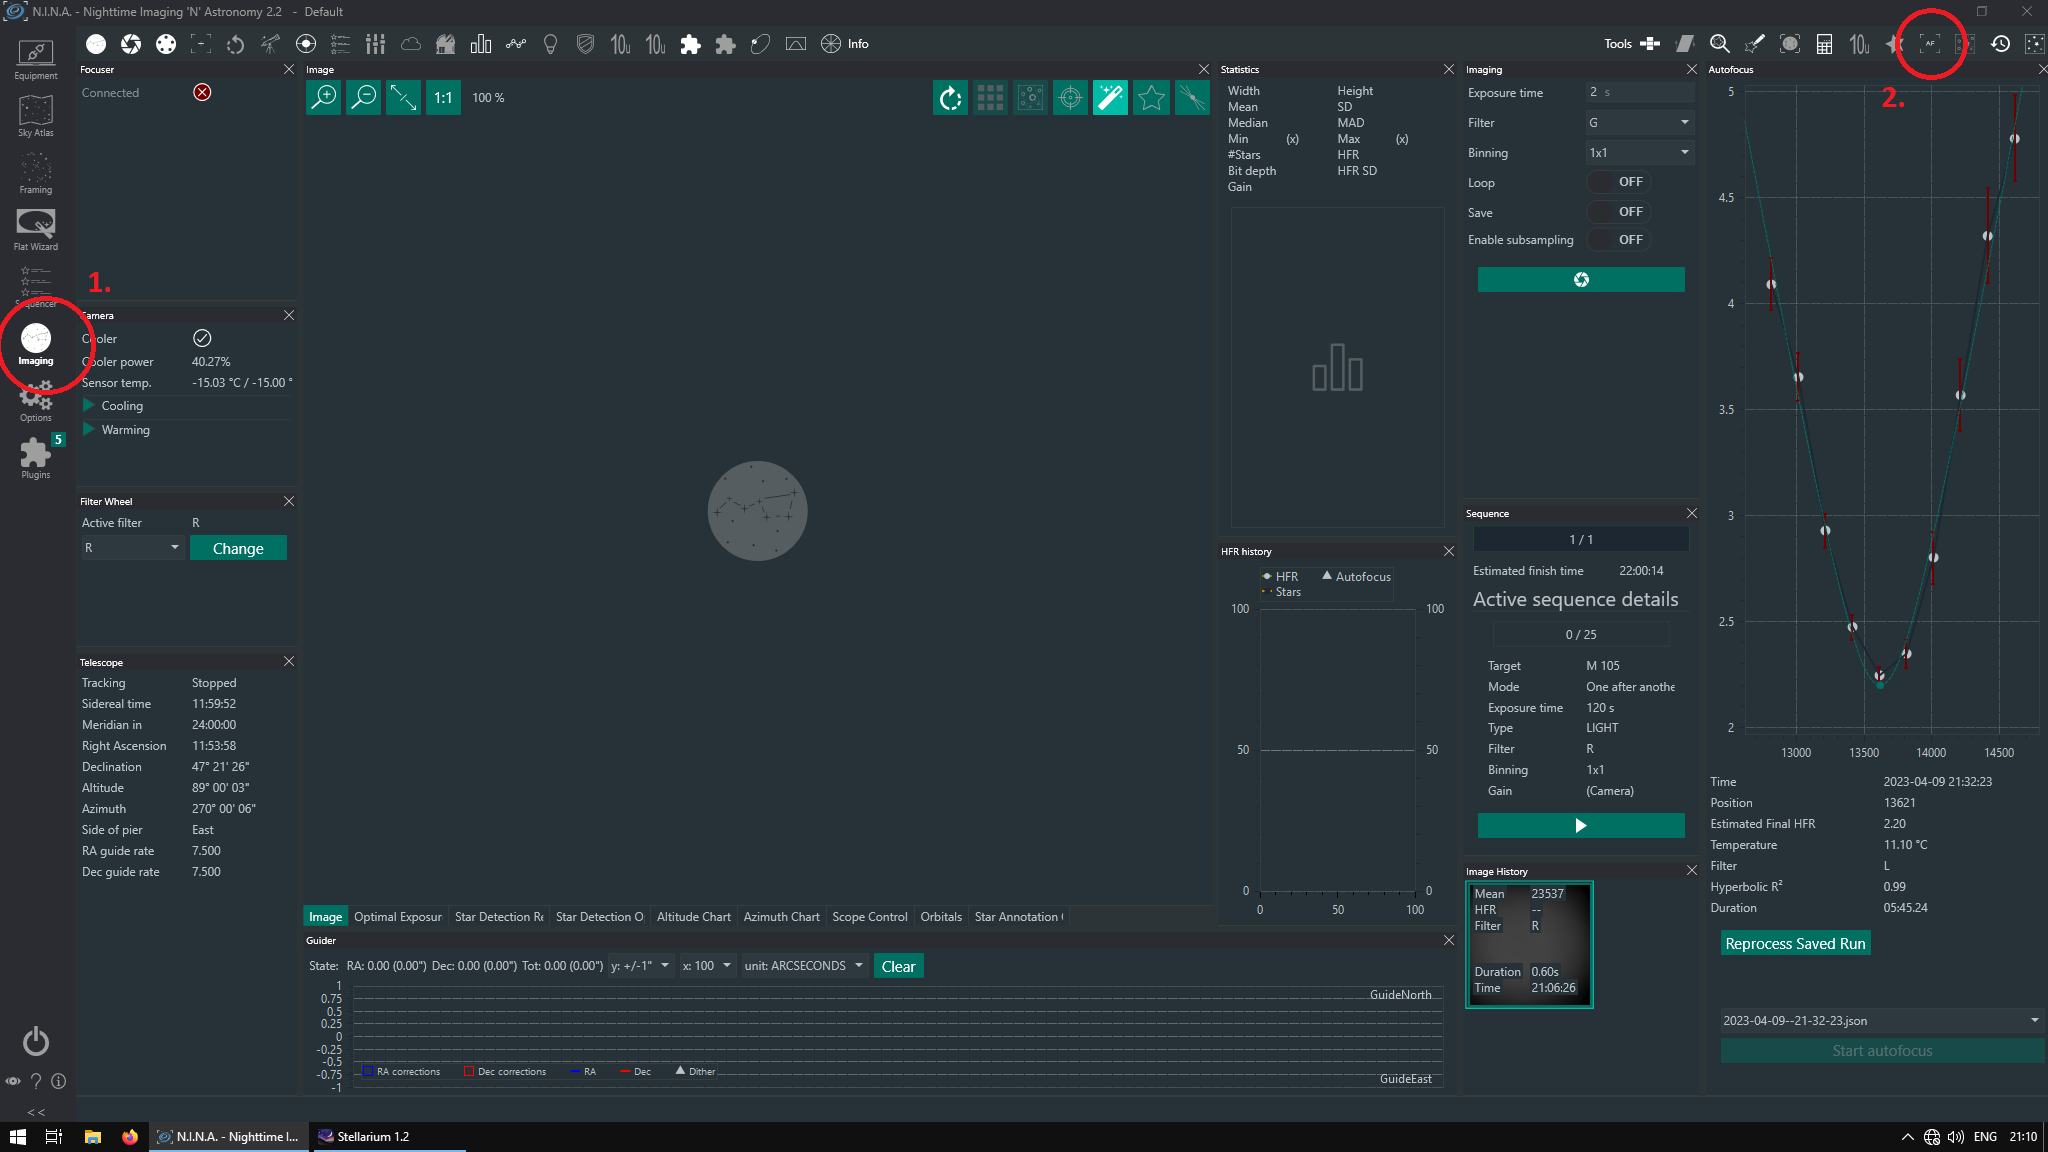
\includegraphics[width=0.85\textwidth]{figures/NINA/focusing_tab.png}
    \caption{Focus menu (top right box) in N.I.N.A.'s imaging section.}
    \label{fig:NINA:focusing_tab}
\end{figure} % TODO add where to find the focus tab, and what to do if it is hidden.

% TODO how to manually go to a fixed focus position
The telescopes focus is controlled via a focuser that can also be connected in the \texttt{Equipment} tab, there you can insert a manual focus position, which corresponds to the $x$-axis in the focus tab in \ref{fig:NINA:focusing_tab}. This is (as well as the step before) is usually not necessary, if the TA did not specifically request it or one of the conditions in the following apply. 

The focuser position is displayed in micrometers.
Usually, focus is between 10000 and 15000 micrometers.

There are several scenarios where changing the focus is necessary:
\begin{itemize}
    \item The camera has just been removed and reinstalled at the telescope.
    \item
          The focusser has been recalibrated using the PWI3 software.
    \item
          Autofocus has not been performed for a while (a few weeks), and the position has slowly drifted away
    \item
          The filter of the filter wheel is changed. (This is automatically compensated by N.I.N.A. by moving the focusser by a known offsets each time the filter is changed.)
\end{itemize}

It is very good practice to perform an autofocus before beginning an observing night.
The focus will usually remain good for the entire night, and probably even a few weeks.
Images taken with bad focus are usually not usable, with a few exceptions if you know what you are doing.

\subsubsection*{Autofocus procedure}
To perform an autofocus:

\begin{enumerate}
    \item Slew to a position where there are many separate stars visible (e.g. towards the center of the Milky Way, or check in Stellarium).
          \footnote{In doubt, it is better to have too many bright stars, rather than few
              dim stars.
              The algorithm is usually quite resilient and can deal with some disturbances, such as saturated stars, galaxies, nebulae etc. Just make sure that the star is not so bright that it covers a large fraction of the sensor.
          }
    \item
          Take a test exposure in the L filter with an exposure time of 3 seconds.
    \item
          Check that there are many separate stars visible in the picture.
          Stars that are very faint, saturated, or not well separated cannot be used for autofocussing.
          \footnote{To check the brightness of a star, hover over the image, and hold right click.
              This will open a small window that shows some statistics in a small area around the cursor.
          }
          \begin{itemize}
              \item
                    If the image is already strongly out of focus, (e.g. you see donut rings instead of stars, or no stars at all), try to manually find a position between 10000 and 15000 where stars are nicely visible.
          \end{itemize}
    \item
          (Optional) Check the autofocus settings in N.I.N.A. under \texttt{Settings -> Autofocus}.
          Adjust the parameters only if something does not work.
    \item
          In the Imaging tab, click \texttt{Autofocus}.
          The filter will be automatically switched to L, to get bright stars.
    \item
          Wait for focus to finish.
          Once done and successful, the focusser will automatically move to the best focus position.
\end{enumerate}

During autofocus, a focus hyperbola will be estimated.
The vertical axis shows the half-flux radius (\textsc{hfr}) in arcseconds, and the horizontal axis the focusser position in micrometers.
The autofocus procedure will move the focusser to a range of focus positions, take an image at each position, and determine the average \textsc{hfr}.
The lower the \textsc{hfr}, the smaller the stars, and the better the focus.
For a successful autofocus, the measurement of \textsc{hfr} as a function of focusser position is a hyperbola.

An excellent focus will have a \textsc{hfr} of about 2, an acceptable one about 3, and a terrible one about 5. A nice example of such an parabola can be seen on the right side of figure \ref{fig:NINA:focusing_tab}.  % DONE Add an image of a nice focus hyperbola here.


\subsubsection*{Default settings} % Something else? I think that might be enough...

Here are some useful default settings when conducting the autofocus procedure:

\begin{itemize}
    \item The correct focus is usually around 12500.
          It can be from 10000 to 15000.
    \item
          To get a good range of focus positions, aim for going
          from a decent starting focus position up to about +- 1500 away from the starting position.
          This should give an HFR at about 5 to 10 at the bad ends, and a good focus in the middle.
          \begin{itemize}
              \item
                    A good setting is: set step size of 300, 5 steps either way, and start at
                    around 12500.
                    A good exposure time is a few seconds, depending on filter and field.
                    The step size can be reduced if you think you are already close to good focus
          \end{itemize}
\end{itemize}


\subsubsection*{Troubleshooting}
If the procedure does not work, first look at the focus curve that has been generated.
Your goal is to get a nice hyperbola that fits the data points well, with no outliers, and an \textsc{hfr} range from about 2 at the center to about 5 or so at the edges.
You want an $R^2$ of the fit from $0.98$ to $1.00$.
Everything else means something probably went wrong.
Still, an $R^2$ of better than $0.9$ will probably still give you a decent focus, but it is a bit uncertain.

Note that if you change any of the focus settings, you should change them back to their original setting after you finished focussing.

Here is a list of possible issues and how to fix them:

\paragraph*{There are greyed out points at an \textsc{hfr} of 0 in the focus curve.
}
If a data point is greyed out and at 0 \textsc{hfr}, this means that the star detection algorithm could not find any stars, and the image will be ignored in the autofocus procedure.
If there are still at least 5 good data points that form a hyperbola, the focus will be fine.
Otherwise, there can be two causes if too many points are greyed out:

First, all of the stars in the image may be too dim, saturated, or otherwise not suitable for focussing.
Check the brightness and quantity of the stars in the images that have failed, and maybe slew to a different field for focussing.
In rare cases, you may want to tune the star detection options.
(Make sure to reset them later!)

Second, especially if the greyed out points are towards the outer edges of the focus curve, it may be that the stars are so far out of focus that they turn into donut-shaped objects.
In this case, the star detection thinks it's not a star and ignore it.
This means that the autofocus procedure has gone too far away from a good focus.
To solve this, go to \texttt{Settings -> Autofocus}, and reduce the focus step size or the number of steps.

\paragraph*{There are points that look very wrong on the focus curve.}
This usually means that the stars could not be detected reliably, or their diameter could not be estimated reliably.
Go to a different field, or maybe increase the exposure time a little in \texttt{Settings -> Autofocus}.

\paragraph*{The focus process times out.}
Unfortunately, N.I.N.A.
is a bit impatient, and will abort the focus procedure if it takes longer than 10 minutes or so.
To solve this, make sure that a bright filter (such as L) is used for focussing,\footnote{N.I.N.A.
    knows the offsets required for all the filters, so it is sufficient to focus only using the L filter.
    If for some reason you manually have to focus with the Ha filter, try fewer steps to avoid a time out.
} the exposure time is not too long, and you are not performing to many focus steps.
You can change all of this in \texttt{Settings -> Autofocus}.

\paragraph*{The focusser does not move.}
The focusser probably thinks it has hit a mechanical limit.
This is usually just a calibration error.
Recalibrate the focusser by opening the \texttt{PWI3} software, going to \text{Focus -> Find Home}.
Note that the correct focus position may change significantly after performing the calibration.

\subsection{Autoguiding}

\begin{figure}
    \centering
    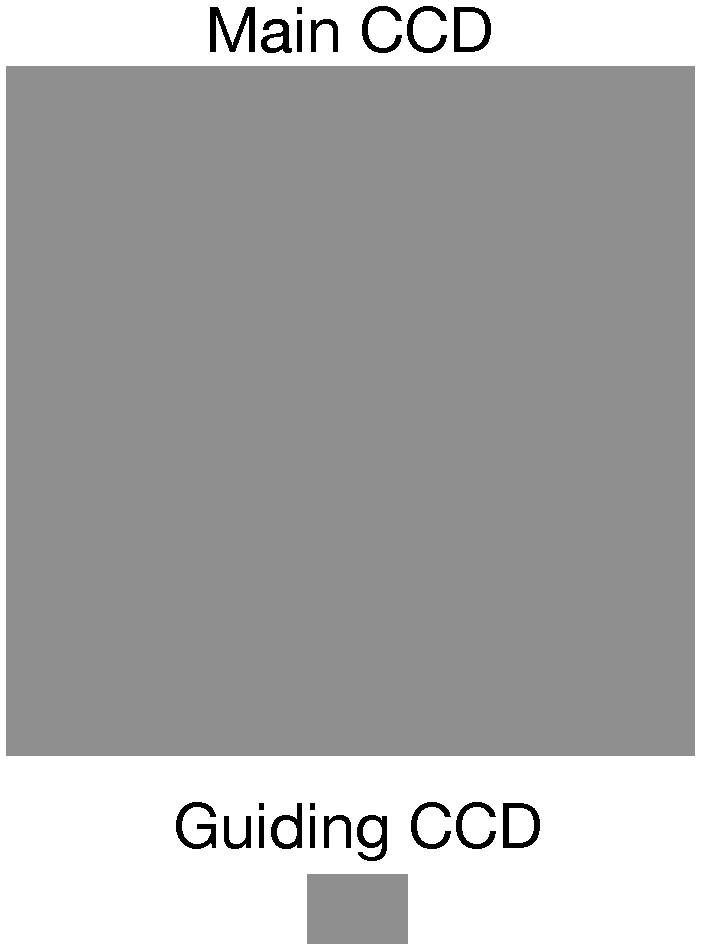
\includegraphics[width=0.25\textwidth]{guiding-chip-position}
    \caption{Approximate location and size of the guiding chip in relation to the main imaging chip.
        Note the small field of view of the guider.
    }
    \label{finder}
\end{figure}


% Add here: Stellarium screenshot of guider position and settings. maybe reference \ref{fig:NINA:}

To guide with the dual-chip guider using the Ha filter, which is the most challenging filter to guide with, use a guide star that is magnitude 11 or brighter to get an SNR of 15 with a guider exposure time of 15 seconds.

Move the FOV around in stellarium until you have such a guide star in the rectangle of the guider


\subsection{N.I.N.A. troubleshooting}

\paragraph*{Camera connection failed.} It can happen that the camera won't connect or show up while trying to connect. In that case, try to restart it by pulling its power cord and putting it back in. If this does not work, it might be broken and you have to contact the TA.

\paragraph*{All devices/presets are missing.} If you open N.I.N.A. and it looks like it is newly installed or has a different color scheme, it is possible that e.g. an update caused a different/default program configuration to be loaded. 

\begin{figure}
    \centering
    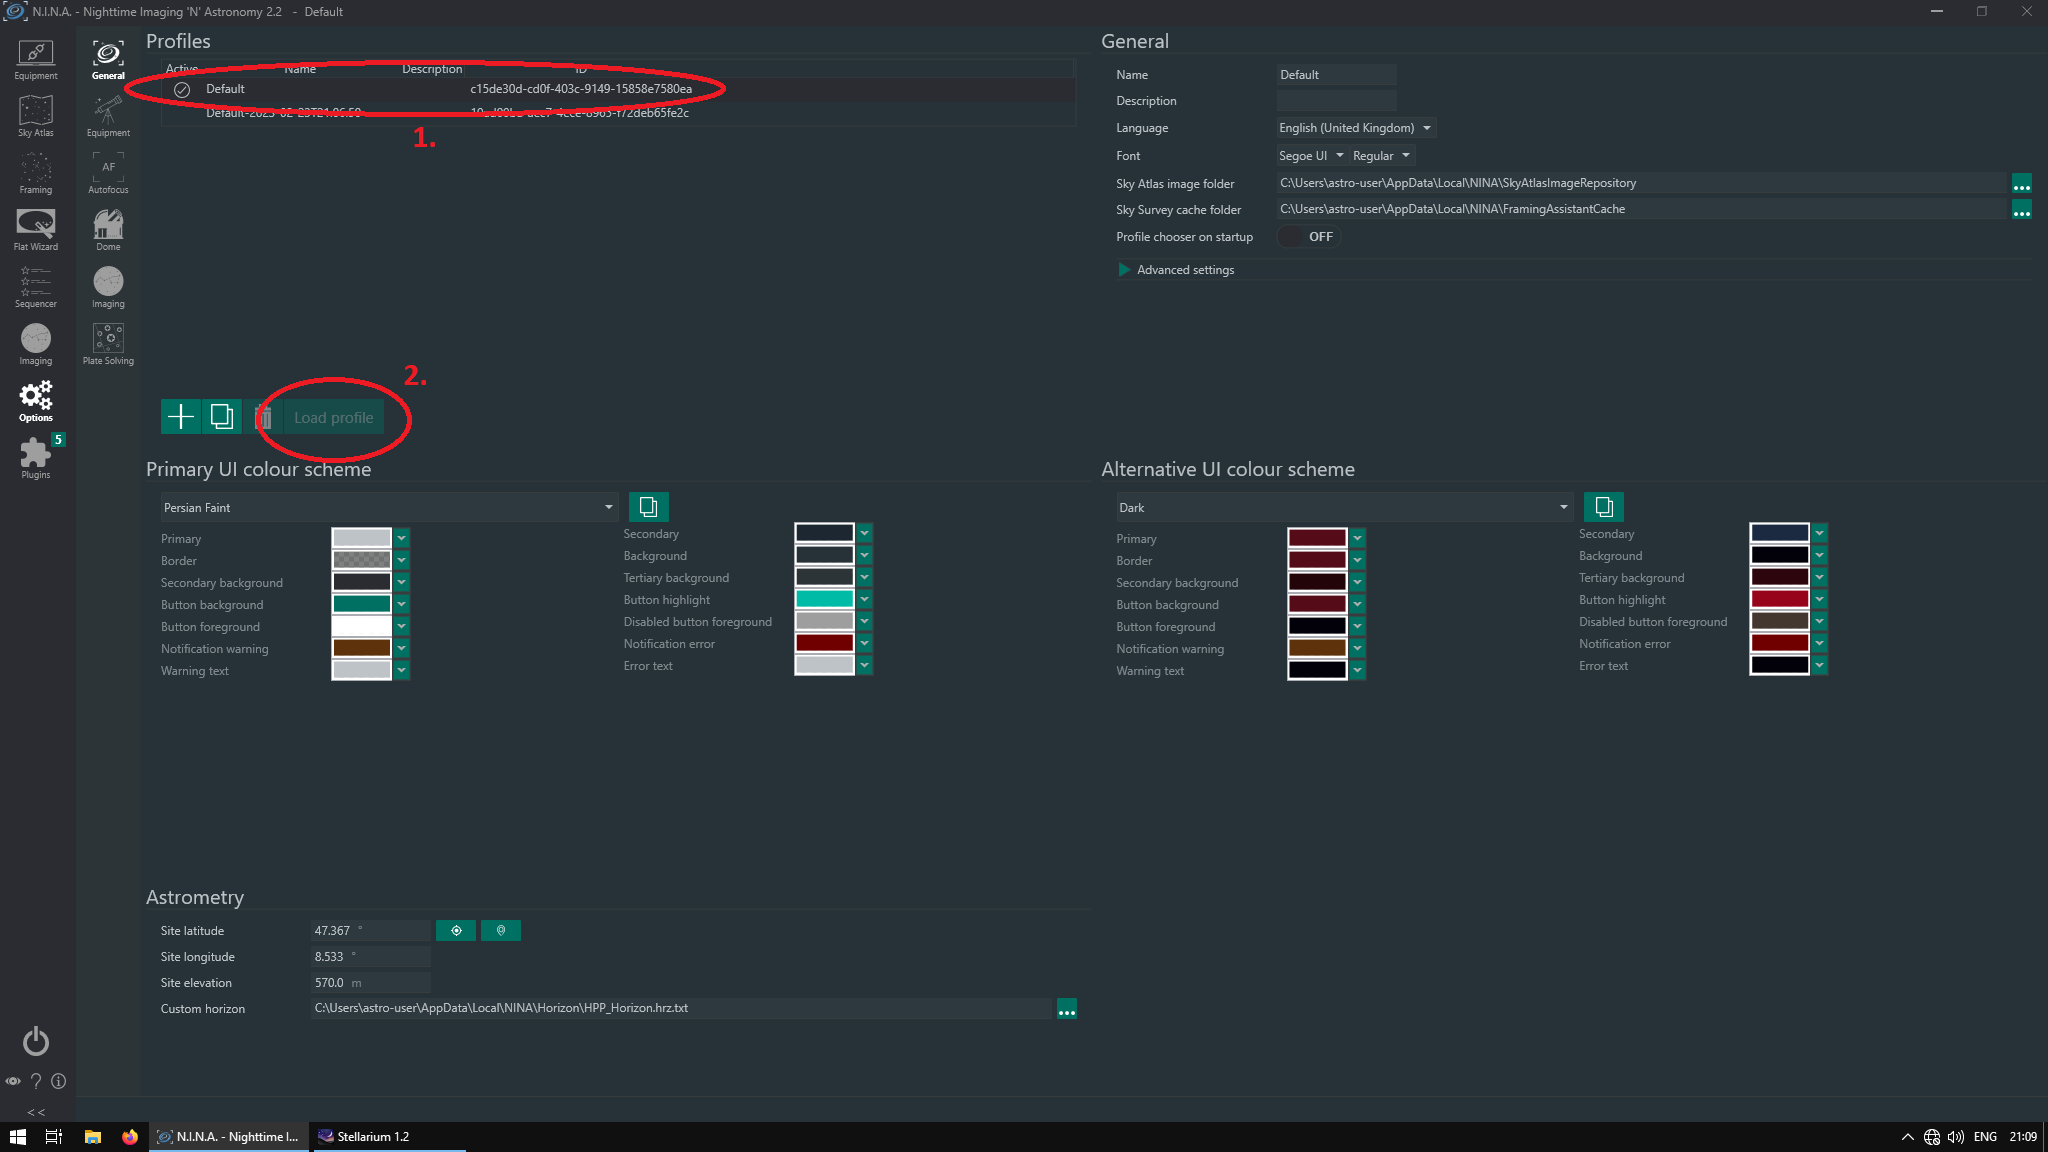
\includegraphics[width=0.85\textwidth]{figures/NINA/change_profile_edited.png}
    \caption{N.I.N.A. profile selection tab. The profile contains presets for loadable devices as well as lastly used focus values or filter configurations.}
    \label{fig:NINA:change_profile_edited}
\end{figure}

In order to select the right profile, make sure that all devices are disconnected. Then click on  \texttt{Options -> General} on the left bar. There you can select the right profile (as of June 2023) as displayed in 1. of \ref{fig:NINA:change_profile_edited}. If all devices are disconnected, you can then click on \texttt{Load profile} (2.) and the program will restart with the correct presets.



\subsection{Turn-off}

After usage, do not just leave the equipment, but turn everything off properly. In order to do so, you can follow the following steps. The terminology used is the same as in \ref{sec:NINA:start-up}. After making sure that every sequence is finished and changing to the \texttt{Equipment} tab on the left selection bar:

\begin{itemize}
    \item Select \texttt{Park} on the \texttt{Telescope} tab and wait until the telescope is done parking. You can verify that it is parked by looking outside or by noticing that ``\textit{Waiting for telescope to park}'' on the bottom left on the screen is not there anymore. Once it is parked, you can disconnect it by clicking on the disconnect button (such as 1. in figure \ref{fig:NINA:Telescope Connection}).
    \item Now click on \texttt{Filter Wheel} and disconnect it directly by clicking the disconnect button.
    \item Finally, click on \texttt{Camera}. First you have to turn off cooling by clicking on \texttt{Cancel} if it is active. Now wait until the telescope is again above $0\,\si{\degreeCelsius}$. If you want to speed up the process, activate \texttt{Warming} (and deactivate it once it is above $0\,\si{\degreeCelsius}$). Then you can disconnect the camera.
\end{itemize}

After everything is disconnected, you can simply close the program and shut down the computer(s). Now you can turn off the power to the hardware.



\section{PWI3: Heater and fans}
\texttt{PWI3} is usually only used for maintenance operations and can be ignored during normal imaging.
It can control the focusser, the mirror fans, the mirror heaters, and the temperature sensors.

Note that the focusser will overshoot its target and then correct itself when moving in one direction.
This is intentional, to avoid backlash errors caused by the gearing of the focus mechanism.

One useful feature is that you can recalibrate the Home position of the focusser, in case it ever refuses to move.

The best conditions for observation are when the ambient and the mirror temperatures have very similar values, but this requires a long time to be in place, therefore the observations are usually done without this prescription.

\section{MountWizzard4: Automatic telescope alignment}

\texttt{MountWizzard4} (MW4) is used to automatically align the telescope with the sky.
After completing an automatic alignment with MW4, you can expect the telescope to slew to a target with an error of only a few arcseconds, and you will be able to take long exposures without autoguiding.
(TBD how long.)

The mount model that MW4 builds will also account for the mechanical flexure of the mount and diffraction effects of the atmosphere.
When the atmosphere changes significantly, e.g. air pressure or temperature, you might want to re-run the automatic alignment in order to get optimal results.
However, it should be good enough for most purposes even without doing that.

Quick instructions:
% Install Python 3.10 (from Python website) and Mountwizzard4 from github.

\begin{enumerate}
    \item Change the filter to L in N.I.N.A., such that you can use fast exposure times during alignment.
          
          Then, you can close N.I.N.A.
    \item
          Open \texttt{Command Prompt}, and enter
          \begin{minted}{bash}
      cd Downloads\MountWizzard4
      startup.pyz
  \end{minted}
          After a few seconds, the software will open.
    \item
          Go to the \texttt{Settings} tab, and make sure that the camera driver is set to \texttt{ASCOM.
              HomeMade.SBIGImagingCamera}, and that the plate solve is set to \texttt{ASTAP}.
    \item
          Verfiy that in the top bar, at least the following three devices light up green: Mount, Camera, and Solver.
    \item
          Go to \texttt{Imaging -> Manage imaging train}, and verfiy the camera settings:
          \begin{itemize}
              \item
                    Exposure: 3s
              \item
                    Binning: 3
              \item
                    Subframe: \SI{100}{\percent}
              \item
                    Cooler Temp: \SI{-15}{\celsius}, and Cooler on
              \item
                    Use fast image download for modelling is on
          \end{itemize}
    \item
          Go to \texttt{Modelling -> Generate Build Points}
          \begin{itemize}
              \item
                    For a quick alignment, select \texttt{For Alignment}, and 6 points. (takeds a few minutes)
              \item
                    For a full model, select 95 points with a Golden Spiral. (takes one hour, usually not necessary)
          \end{itemize}
    \item
          Go to \texttt{Modelling -> Model Build and Program}, press \texttt{Run}.
    \item
          Wait until the process is finished.
          It can be monitored with the \texttt{Hemis} and \texttt{Message} windows.
    \item
          Go to \texttt{Modelling -> Manage Models} to inspect the new model.
          You can save it here.
    \item
          Set the model as active in the mount with the \texttt{Virtual keypad}.
\end{enumerate}

\chapter{Spectrography}

\section{Overview}

\section{Spectroscopy with the \textsc{dados} spectrograph}\label{spectroscopy}

\subsection{General comments}

Operation of the \textsc{dados} spectrograph has been tested successfully (see \cref{dados first light}), but the observing procedure has to be improved and the calibration strategy established.

Next steps:
\begin{itemize}
    \item determine approximate correlation between the \si{\um} screw positions and observed spectral region
    \item determine best focus positions for the Slitviewer-Webcam and the spectrum on the ST-1603 camera.
          \\ Note: use the calibration lamp and solar spectrum
    \item
          Improve and mark alignment of the Webcam with respect to the slits.
          In principle all slits fit onto the field-of-view of the webcam (see \cref{slits}).
          \\ Note: align the slits horizontally as in \cref{slits} for N-S
          and E-W movement of the target.
    \item
          align the spectrograph assembly and the ST-1603 camera to the telescope N-S /
          E-W movement of the target.
    \item
          observe different spectral standard stars at different pointing directions and
          test tracking quality for target on the slit.
    \item
          investigate manual tracking options. \\ Note: for very small pointing
          corrections of a few arcsec the mount first moves away a greater distance and
          then slowly comes back to the corrected position (compensation of gear-wheel
          errors).
          This is not practical for manual tracking corrections but it might be possible to switch-off or relax this setup for the mount.
    \item
          check whether it is more practical to use an external Webcam software (instead
          of MaxImDL) to simultaneously have the webcam and the telescope controls open
    \item
          establish full calibration procedure\\ Note: see \textsc{dados} tutorial by Bernd
          Koch from Baader planetarium \\
          (\url{http://www.baader-planetarium.de/dados/download/tutorial-dados-d.pdf})
    \item
          check impact of Barlow-Lens, i.e. check vignetting with/without lens.\\ Note:
          the spectrograph is optimized for F/10 but the telescope is F/6.8.
          The barlow lens should correct for that.
\end{itemize}

\begin{figure}[t!]
    \centering
    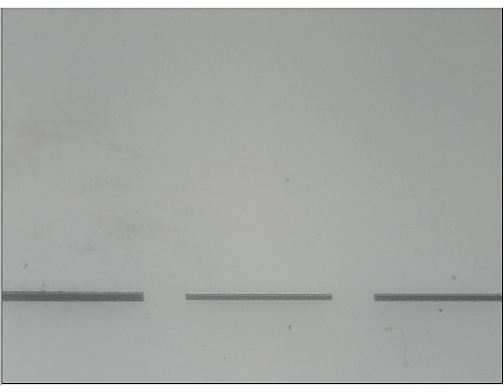
\includegraphics[width=0.47\textwidth]{slit-orientation}
    \caption{Optimized slit orientation on the webcam.}
    \label{slits}
\end{figure}

%=====================================
\subsection{Spectrograph assembly and setup}
%=====================================

See \cref{packing,dados telescope} for an overview of the packing of all the components and their, assembly for observation.
See \cref{dados calib} for the calibration assembly using the neon calibration lamp.
\\

The spectrograph consists of the following sub-parts:
\begin{itemize}
    \item \textbf{\textsc{dados} spektrograph}:\\ - 3 reflection gratings (200 L/mm, 900 L/mm, 1200 L/mm)\\ - 2 eyepieces + focus lens for using eyepieces as slit viewer - different adapter pieces for telescope and camera
    \item \textbf{Webcam} slit viewer + USB Extender-cable
    \item \textbf{ST-1603\textsc{ccd}camera}
    \item 1.5x \textbf{Barlow-lens} to extend telescope focal ratio of F/6.8 to $\sim$F/10
    \item \textbf{Neon calibration lamp}
    \item telescope adapter piece
\end{itemize}

\begin{figure}
    \centering
    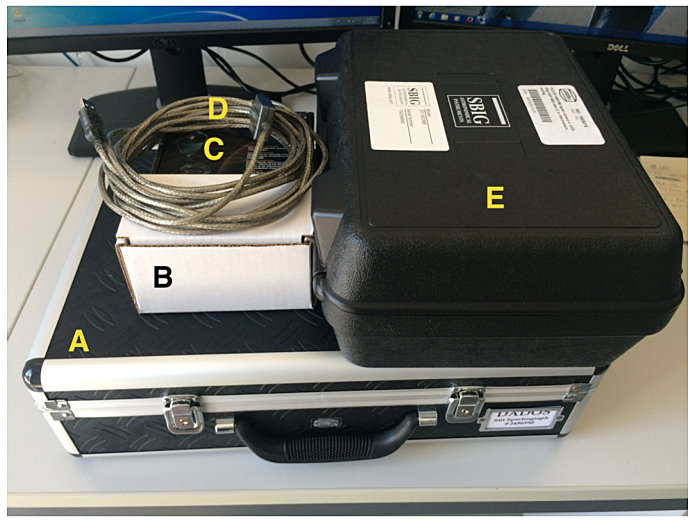
\includegraphics[width=0.47\textwidth]{dados-packing}
    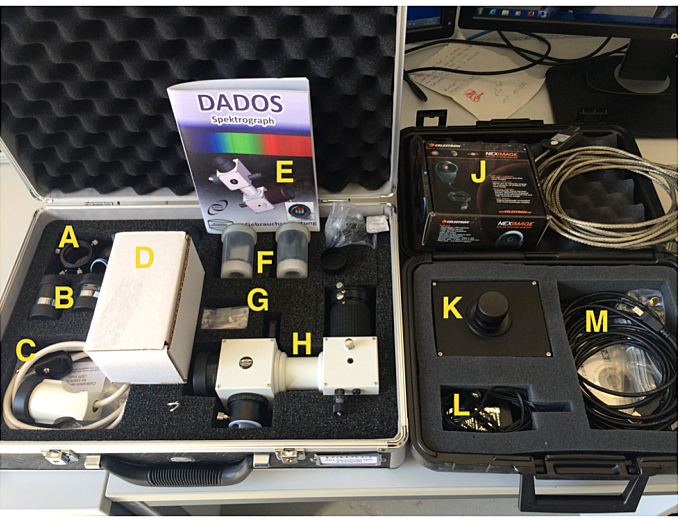
\includegraphics[width=0.47\textwidth]{dados-packing2}
    \caption{Spectrograph assembly: packing.
        \newline Top:\newline (A) \textsc{dados} case, (B) Barlow-lens, (C) Webcam, (D) USB Extender-cable, (E) ST-1603 case \newline Bottom:\newline (A) Mounting accessories, (B) Eyepieces, (C) Calibration lamp Neon, (D) Barlow-lens, \newline (E) \textsc{dados} manual, (F) additional Gratings, (G) \textsc{dados} tools, (H) \textsc{dados} spectrograph, \newline (J) Webcam, (K) ST-1603 CCD, (L) ST-1603 power cable, (M) ST-1603 accessories }
    \label{packing}
\end{figure}

\begin{figure}
    \centering
    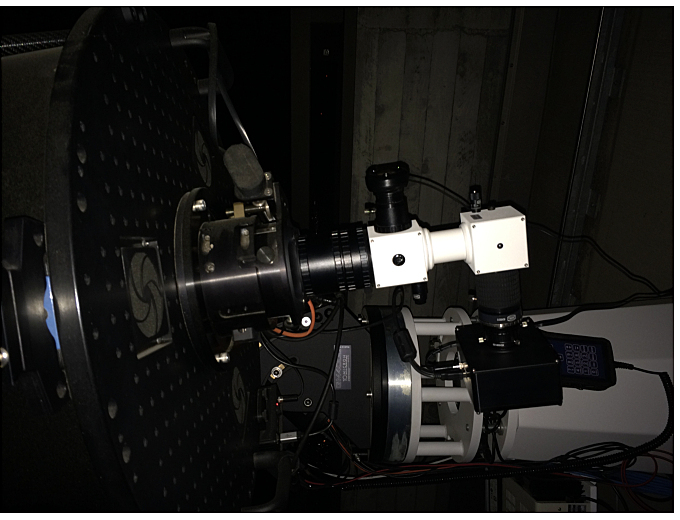
\includegraphics[width=0.47\textwidth]{dados-telescope}
    \caption{Spectrograph assembly attached to the telescope.  \newline Note: in this image the webcam is mounted 180 $^\circ$ opposite to the recommended position (see \cref{dados complete}).}
    \label{dados telescope}
\end{figure}

\begin{figure}[t!]
    \centering
    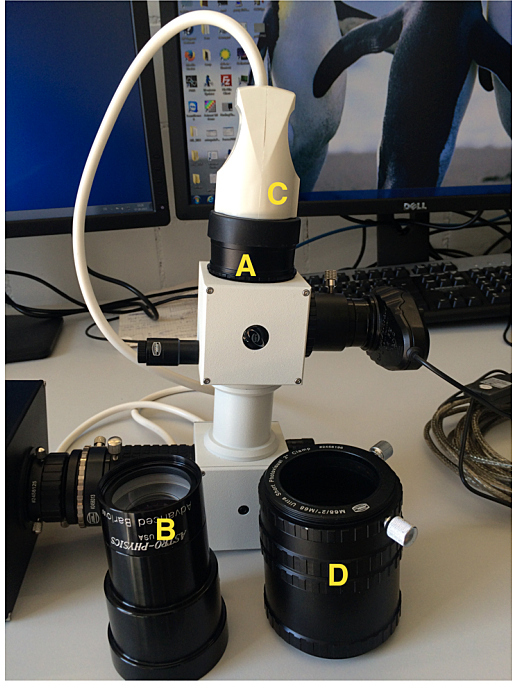
\includegraphics[width=0.47\textwidth]{dados-assembly-calib}
    \caption{Spectrograph calibration assembly:  \newline Replace the Barlow-lense by the 2'' receptacle and attach the Neon calibration lamp.
        Note: for storage of the Barlow-lens attach it to the barlow-lens adapter piece.
        \newline (A) 2'' receptacle, (B) Barlow-lens on adapter piece for storage, (C) Neon calibration lamp, \newline  (D) telescope adapter piece (not used for calibration) }
    \label{dados calib}
\end{figure}

For attachment to the telescope use the adapter piece as shown by \cref{dados complete}.
For the \textbf{\textit{Webcam}} use the USB-Extender cable and connect it to the remote telescope computer.
For the \textbf{\textit{ST-1603}} use the same USB-cable as for the \textit{STX-16803} which is already laid through the GM4000 mount and connected to the remote computer.
Connect the \textbf{\textit{ST-1603}} power adapter to the power outlet box belonging to the main power switch (see \cref{fig:main-switch}).
\\

\textbf{IMPORTANT: Always make sure that the webcam USB cable and the ST-1603 power cable cannot get stuck when moving the telescope!}\\

\textbf{IMPORTANT: Make sure that the Barlow-lens is tightly screwed into the \textsc{dados} spectrograph and that the complete spectrograph assembly is
    securely attached to the telescope and all the attachment screws are tight!}\\

\textbf{IMPORTANT: see \textsc{dados} manual for exchanging the gratings.
    Only exchange the gratings in a clean environment with electrostatic shielding!
    Use the optical gloves and never touch the gratings by hand!
}

\begin{figure}[t!]
    \centering
    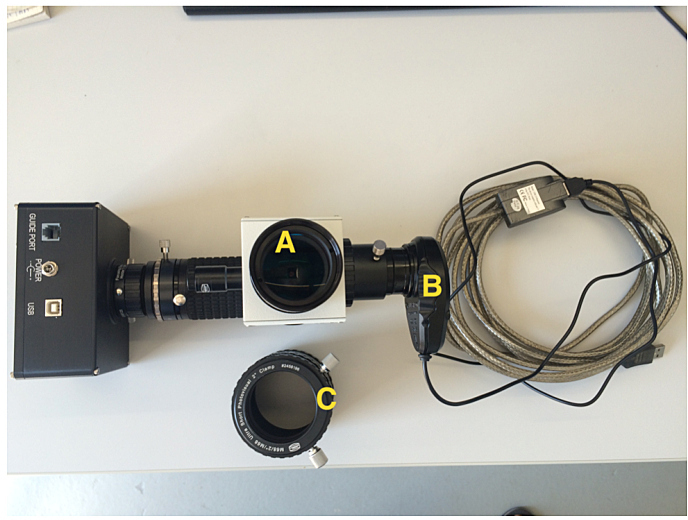
\includegraphics[width=0.47\textwidth]{dados-assembly-3}
    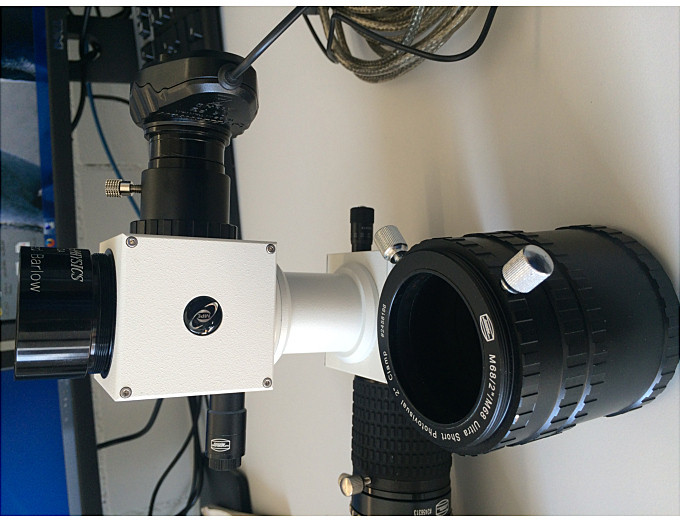
\includegraphics[width=0.47\textwidth]{dados-assembly-4}
    \caption{Spectrograph assembly:  \newline Complete assembly with attached Barlow-lens and Webcam ready to be attached to the telescope.
        Note that this webcam orientation will produce the slit-image as in \cref{slits}.
        The telescope adapter piece as shown is optimized for focusing the target onto the slit.
        \newline (A) Barlow-lens, (B) Webcam, (C) Adapter piece for telescope }
    \label{dados complete}
\end{figure}

%=====================================
\subsection{Alignment}\label{spectrograph alignment}
%=====================================

\subsubsection{Spatial orientation}

Attach the \textbf{\textit{ST-1603}} and the \textbf{\textit{Webcam}} with orientations as indicated by \cref{dados complete}.
This makes sure that all three slits are visible and horizontally oriented in the webcam (see \cref{slits}).
When attaching the \textbf{\textit{complete spectrograph assembly}} to the telescope make sure that it is oriented horizontal or vertical with respect to N-S / E-W.
This makes it easier to move the target onto the slit using the telescope N-S/E-W keys.
\\

\textbf{Important: Before attaching the spectrograph assembly to the telescope make sure that the focal alignment is done (using the calibration lamp, see next Section)!}

\subsubsection{Focal alignment}

The focal alignment needs to be done off the telescope using the \textbf{\textit{slit illumination}} and the \textbf{\textit{Neon calibration lamp}}:\\

\textbf{A) slits on Webcam:}
\begin{itemize}
    \item turn on the \textbf{\textit{slit illumination}} (see \cref{dados main}).
    \item
          \textbf{\textit{focus the slits}} onto the webcam by moving the webcam in/out.\\
          i.e. the slit-image should look similar to \cref{slits} or better
    \item
          tightly fix the webcam position
    \item
          turn off the slit illumination
\end{itemize}

\textbf{B) spectrum on ST-1603:}
\begin{itemize}
    \item
          Attach the \textbf{\textit{calibration lamp}} to the spectrograph assembly
          according to \cref{dados calib}.\\ i.e. replace the Barlow-lens by the 2''
          receptacle to attach the lamp
    \item
          loosen the \textbf{\textit{Focuser fixation screw}} (see \cref{dados main})
    \item
          start continuous imaging by the ST-1603 camera
    \item
          \textbf{\textit{focus the Neon spectrum}} onto the ST-1603 camera by using the camera Focuser of the \textsc{dados} spectrograph.
          (see Figs.~\ref{dados main}, \ref{neon spectrum})
    \item
          tighten the Focuser fixation screw
    \item
          detach the calibration lamp and re-attach the Barlow-lens
\end{itemize}

\textbf{Important: Also make sure that the spatial orientation of the webcam, the camera, and the complete spectrograph assembly is correct (see previous Section)!}

\begin{figure}[t!]
    \centering
    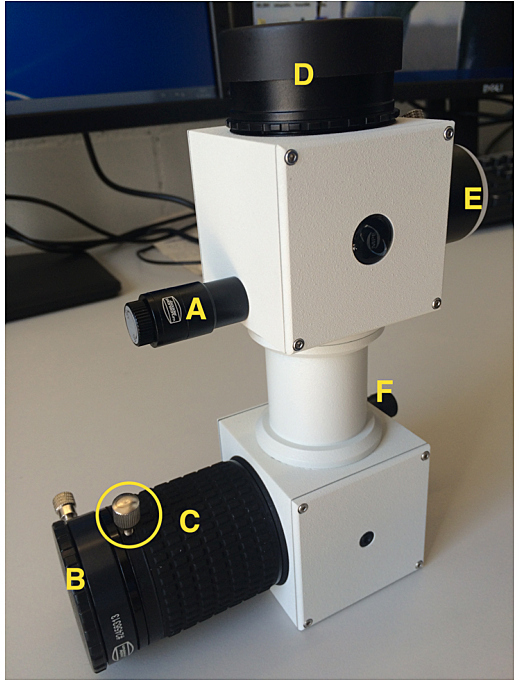
\includegraphics[width=0.47\textwidth]{dados-assembly-1}
    \caption{Spectrograph assembly: \textsc{dados} spectrograph. \newline (A) Slit illumination, (B) towards ST-1603, (C) Focuser for ST-1603 with fixation screw (circle), (D) towards telescope, (E) Slit viewer,  (F) \si{\um} screw for grating position }
    \label{dados main}
\end{figure}

\begin{figure}[t!]
    \centering
    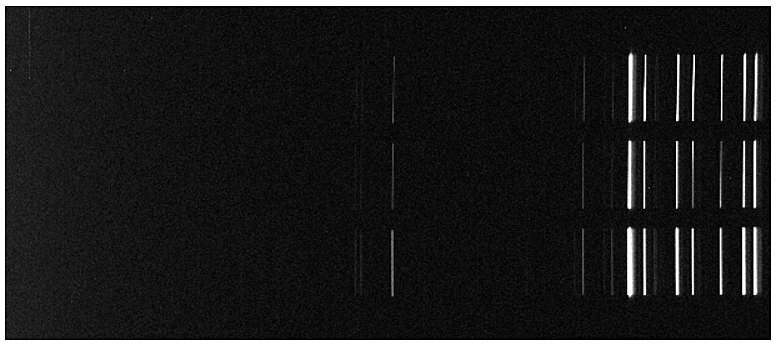
\includegraphics[width=0.47\textwidth]{neon}
    \caption{Neon calibration spectrum.}
    \label{neon spectrum}
\end{figure}

%=====================================
\subsection{Operation}
%=====================================

All sub-components required for the operation of the Spectrograph (i.e. the telescope, the ST-1603\textsc{ccd}camera, and the Webcam) are controlled by MaxImDL.
See Section~\ref{operation maximdl} for operational instructions for the telescope and the\textsc{ccd}camera.
In particular note how to setup and connect the ST-1603:\\

\textbf{Important: When using the ST-1603 camera set \textit{Filter or Controlling Camera Model} to \textit{No Filter}!
}\\

\textbf{Important: for the ST-1603 \textit{Subframe} does not work and needs to be de-activated!}\\

The webcam is also connected by the \textbf{Observatory} window (e.g. see \cref{fig:observatory_setup}) and operated by the \textbf{Webcam} tab (see \cref{operation webcam}).
\\

\textbf{General operation procedure}:
\begin{itemize}
    \item
          slew telescope to target
    \item
          if required: \textbf{focus target} onto slit focal plane imaged by ST-1603 by
          using the \textbf{MaxImDL Focus} tab.\\ - when using telescope adapter piece as
          in \cref{dados complete} focus position $\sim24913~\mu$m (\textbf{TBC})
    \item
          \textbf{center target onto desired slit} by using the N-S/E-W buttons of the telescope control (see
          Figs.~\ref{fig:observatory_telescope}, \ref{operation webcam}):\\
          - select step size 10 Sec. or less\\
          - if required turn On/Off slit illumination
    \item
          turn Off slit illumination
    \item
          \textbf{acquire spectrum} with ST-1603 (see \cref{spectrum})
    \item
          change spectral range by using the grating $\mu$m screw (see \cref{grid-position} and comments therein)
    \item
          check target-slit alignment
    \item
          \textbf{acquire spectrum} with ST-1603
    \item
          change spectral range by using the grating $\mu$m screw
    \item
          check target-slit alignment
    \item
          \textbf{acquire spectrum} with ST-1603
    \item
          ...
\end{itemize}

\begin{figure}[t!]
    \centering
    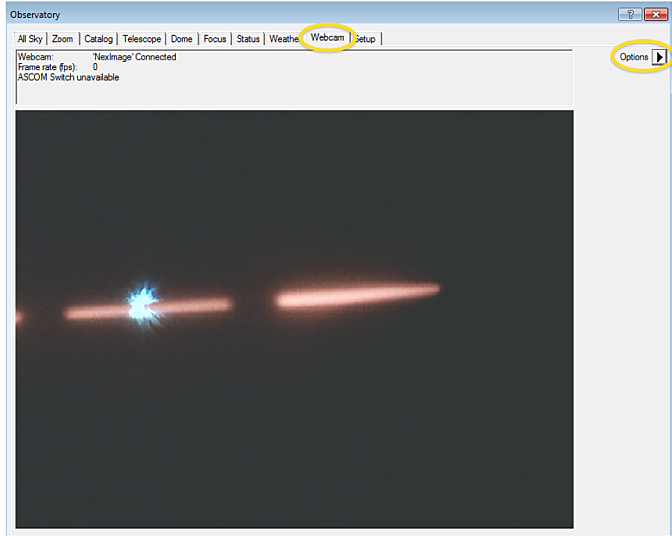
\includegraphics[width=0.47\textwidth]{dados-operation-webcam1}
    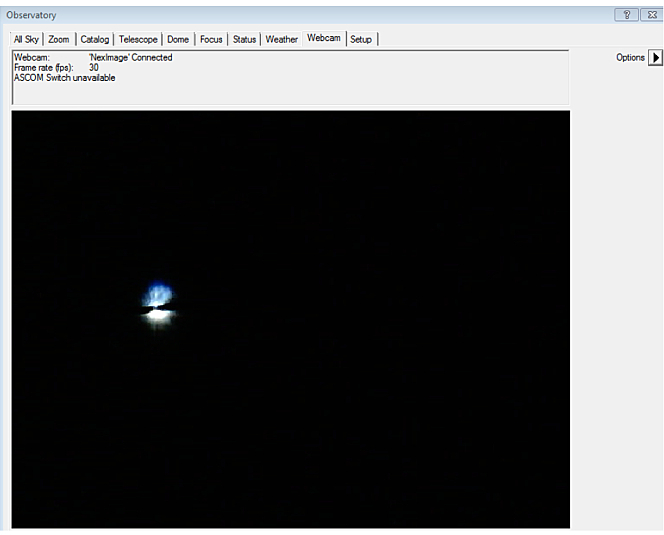
\includegraphics[width=0.47\textwidth]{dados-operation-webcam2}
    \caption{Webcam operation with \textbf{\textit{slit illumination}
            On} (top) and \textbf{Off} (bottom).
        Settings for the webcam are accessible by the \textbf{\textit{Options}} button.
        \newline Note that in these images the webcam orientation is not in the recommended position (see Figs.~\ref{dados complete}, \ref{slits})}
    \label{operation webcam}
\end{figure}

\begin{figure}[t!]
    \centering
    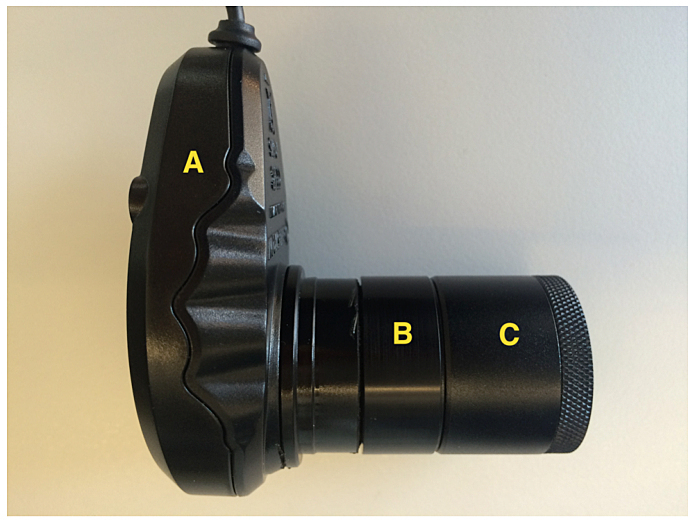
\includegraphics[width=0.47\textwidth]{webcam}
    \caption{Spectrograph assembly: Webcam  \newline The webcam has been modified by an adapter peace to attach the slit-viewer focusing lens. \newline (A) Webcam, (B) adapter piece, (C) Focusing lens.}
    \label{webcam}
\end{figure}

\begin{figure}[t!]
    \centering
    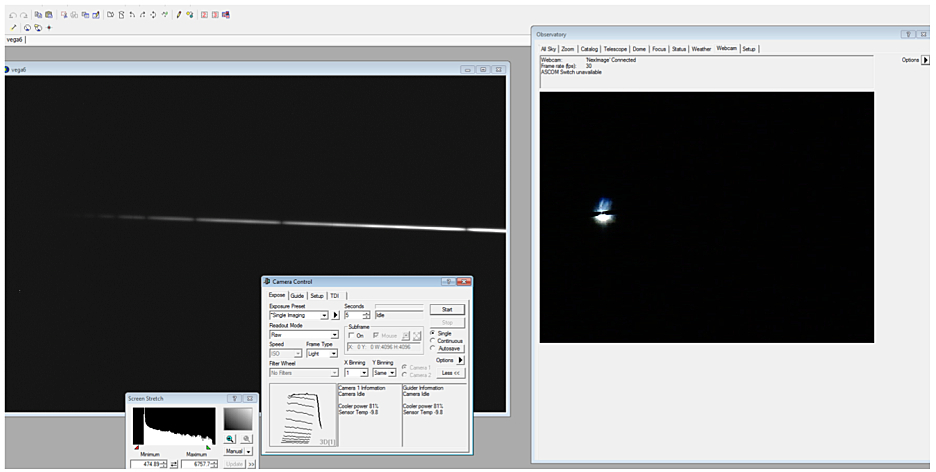
\includegraphics[width=0.47\textwidth]{spectrum}
    \caption{Commissioning image of Vega spectrum. \newline Note that in this image the webcam and spectrograph assembly orientation are bad.
        For the recommended orientations see Sect.~\ref{spectrograph alignment} and Figs.~\ref{dados complete}, \ref{slits}.
    }
    \label{spectrum}
\end{figure}

\begin{figure}[t!]
    \centering
    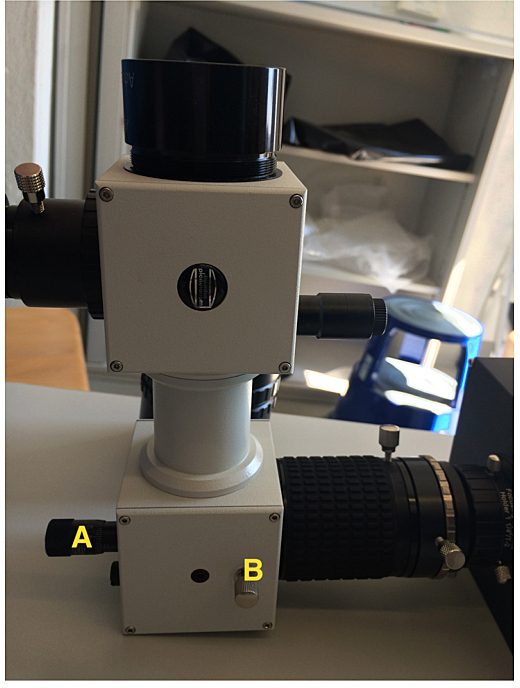
\includegraphics[width=0.47\textwidth]{dados-grid-position}
    \caption{Changing the grating position to change the spectral range:  \newline Loosen the fixation screw (but do not completely remove it!) and use the
        \si{\um} screw to change the illumination angle of the grating.
        Note that pushing the grating (
        \si{\um} screw goes in) works better than pulling (push fixation screw sideways to support pulling the grating with
        \si{\um} screw): \newline (A)
        \si{\um} screw, (B) fixation screw } \label{grid-position}
\end{figure}

\subsection{Calibration (TBD)}

\textbf{ TBD\\ } see also \url{http://www.baader-planetarium.de/dados/download/tutorial-dados-d.pdf}

\section{First light of \textsc{dados} spectrograph}\label{dados first light}

\begin{figure}[H] \centering 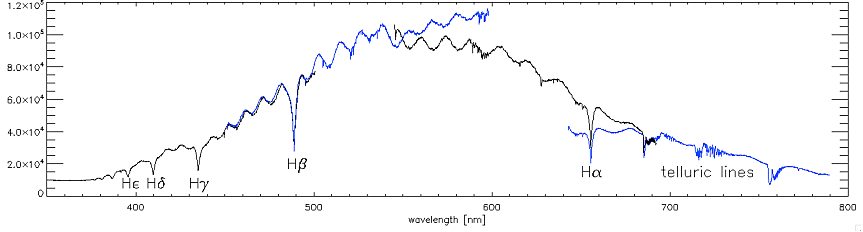
\includegraphics[width=12cm]{vega_spectrum_uncalibrated} \caption{Uncalibrated Vega spectrum using the 900 L/mm grating.
        %=====================================%=====================================
        \newline The different spectral regions are not calibrated but simply scaled to match each other.
        The plate scale is $\sim$ 0.096~nm/pixel which was determined using the solar spectrum and the Neon calibration spectrum.
    }
    \label{vega uncalibrated}
\end{figure}

\begin{figure}[H]
    \centering
    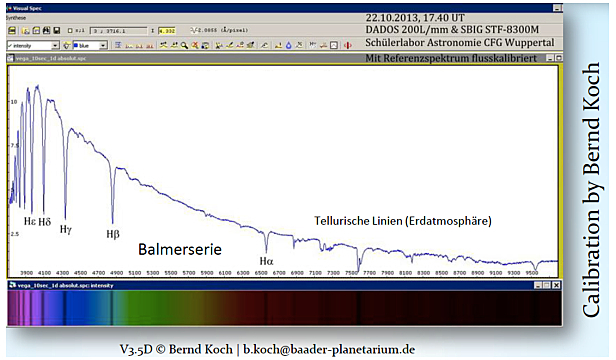
\includegraphics[width=12cm]{vega_koch}
    \caption{As comparison to our uncalibrated first light spectrum (\cref{vega uncalibrated}): \newline Flux calibrated Vega spectrum by \textbf{Bernd Koch: \textsc{dados}
            Tutorial Baader Planetarium} (\url{http://www.baader-planetarium.de/dados/download/tutorial-dados-d.pdf}).
    }
    \label{vega calibrated}
\end{figure}

\part{Data analysis}

\chapter{Data Reduction}

Based on version 1.1 of the manual by Luca Tortorelli\autocite{Tortorelli2015_DataReduction}.
This part of the manual is intended to give a brief overview on how to go from the raw images to the fully astrometrically and photometrically calibrated ones.

\section{Software installation}

The data reduction is performed mostly in \software{Python}, but additional software may be required such as \software{ds9}, \software{Source Extractor}, \software{SCAMP}, \software{SWARP} and/or \software{DeepSkyStacker} and \software{IRIS} (the last two if you use Windows).


\subsection{DS9}

DS9 displays FITS images and it can be download and installed for all the platforms from \url{http://ds9.si.edu/site/Download.html}.

\subsection{Source Extractor}

\textbf{MacOS} users can easily install Source Extractor with 'brew' or 'Macports'.
However remember that you must have your virtual environment deactivated when you use 'brew' or 'Macports'.
In your terminal, run
\begin{minted}{bash}
    brew install homebrew/science/sextractor
\end{minted}
or
\begin{minted}{bash}
    brew install brewsci/science/sextractor
\end{minted}
since sometimes packages change directory.
If you want to install it with Macports, then first you have to install it according to your operating system \url{https://www.macports.org/install.php}.
Then simply type in your terminal:
\begin{minted}{bash}
    sudo port install sextractor
\end{minted}

For \textbf{Linux} users, the simplest way to have SExtractor up and running is to install the standard binary package the comes with your Linux distribution.
Run, e.g.,
\begin{minted}{bash}
    apt-get sextractor
\end{minted}
(on Debian) or
\begin{minted}{bash}
    dnf sextractor
\end{minted}
(on Fedora) as root and SExtractor, as well as all its dependencies, will automatically be installed.
Alternatively, you can follow the instructions at \url{https://sextractor.readthedocs.io/en/latest/Installing.html}.

Source Extractor can't be installed on \textbf{Windows}.
In Windows 10, however, you can activate the Unix terminal.
Maybe there it works, but I have never tested it.

The instructions on how to use it are at \url{https://sextractor.readthedocs.io/en/latest/Using.html}.

\subsection{SCAMP}

SCAMP computes the astrometric solution of astronomical images.
Since I provide also a website where to do it, it is not stricly necessary that you install it.

\textbf{MacOS} users can easily install SCAMP with 'Macports'.
Simply type
\begin{minted}{bash}
    sudo port install scamp
\end{minted}
in your terminal window.

\textbf{Linux} users have to follow the instructions on the website \url{https://scamp.readthedocs.io/en/latest/Installing.html}.

SCAMP can't be installed on \textbf{Windows}.
In Windows 10, however, you can activate the Unix terminal.
Maybe there it works, but I have never tested it.

\subsection{SWARP}

\textbf{MacOS} users can easily install SWARP with 'Macports'.
Simply type
\begin{minted}{bash}
    sudo port install swarp
\end{minted}
in your terminal window.

\textbf{Linux} users have to follow the instructions on the website \url{https://www.astromatic.net/software/swarp}.

SWARP can't be installed on \textbf{Windows}.
In Windows 10, however, you can activate the Unix terminal.
Maybe there it works, but I have never tested it.

\subsection{DeepSkyStacker}

DeepSkyStacker performs the same steps as SWARP, but with a graphical interface.
It works only on \textbf{Windows} (Mac or Linux users may try using it via Wine) and it can be downloaded at \url{http://deepskystacker.free.fr/english/index.html}.
The website containes several tutorials on how to use it.

\subsection{IRIS}

IRIS is an astronomical images processing software that works under Windows OS.
It can be used to perform the analysis steps highlighted in Section \ref{section:data_red_steps}.
The website to download it is \url{http://www.astrosurf.com/buil/iris-software.html}.
This page contains several tutorials on how to use it for different astronomical applications.

\section{Data Reduction Steps}
\label{section:data_red_steps}

In this section we go through the different data reduction steps, with some example code on how to perform the different tasks.
The code can be run either in the terminal or inside a Jupyter notebook.
Some glossary: 'raw science frame' refers to a single exposure image of the target galaxy or star without any post-processing applied to it, i.e. as it is taken at the telescope; 'dark for flat' refers to a dark image taken with the same exposure time as the single flat field image, while 'dark for science' refers to a dark image taken with the same exposure time as the 'raw science frame'.

\subsection{Dark Subtraction and Flat Fielding Correction}

The bias, dark subtraction and the flat fielding correction are applied to the 'raw science frame' according to the following:
\begin{equation}
    \mathrm{science\ frame} = \frac{\mathrm{raw\ science\ frame} - \mathrm{master\ dark} }{\mathrm{master\ flat} / \left \langle \mathrm{master\ flat} \right \rangle} \label{correction}
\end{equation}
`science frame' refers to the `raw science frame' after bias, dark subtraction and flat fielding correction.
`master bias' refers to the median image of all the bias frames. 'master dark' refers to the median image of all the 'dark for science' images, the latter being subtracted for the `master bias'. 'master flat' refers to the median image of all the flat images after 'dark for flats' subtraction and `master bias' subtraction. $ \left \langle \mathrm{master\ flat} \right \rangle$ is the mean value of the 'master flat' image.

Images can be read with the \software{astropy} package.
In the terminal, type
\begin{minted}{python}
    from astropy.io import fits
    data = fits.getdata('path_to_image', ext=0)
    head = fits.getheader('path_to_image', ext=0)
\end{minted}
to get the electronic counts in each pixel and the metadata (header file) of an image.
The 'data' variable stores the image in the form of a 2D array (i.e. a matrix), therefore operations such as sum, difference, ratio etc. can be done simply as
\begin{minted}{python}
    diff = data1 - data2
\end{minted}

In order to create a median image, you can for example store each 'data' variable for each image as element of a list or create a 3D array having size as the number of images times the number of pixels for each side of the image.
Then you simply run
\begin{minted}{python}
    import numpy as np
    median_image = np.median(image_list, axis=0)
\end{minted}
The variable 'median image' will contain the median of the electronic counts of the different images pixels.
To create an image that can be displayed also in DS9, run
\begin{minted}{python}
    fits.writeto('out_image_path', median_image, head, overwrite=True)
\end{minted}

Once you create the different median images, you can perform the dark subtraction and the flat fielding corrections as in \ref{correction}.

An alternative way of performing this data reduction tasks is by using IRIS.
One needs to follow the tutorial in \url{http://www.astrosurf.com/buil/iris/tutorial3/doc13_us.htm} adapting it to our case.
First, select the image file format from the \textit{Settings} command of \textit{File} menu as FIT (see figure 1 in \url{http://www.astrosurf.com/buil/iris/tutorial3/doc13_us.htm}) and set the working path as the one where you store your images.
Then, you create a master bias, a master dark and a master flat following the sections `Create the master Offset image', `Create the master Dark image', `Create the master Flat-field image' in \url{http://www.astrosurf.com/buil/iris/tutorial3/doc13_us.htm}.
IRIS allows you also to create a bad pixel map for the image following the section `Create a pixel bad list'.
The bias, dark subtraction and flat field normalization is performed following the section `Preprocessing' in \url{http://www.astrosurf.com/buil/iris/tutorial3/doc13_us.htm}.
Further information can be found also in \url{http://www.astrosurf.com/buil/iris/tutorial2/doc8_us.htm} and \url{http://www.astrosurf.com/buil/iris/tutorial2/doc9_us.htm}.

\subsection{Cosmic Ray Rejection}

The cosmic ray rejection can be performed with Astroscrappy\footnote{\url{https://github.com/astropy/astroscrappy}} or \software{cosmics.py}\footnote{\url{https://obswww.unige.ch/~tewes/cosmics_dot_py/}}.

\paragraph{\software{Astroscrappy}}
The syntax for Astroscrappy is the following:
\begin{minted}{python}
    from astroscrappy import detect_cosmics
    from astropy.io import fits
    data = fits.getdata('path_to_image', ext=0)
    head = fits.getheader('path_to_image', ext=0)
    mask, _clean = detect_cosmics(data, inmask=None, sigclip=4.0, sigfrac=0.3, objlim=5.0, gain=1.15, readnoise=6.5, satlevel=65536, pssl=0.0, niter=4, sepmed=True, cleantype='meanmask', fsmode='median', psfmodel='gauss', psffwhm=2.5, psfsize=7, psfk=None, psfbeta=4.765, verbose=False)
    fits.writeto('path_to_image_cr.fits', _clean, head, overwrite=True)
\end{minted}
The values as just for reference.
Read the documentation and figure out by yourself the correct ones.
Gain can be read from the header of each image, while saturation and readout noise can be found in the\textsc{ccd}camera manual.

\paragraph{\software{cosmics.py}}
\begin{minted}{python}
    import cosmics
    data = fits.getdata('path_to_image', ext=0)
    head = fits.getheader('path_to_image', ext=0)
    c = cosmics.cosmicsimage(gal_raw, gain=1.15, readnoise=0, sigclip = 5.0, sigfrac = 0.3, objlim = 5.0, satlevel=65535)
    c.run(maxiter = 4)
    cosmics.tofits('path_to_image_clean.fits', c.cleanarray, head)
\end{minted}
The values as just for reference.
Read the documentation and figure out by yourself the correct ones.
Gain can be read from the header of each image, while saturation and readout noise can be found in the \textsc{ccd} camera manual.

IRIS performs the same tasks by creating a bad pixel map for the image following the section `Create a pixel bad list' in \url{http://www.astrosurf.com/buil/iris/tutorial3/doc13_us.htm} or following the section `Manual hot-spot removal procedure' in \url{http://www.astrosurf.com/buil/iris/tutorial8/doc23_us.htm}.

\subsection{Background Subtraction}

The background subtraction can be performed using 'phoutils'.
First you estimate the background following \url{https://photutils.readthedocs.io/en/stable/background.html} for every 'science image'.
Then you subtract the background image from each science image.
Have a look at the image after background subtraction, the process is not trivial and you have to play with parameters in order to obtain a good result.

An example code for a 1D background subtraction is the following:
\begin{minted}{python}
    data = fits.getdata('path_to_image', ext=0)
    head = fits.getheader('path_to_image', ext=0)
    mask = make_source_mask(data, snr=2, npixels=5, dilate_size=11)
    mean, median, std = sigma_clipped_stats(data, sigma=4.0, mask=mask)
    backsub_data = data - mean
    fits.writeto('path_to_image_backsub.fits', backsub_data, head, overwrite=True)
\end{minted}

The background subraction can be performed with IRIS following the section `The final touch' in \url{http://www.astrosurf.com/buil/iris/tutorial2/doc8_us.htm}.

\subsection{Astrometric Calibration}

The astrometric calibration is performed through the website \url{astrometry.net}.
You need to upload either a single image or a tarball (.tar, .gz), containing fits images to \url{http://nova.astrometry.net/upload}.
It will recognize stars in the image and it will give you back the same input images, but with the astrometric solution included.

The same steps can be performed using SCAMP.
See \url{https://scamp.readthedocs.io/en/latest/Using.html} for a tutorial on how to use it.
SCAMP needs a list of catalogues and a configuration file in order to work.
First, you need to run Source Extractor on each image.
Look for the 'default.param' file and uncomment the lines containing the following parameters: 'XWIN\_IMAGE', 'YWIN\_IMAGE', 'ERRAWIN\_IMAGE', 'ERRBWIN\_IMAGE', 'ERRTHETAWIN\_IMAGE', 'FLUX\_AUTO', 'FLUXERR\_AUTO', 'FLAGS', 'FLAGS\_WEIGHT', 'IMAFLAGS\_ISO', 'FLUX\_RADIUS', 'ELONGATION'.
The, look for the 'defaul.sex' file, open it and change 'CATALOG\_TYPE' in 'FITS\_LDAC' and 'PARAMETERS\_NAME' in the path to 'default.param'.
The rest of the parameters is up to you to discover what they do and which value to choose.
Now you can run Source Extractor:
\begin{minted}{bash}
    sex image_path -c default.sex -CATALOG_NAME 'path_to_catalogue_name'
\end{minted}
These catalogues that you have created for each image will be read by SCAMP.
First, create an ASCII file where each line contains the path to the Source Extractor output catalogues, preceded by \@.
Then look for the configuration file (usually it ends with '*.conf') and check that the 'SOLVE\_ASTROM' parameters is set to 'Y'.
Check the manual for the other parameters meaning and values.
Then run SCAMP with
\begin{minted}{bash}
    scamp catalogue_list -c scamp.conf
\end{minted}

Alternatively, you can use a \software{Python} package called 'astroalign' (\url{https://github.com/toros-astro/astroalign}).
You can install it with
\begin{minted}{bash}
    pip install astroalign
\end{minted}
This package finds similar 3 point asterisms in an input and reference image and computes the affine transformation between them.
It may not work on images of extended objects with few point-like sources or in very crowded fields.
However, also in these cases, one of the three methods will do the job.
An example code is
\begin{minted}{python}
    from astropy.io import fits
    import astroalign
    data = fits.getdata('path_to_image', ext=0)
    reference_img = fits.getdata('path_to_ref_image', ext=0)
    reference_head = fits.getheader('path_to_ref_image', ext=0)
    aligned_image = astroalign.register(data, reference_img)
    fits.writeto('path_to_aligned_image.fits', aligned_image, reference_head, overwrite=True)
\end{minted}

IRIS contains a tool to perform astrometric calibration.
You can follow the tutorial in \url{http://www.astrosurf.com/buil/iris/tutorial13/doc31_us.htm}.

\subsection{Stacking}

Stacking consists of combining several astronomical images.
In order to do that, images have to be aligned one respect to each other.

There are 3 options to perform this task:
\begin{itemize}
    \item DeepSkyStacker: it has a graphical interface that makes things easy to perform, however it works only under Windows.
          Tutorials on how to use it can be found in the website.
    \item
          IRIS: first you need to align the single exposures.
          To do that, just follow the section `Align the images' in \url{http://www.astrosurf.com/buil/iris/tutorial3/doc13_us.htm} or follow the tutorials in \url{http://www.astrosurf.com/buil/iris/tutorial2/doc10_us.htm} or \url{http://www.astrosurf.com/buil/iris/tutorial2/doc11_us.htm}.
          After the alignment, you can stack the single exposure by following the section `Stack a set of images' in \url{http://www.astrosurf.com/buil/iris/tutorial3/doc13_us.htm} or follow the tutorial in \url{http://www.astrosurf.com/buil/iris/tutorial2/doc121_us.htm}.
    \item
          \software{Python}-based: first you align all the images to a reference one with 'astroalign'.
          Then those images can be combined by adding them
          \begin{minted}{python}
            final_science = aligned_image_1 + aligned_image_2
          \end{minted}
          if you want to obtain a deeper image (e.g., for galaxies), or they can be combined by averaging them
          \begin{minted}{python}
            list = [aligned_image_1, aligned_image_2]
            final_science = np.mean(list, axis=0)
          \end{minted}
          for example when you have star images, e.g., a standard star.
          This method does not work for images downloaded from 'astrometry.net', since it only computes the astrometric solution, but it doesn't change the pixel position of objects.
    \item
          SWARP: this is the most precise method, but it requires images having the
          astrometric solution in their headers.
          Therefore, it requires as input images downloaded from 'astrometry.net' or that have been processed with SCAMP.
          SWARP manual can be found at \url{https://www.astromatic.net/pubsvn/software/swarp/trunk/doc/swarp.pdf}.
          Look for the configuration file (it should end with '*.swarp') and check that the 'COMBINE' parameter is set to 'Y'.
          Check the manual for the other parameters meaning and values.
          If you have images from 'astrometry.net', you can create an ASCII file with image paths (as in SCAMP) and then you run SWARP with
          \begin{minted}{bash}
            swarp image_list -c hpp.swarp
          \end{minted}
          to obtain as output a coadded (combined) image.
          Exposure times, gains etc. will be updated accordingly.
          If you have catalogues from SCAMP, then it will output a .head file that can be read by SWARP by setting the 'HEADER\_ONLY' parameter to 'Y' (see manual for more details).
\end{itemize}

\subsection{Photometric Calibration}

The photometric zero-point $m_\text{ZP}$ of an image is defined as
\begin{equation}
    \label{eq:magnitude-zero-point}
    m = -2.5 \log_{10} \left( \frac{N}{t} \right) + m_\text{ZP},
\end{equation}
where $N$ is the number of counts (either photons or ADUs) of a source, $t$ is the exposure time, $m$ is the apparent magnitude of the source, and $m_\text{ZP}$ is the photometric zero-point of the image.
Here, it does not matter whether one uses ADUs or photons for $N$, as long as the same units are used for both the unkown source and the standard star.



Photometric calibration involves two steps:

First, a standard star with known magnitude $m$ is observed, and the number of counts $N$ is measured. Then, $m_\text{ZP}$ can be computed from \cref{eq:magnitude-zero-point}.
To measure the number of counts in a region, you can use \texttt{astropy}'s \texttt{photutils}\footnote{\url{https://photutils.readthedocs.io/en/stable/aperture.html}} package.

Then, a source with unknown magnitude $m$ is observed, and its number of counts $N$ is measured. Using the magnitude zero-point calculated before, the apparent magnitude $m$ of the source can be computed using again \cref{eq:magnitude-zero-point}.

In order for this to work, the standard star should be close to the source of unknown magnitude, ideally in the same image.
If this is not possible, then the standard star can be observed in a different image, but the atmospheric conditions should be the same as for the image of the source, so the altitude above the horizon and the time of observation should be close.



\subsection{Seeing Estimate}

For different experiment it may be needed to estimate the point spread function (PSF) of the image.
The PSF is the response of the detector to a point-like source.
In the absence of the atmosphere, this is close to the Airy patterns produced by diffraction.
Since we perform observations on the ground, the image of a point-source breaks into speckle patters that rapidly vary with time.
It is the turbolence and the temperature gradients of the atmosphere to give rise to this effect.
How much the atmosphere perturbs the image of stars seen through a telescope is often referred to as seeing.
Its most common measurement is through the full width at half maximum (FWHM) of stars in the image.

There are different ways to measure the seeing of images.
The simplest ones consists in fitting the 2D distribution of star light with either a Gaussian or a Moffat profile.
One needs to identify stars in the image, then cut stamps around the stars (one can use the `\software{astropy} Cutout2D' \software{Python} module).
These stamps need to be large enough to contain the full flux from the star, but no other nearby sources.
Then one writes down the functional form of the 2D Gaussian or 2D circular Moffat profile and fit those to the star light distribution using the `\software{scipy} curve\_fit' \software{Python} module.
The best-fitting FWHM can be used as estimate of the seeing.
The result will be in units of pixel.
It can be turned into arcsec units by multiplying it for the pixel scale of the image.

\subsection{Credits}

Credits to Uwe Schmitt for the virtual environment installation description and to Jason Fitzpatrick for how to install \software{Python} on Windows.

\software{Python}
Software Foundation.
\software{Python}
Language Reference, version 2.7.

Anaconda Software Distribution.
Computer software.
Vers.
2-2.4.0.
Anaconda, Nov.
2016.
Web.
<https://anaconda.com>.

Homebrew was created by Max Howell.
Website by Remi Prevost, Mike McQuaid and Danielle Lalonde.

SAOImage DS9 development has been made possible by funding from the Chandra X-ray Science Center (CXC) and the High Energy Astrophysics Science Archive Center (HEASARC).
Additional funding was provided by the JWST Mission office at Space Telescope Science Institute to improve capabilities for 3-D data visualization.

E.
Bertin and S.
Arnouts.
SExtractor: Software for source extraction.
A\&AS, 117:393-404, 1996.

E.
Bertin, Y.
Mellier, M.
Radovich, G.
Missonnier, P.
Didelon, and B.
Morin.
The TERAPIX Pipeline.
In D.
A.
Bohlender, D.
Durand, and T.
H.
Handley, editors, Astronomical Data Analysis Software and Systems XI, volume 281 of Astronomical Society of the Pacific Conference Series, 228.
2002.

Credits to \url{http://deepskystacker.free.fr/english/index.html}.

van Dokkum 2001, PASP, 113, 789, 1420
\url{http://adsabs.harvard.edu/abs/2001PASP..113.1420V}.

Credits to \url{https://github.com/toros-astro/astroalign}.

This research made use of \software{astropy},\footnote{http://www.astropy.org} a community-developed core \software{Python} package for Astronomy (Robitaille et al.
A\&A 558, A33 (2013)).

Phoutils: DOI 10.5281/zenodo.1340699

Credits and many thanks to Stuart Littlefair \url{http://slittlefair.staff.shef.ac.uk}.

% \chapter{Photometric calibration}

% Often, we want to measure the brightness of an object in some standardised system, for example the luminosity in Watts, so that we can compare it to other known objects, and previous measurements by other observers.

% For this chapter, we assume that we measure only in a single wavelength band, i.e. with a single filter. If multiple filters are used, the procedure has to be repeated for each filter.


% \section*{Theory: Units of brightness}

% \paragraph*{Analog-to-digital-units}
% What we measure is the number of counts $N_\text{\textsc{adu}}$ that are registered on the sensor in each pixel during an exposure.
% They depend on the observing conditions, the telescope used, the quantum efficiency of the sensor, the spectrum of the light, and many other factors.
% Before we can extract useful quantities, we have to perform calibrations.

% \paragraph*{Photons}
% Using the specification for the gain of the camera, which is $g = \SI{1.27}{\electron}/\text{\textsc{adu}}$ as shown in \cref{tab:specs-camera}, we can determine how many electrons $N_e$ this corresponds to using
% \begin{align*}
%     N_e = g N_\text{\textsc{adu}}.
% \end{align*}
% The number of photons that have been registered on the detector is equal to the number of electrons, so we usually use $N_e$ as a proxy for photons as well.

% \paragraph*{Instrumental magnitude}
% The instrumental magnitude $m_\text{inst}$ of an object is a unitless quantity defined as
% \begin{align*}
%     m_\text{inst} = − 2.5 \log(N_e/t),
% \end{align*}
% where $t$ is the exposure time of the image.
% As the name suggests, the instrumental magnitude still depends on the specific instrument used to observe a target.

% \paragraph*{Apparent magnitude}
% The apparent magnitude $m$ of an object is a unitless quantity defined as
% \begin{align*}
%     m = - 2.5 \log(F/F_0),
% \end{align*}
% where $F$ is the flux of an object that reaches Earth, and $F_0$ is the flux of Vega, observed through the same filter.
% We can see that magnitudes are a measurement system for ratios: A star that appears 100 times dimmer than Vega has a magnitude of $- 2.5 \log(1/100) = 5$.
% To get from the instrumental magnitude to the apparent magnitude, we have to perform photometric calibration with photometric standard stars, TODO see later.

% \paragraph*{Absolute magnitude}
% The absolute magnitude $m$ of an object is a unitless quantity defined as
% \begin{align*}
%     M = m - 5 \log(d/\text{pc}) + 5,
% \end{align*}
% where $d$ is the distance from the observer to the object, and a \si{\parsec}, short for parsec, is a unit of distance.

% In other words, the absolute magnitude of an object is the apparent magnitude it would have if we brought it to a distance of \SI{10}{\parsec}, where the term $- 5 \log(d/\text{pc}) + 5$ evaluates to zero.

% \paragraph*{Flux}

% \paragraph*{Luminosity}




% \begin{table}
%     \centering
%     \begin{tabular}{llll}
%         \toprule
%         Quantity & Symbol & Unit & Defining equation\\
%         \midrule
%         \textsc{Adu} rate & $N_\text{\textsc{adu}}/t$ & \si{\per\second} & \\
%         Electron rate & $N_e/t$ & \si{\per\second} & \\
%         Instrumental magnitude & $m_\text{inst}$ & unitless & $m_\text{inst} = − 2.5 \log(N_e/t)$\\
%         (Apparent) magnitude & $m$ & unitless &  $m = - 2.5 \log(F/F_0)$\\
%         Absolute magnitude & $M$ & unitless & $M = m - 5 \log(d/\text{pc}) + 5$ \\
%         Flux & $F$ & \si{\watt\per\meter\squared} & \\
%         Luminosity & $L$ & \si{\watt} & $L = 4 \pi d^2 F$ \\
%         \bottomrule 
%     \end{tabular}
%     \caption{Common methods to state brightness, and their defining equations. Quantities: $d$ is the distance between the object and the observer.}
%     \label{tab:brightness-quantities}
% \end{table}

% \section{Step-by-step calibration}

% We have corrected our science frames with dark frames and flat frames, we have subtracted the background from each corrected frame, and we have aligned and stacked them into one final image of our target.

% To perform photometric calibration, we need observations of two targets: The actual target we want to measure the brightness of, and a reference target, usually a standard star.

% The rough plan is the following: Count how many electrons are registered on the sensor per second from the standard star, and look up the apparent magnitude of the standard star from a table -- this gives us a conversion between electrons per second and apparent magnitude.
% We then count how many electrons arrive per second from our unknown target, and use the conversion factor to derive the apparent magnitude of the target.
% After that, getting absolute magnitude, flux, and luminosity is just plugging in into some equations.

% \paragraph*{Magnitude zero point}
% Look up the magnitude of the standard star $m$ in the filter you are observing in from a table.
% Calculate the instrumental magnitude of the reference star using
% \begin{align*}
%     m_\text{inst} = − 2.5 \log(N_e/t).
% \end{align*}
% Then, the magnitude-zero point of $m_\text{zp}$ of the image results from
% \begin{align*}
%     m = m_\text{inst} + m_\text{zp}.
% \end{align*}
% The idea: The magnitude zero point is approximately the same if the reference star and the target are observed at a similar time, at a similar region of the sky, with the same instrument.
% So we can reuse $m_\text{zp}$ for the image of the target as well!

% \paragraph*{Apparent magnitude of the target}
% Assume we have counted the electron rate $N_e/t$ of the target.
% Then we get the apparent magnitude of the target using again
% \begin{align*}
%     m = m_\text{inst} + m_\text{zp},
% \end{align*}
% where this time $m$ is the unknown, and the other two are known.

% \paragraph*{Flux}

% \begin{table}
%     \centering
%     \sisetup{per-mode=reciprocal}
%     \begin{tabular}{lSSSSS}
%         \toprule
%         & {U} & {B} & {V} & {R} & {I}\\
%         \midrule
%         $\lambda_\text{eff}/\si{\nm}$ & 366 & 483 & 545 & 641 & 798\\
%         $\Delta \lambda/\si{\nm}$ & 60 & 90 & 85 & 150 & 150\\ 
%         $f_\lambda/(\SI{e-11}{\erg\per\cm\squared\per\angstrom})$ & 417.5 & 632 & 363.1 & 217.7 & 112.6 \\
%         \bottomrule 
%     \end{tabular}
%     \sisetup{per-mode=symbol}
%     \caption{Reference fluxes $F_0$ for common filters, from TODO}
%     % https://articles.adsabs.harvard.edu/cgi-bin/nph-iarticle_query?1998A%26A...333..231B&defaultprint=YES&filetype=.pdf p244
%     % https://www.astronomy.ohio-state.edu/martini.10/usefuldata.html
% \end{table}

\chapter{Spectroscopy}

darks

wavelength calibration - with calibration lamp(s) - on-sky, spectroscopic
standard stars

intensity calibration - with calibration lamp(s) - spectrophotometric standard
stars

background estimation - use empty sky close to target, ideally chopping between
the two (between exposures)

telluric line removal - stars with few lines, i.e. quickly rotating B stars

fitting of spectral lines

\part{Experiments and Projects}

\chapter{\textsc{Vp}
  Experiments}

This section describes the experiments that can be performed with the \textsc{hpp} telescope as part of the \textsc{vp}, with topics ranging from the solar system to extragalactic observations.

All experiments are either greatly facilitated by, or require knowledge of a programming language to perform the data reduction.
The data reduction procedure proposed in this manual is based on a few command-line tools and \software{Python}.

Generally recommended readings are listed below:
\begin{itemize}
    \item Chapter 1 of \emph{Astrophysics for Physicists}\autocite{Choudhuri}, \item chapters 1, 3, and 6 of \emph{An Introduction to Modern Astrophysics}\autocite{carroll2017introduction}, \item some of the online lecture notes\footnote{\url{http://slittlefair.staff.shef.ac.uk/teaching/phy241/}}\footnote{\url{https://quanz-group.ethz.ch/education/lectures/astrophysics-I-hs2019.html}} \item The \emph{CCDobservations manual}\footnote{\url{https://ethz.ch/content/dam/ethz/special-interest/phys/particle-physics/quanz-group-dam/documents-old-s-and-p/Courses/vp-asl-astro/CCDobservations.pdf}} contain details about detectors, photometry, and spectroscopy.
    \item
          This manual contains a section on data reduction,
          \cref{section:data_red_steps}.
\end{itemize}

\section{The Hertzsprung-Russell diagram of star clusters}
\begin{wrapfigure}{R}{6cm}
    \centering
    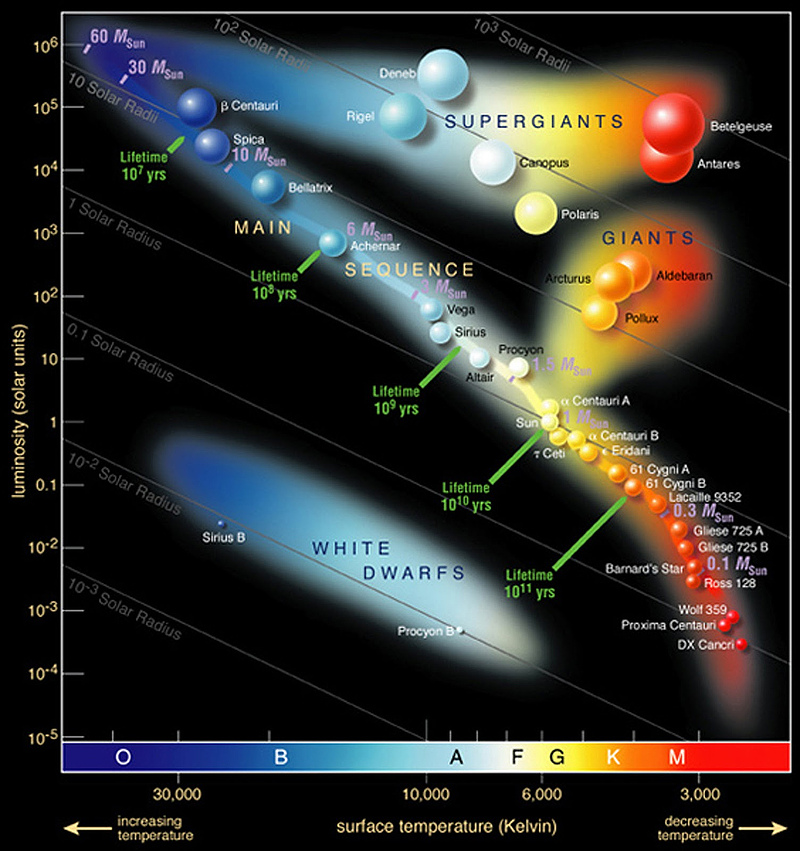
\includegraphics[width=\linewidth]{Hertzsprung-Russel_StarData}
    \caption{Hertzsprung-Russel diagram, from \url{https://www.eso.org/public/images/eso0728c/}.}
    \label{fig:hrdiagram}
\end{wrapfigure}

\subsection{Brief theory}

Stars show a large variety of luminosities and effective temperatures.
A \textsc{hr} diagram, shown in \cref{fig:hrdiagram}, is a scatter plot of stellar luminosity and effective temperature for a large sample of stars.
The location of a star in the \textsc{hr} diagram varies with the lifetime of a star during its evolution, and is mostly determined by its initial mass when it starts burning hydrogen through nuclear fusion reactions.

Stars spend most of their lifetime on the Main Sequence (the diagonal line in \cref{fig:hrdiagram}).
The specific position on the Main Sequence is determined by the mass of the star.
On the Main Sequence, stars fuse hydrogen in their cores to helium through nuclear fusion reactions.
The larger the mass of the star, the shorter the time a star spends on the Main Sequence.
Once the star runs out of hydrogen in its core, it starts burning first hydrogen in the outer core layer, and then helium in its centre, and it consequently moves from the Main Sequence to the Red Giant branch.
Eventually, stars of different masses have different fates.
Solar-like stars end their lives as white dwarfs, while heavier stars with masses larger than 8 M$_{\odot}$
explode as core-collapse supernovae.

Estimating a star's luminosity and effective temperature is not an easy task, as it involves determining the star's luminosity, while only its apparent brightness can be seen through the telescope.
The \textsc{hr} diagram is usually represented as a colour-magnitude diagram.
The absolute magnitude is a proxy for the luminosity, and the colour a proxy for the surface temperature.
Usually, the observed \textsc{hr} diagram is plotted as absolute magnitude in the V-band as a function of the B - V colour.
To estimate the absolute magnitude, one needs to know the distance to the star.
However, if all the stars that are examined are at the same distance, the absolute magnitude can be substituted by the apparent magnitude.
This happens in open clusters or globular clusters, which are concentration of stars in well defined region of space, where we can assume that each star has the same distance to the observer.

\subsection{Recommended reading}

Chapter 3 in \emph{Astrophysics for Physicists}\autocite{Choudhuri} and chapters 8.2, 10.6, 13, 15.1, 16.1, and 16.2 in \emph{An Introduction to Modern Astrophysics}\autocite{carroll2017introduction}.

\subsection{Aim of the experiment}

The aim of the experiment is to build an \textsc{hr} diagram using either open clusters or globular clusters, and to identify the different evolutionary stages of stars on the \textsc{hr} diagram.

\subsection{Observation strategy}
\begin{enumerate}
    \item Indentify suitable targets for the experiment using either lists of open clusters (e.g., \url{https://en.wikipedia.org/wiki/List_of_open_clusters}) or the Nasa Extragalactic database search feature \url{https://ned.ipac.caltech.edu/byparams}.
    \item Take calibration images (darks, flats, flat darks)
    \item Take images of the target cluster in the B and V bands.
    \item Take images of a nearby standard star for photometric calibration.
\end{enumerate}

\subsection{Data analysis}

After data acquisition, students need to perform the data reduction steps described in Section \ref{section:data_red_steps} for both the actual targets and the standard star.
The standard star is then used to measure the magnitude zero-point of each image in each band.
This produces target images that have been astrometrically and photometrically calibrated, i.e. every pixel has a specific sky position assigned and the magnitude zero-point of the image is known.

For this experiment, students need to measure the magnitudes for each star belonging to the star cluster.
They can perform these tasks using the \software{Python} packages \software{photutils} and \software{astropy}:
\begin{itemize}
    \item Perform source detection: following \url{https://photutils.readthedocs.io/en/stable/detection.html}, students need to detect and extract sources from the image.
          The provided positions of the objects are in pixel units.
    \item
          Convert pixel to sky coordinates: following
          \url{https://docs.astropy.org/en/stable/wcs/}, students need to convert the
          pixel coordinates of sources into sky coordinates, i.e.
          Right ascension (RA) and Declination (DEC) at J2000.
    \item
          Match with external catalogue: in order to know which stars belong to the star
          cluster, students need to download a reference catalogue for the star cluster
          from \url{http://vizier.u-strasbg.fr/viz-bin/VizieR} and match this catalogue
          with the detected sources via sky coordinates, following
          \url{https://docs.astropy.org/en/stable/coordinates/matchsep.html}.
    \item
          Perform photometry: students need to measure magnitudes in the B and V bands
          for each star belonging to the star cluster following
          \url{https://photutils.readthedocs.io/en/stable/psf.html}.
    \item
          Plot the HR diagram: students need to plot the HR diagram using the measured
          magnitudes and identify the different evolutionary stages on it.
          If the single star cluster contains few stars, then different star clusters stars may be put on the same plot, provided that their absolute magnitude has been estimated.
\end{itemize}

Similar steps need to be performed on the standard star image in order to measure its instrumental magnitude and therefore the magnitude zero-point of the image.

\section{Period-Luminosity relation of Cepheids}

\subsection{Brief theory}

Cepheids are a class of pulsating stars that vary their luminosity in a periodic way.
The luminosity of these objects depends only on the size and composition (metallicity) of the star.
These stars are not located on the Main Sequence of stars of the Hertzsprung-Russell (HR) diagram.
Indeed, they oscillate between the Main sequence and the instability strip (Figure \cref{fig:cepheid-lightcurve}).
Being Cepheids rare, their pulsation is a transient phenomenon.

Several mechanisms can produce stellar pulsations.
In short, the Cepheid acts like a gigantic heat engine of which the volume and pressure change in time similarly to a thermodynamic cycle.
Since the oscillation period depends only on the properties of the star such as its mass and composition, once we know composition (through spectroscopy) and period of oscillation, we can deduce its luminosity.
As a matter of fact, for most Cepheids there is a very specific relationship between their period and their absolute magnitude, the so-called period-luminosity relation.
This relation has been empirically calibrated in different wavebands by astronomers.
By measuring the period of the star and by then measuring its brightness, one can deduce the distance to the star.
Cepheids are indeed called standard candles.

\begin{figure}
    \centering
    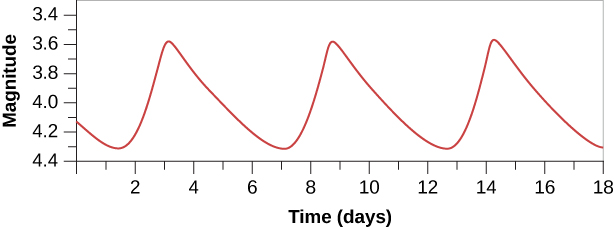
\includegraphics[width=0.7 \textwidth]{cepheid-light-curve}
    \caption{The lightcurve of a Cepheid has a period that depends on its absolute magnitude. %From \url{https://phys.libretexts.org/Bookshelves/Astronomy__Cosmology/Book%3A_Astronomy_(OpenStax)/19%3A_Celestial_Distances/19.03%3A_Variable_Stars-_One_Key_to_Cosmic_Distances}.}
    }
    \label{fig:cepheid-lightcurve}
\end{figure}

Further references students need to read are chapter 2.2.7 in [3] and chapter 8.2, 10.6, 13, 14 in \emph{An Introduction to Modern Astrophysics}\autocite{carroll2017introduction}.

\subsection{Aim of the experiment}

The aim of the experiment is to estimate the distance to the Cepheid stars using the calibrated period-luminosity relation in the V-band.
Students need to identify suitable targets for the experiment using e.g., the Nasa Extragalactic database search feature \url{https://ned.ipac.caltech.edu/byparams}.
During the observations, students need to collect the calibration images (bias, dark, flat) and images of their targets in the V-band.
Students need also to collect images of a standard star to estimate the photometric zero-point.
Students need to create the light curve of Cepheid variables, therefore multiple nights of observations are required for this experiment.
Once data are collected, students perform a data reduction and data analysis to estimate the period from the light curve and then the distance to the star through the period-luminosity relation.

\subsection{Data Analysis steps}

After data acquisition, students need to perform the data reduction steps described in Section \ref{section:data_red_steps} for both the actual targets and the standard star.
The standard star is then used to measure the magnitude zero-point of each image in each band.
This produces target images that have been astrometrically and photometrically calibrated, i.e. every pixel has a specific sky position assigned and the magnitude zero-point of the image is known.

For this experiment, students need to measure the magnitudes as a function of time (epochs) for each Cepheid star.
They can perform these tasks using the \software{Python} packages `photutils' and `\software{astropy}':
\begin{itemize}
    \item Perform source detection: following \url{https://photutils.readthedocs.io/en/stable/detection.html}, students need to detect and extract sources from the image.
          The provided positions of the objects are in pixel units.
    \item
          Perform photometry: students need to measure the Cepheid magnitudes in V-band
          for the multiple epochs following
          \url{https://photutils.readthedocs.io/en/stable/psf.html}.
    \item
          Period: students need to plot the light curve of Cepheids and measure their
          pulsation period.
    \item
          Distance: using the calibrated period-luminosity relation in the V-band,
          students need to measure the distance to each Cepheid variable.
\end{itemize}

Similar steps need to be performed on the standard star image in order to measure its instrumental magnitude and therefore the magnitude zero-point of the image.

\section{Star-formation rate of galaxies with the Hα line}

\subsection{Brief theory}

Different kind of galaxies produce stars at different rates during the course of their lifetime.
The amount of stars produced by galaxies is generally defined as star-formation rate (SFR) and it indicates the amount of stars in units of solar masses produced per year.
Elliptical galaxies generally have a low SFR, while spiral galaxies a higher one.
Star-formation occurs in the dense regions of molecular clouds, i.e. regions where molecular hydrogen is available.
When stars ignite their hydrogen burning in the core, they emit a large number of ionizing photons that ionize the sorrounding medium giving rise to the so-called HII regions (Figure \ref{fig:hiiregions}).

\begin{figure}[t!]
    \centering
    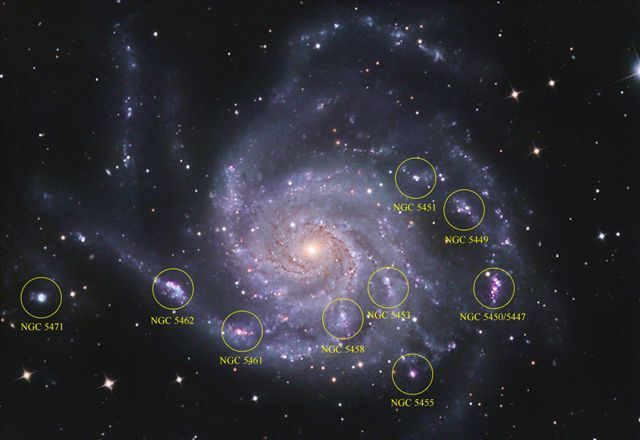
\includegraphics[width=12cm]{m101.jpg}
    \caption{M101 and its HII regions of ongoing star-formation.
        Credits to George Golitzin (\url{https://www.cloudynights.com/topic/333679-hii-regions-in-m101/}).
    }
    \label{fig:hiiregions}
\end{figure}

An indicator for the ongoing star-formation in galaxies is the Hα luminosity.
During the formation of stars, especially heavy ones, a great amount of ionizing photons is produced.
These can ionize the surrounding hydrogen gas.
When the protons and electrons recombine, they might recombine into an exited state instead of into the hydrogen ground state.
By emitting photons, these exited states can fall back to the ground state.
The Hα line corresponds to the n=3 to n=2 transition in the Balmer series and it emits a photon at a wavelength of 656.28 nm.
By measuring the Hα luminosities in galaxies and using the calibrated relations between luminosities and star-formation rates, we can measure the ongoing SFR in galaxies in units of solar masses per year.

Further references students need to read for the experiment are chapters 6.6, 6.6.4, 9.1,9.2 in \emph{Astrophysics for Physicists}\autocite{Choudhuri}, chapter 25 in \emph{An Introduction to Modern Astrophysics}\autocite{carroll2017introduction}, chapters 3.1, 3.3.1, 3.3.2, 3.9.4, 3.9.5 in [3], \url{https://ned.ipac.caltech.edu/level5/Sept12/Calzetti/Calzetti1_2.html} and \url{https://ned.ipac.caltech.edu/level5/Sept01/Rosa/frames.html}

\subsection{Aim of the experiment}

The aim of the experiment is to measure the SFR of a sample of local spiral galaxies using the Hα line.
Students need to identify suitable targets for the experiment using e.g., the Nasa Extragalactic database search feature \url{https://ned.ipac.caltech.edu/byparams}.
During the observations, students need to collect the calibration images (bias, dark, flat) and images of their targets in the Hα-band.
Students need also to collect images of a standard star to estimate the photometric zero-point.
Once data are collected, students perform a data reduction and data analysis to measure the flux from the HII regions, convert it into luminosities using the distance to the object and then measure the SFR using the empirical relation between luminosity in Hα and SFR.

\subsection{Data Analysis steps}

After data acquisition, students need to perform the data reduction steps described in Section \ref{section:data_red_steps} for both the actual targets and the standard star.
The standard star is then used to measure the magnitude zero-point of each image in each band.
This produces target images that have been astrometrically and photometrically calibrated, i.e. every pixel has a specific sky position assigned and the magnitude zero-point of the image is known.

For this experiment, students need to measure the flux from HII regions in the spiral galaxies.
They can perform these tasks using the \software{Python} packages `photutils' and `\software{astropy}':
\begin{itemize}
    \item Perform source detection: following \url{https://photutils.readthedocs.io/en/stable/detection.html}, students need to detect and extract sources from the image.
          The provided positions of the objects are in pixel units.
    \item
          Perform photometry: students need to measure the flux from HII regions in the
          Hα-band following
          \url{https://photutils.readthedocs.io/en/stable/aperture.html}.
    \item
          Estimate luminosity: students need to measure Hα luminosities using fluxes and
          distances from galaxies.
    \item
          Star-formation rate: using the calibrated relation between luminosity and
          star-formation rate, students need to measure the latter and compare it to
          literature values.
\end{itemize}

Similar steps to those highlighted in Section 7.1.3 need to be performed on the standard star image in order to measure its instrumental magnitude and therefore the magnitude zero-point of the image.

\section{Galaxy morphology with \software{GALFIT}}

\subsection{Brief theory}

Galaxies in the Universe show a wide range of morphologies.
They range from spheroidal aggregation of stars such as elliptical galaxies to disk objects with spiral arms such as spiral galaxies to irregularly shaped galaxies resulting from interactions or feedback from the interstellar medium.
One of the very first morphological classification of galaxies was performed by Edwin Hubble in its famous tuning-fork diagram (Figure \ref{fig:tuningfork}).

\begin{figure}
    \centering
    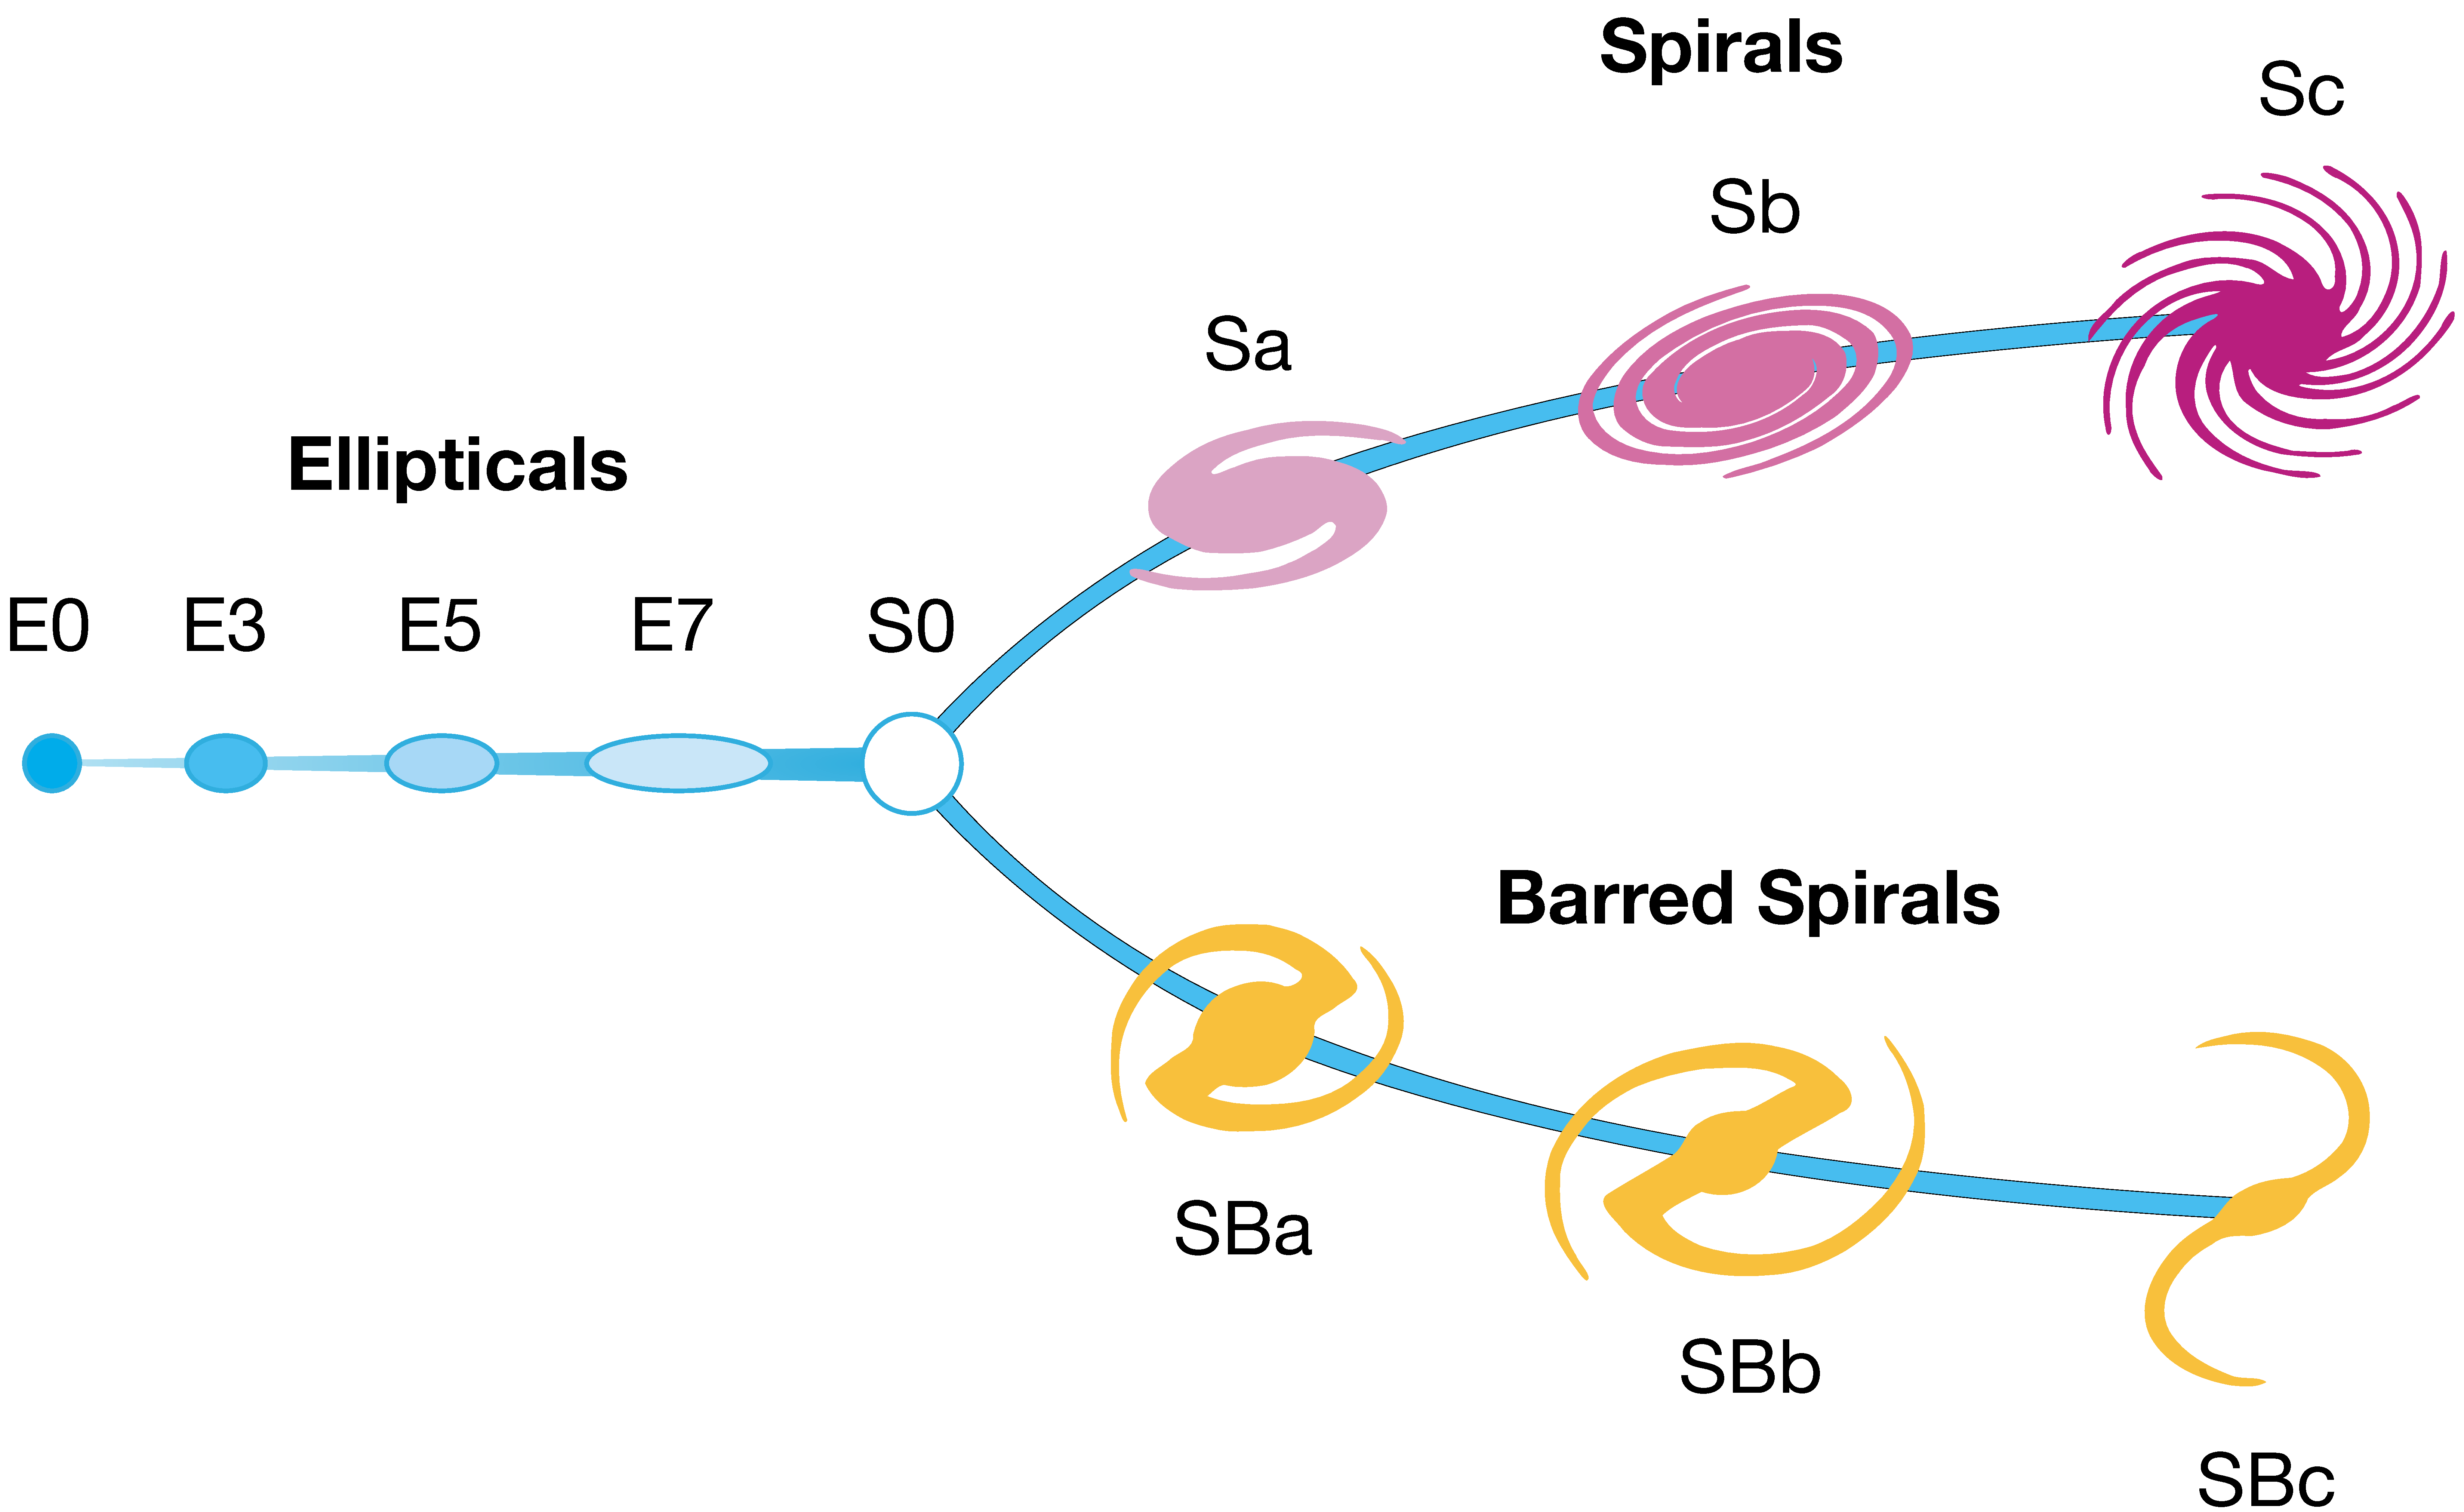
\includegraphics[width=0.7\textwidth]{tuningfork}
    \caption{Hubble tuning-fork diagram.}
    \label{fig:tuningfork}
\end{figure}

The visual morphological classification of galaxies is a task that requires a lot of experience and expertise.
Even professional astronomers may find difficult to classify a galaxy, especially if the galaxy is far away and the resolution of the telescope is poor.
An alternative way of morphologically classify a galaxy is by looking at its light distribution, i.e. the intensity of light as a function of the galaxy radius.
The most general light profile distribution is the S\'ersic light profile (S\'ersic 1963) where the intensity of light scales as I(R)
$\propto$e$^{\mathrm{-b R^{1/n}}}$, with n being the S\'ersic index.
n is usually equal to $\sim$ 4 for elliptical galaxies and $\sim$ 1 for spiral galaxies.
Different softwares are available to measure the galaxy light profile.
One of the more robust ones is \software{GALFIT} (Peng et al.
2010) that is a two-dimensional fitting algorithm designed to extract
structural components from galaxy images.

Further references students need to read for the experiment are chapters 9.1,9.2 in \emph{Astrophysics for Physicists}\autocite{Choudhuri}, chapter 25 in \emph{An Introduction to Modern Astrophysics}\autocite{carroll2017introduction}, chapters 3.1, 3.2.1, 3.2.2, 3.2.3, 3.3.1, 3.3.2 in [3], \software{GALFIT} manual and \url{https://ned.ipac.caltech.edu/level5/Sept11/Buta/frames.html}.

\subsection{Aim of the experiment}

The aim of the experiment is to morphologically classify a sample of local elliptical and spiral galaxies using the software \software{GALFIT}.
Students need to identify suitable targets for the experiment using e.g., the Nasa Extragalactic database search feature \url{https://ned.ipac.caltech.edu/byparams}.
During the observations, students need to collect the calibration images (bias, dark, flat) and images of their targets in the B, V and R bands.
Students need also to collect images of a standard star to estimate the photometric zero-point.
Once data are collected, students perform a data reduction and data analysis to fit the galaxy light profiles with \software{GALFIT} and estimate the best-fitting total magnitude, half-light radius and S\'ersic index.
On the base of the S\'ersic index value, students need to classify their galaxies and compare their classification with the literature one.

\subsection{Data Analysis steps}

After data acquisition, students need to perform the data reduction steps described in Section \ref{section:data_red_steps} for both the actual targets and the standard star.
The standard star is then used to measure the magnitude zero-point of each image in each band.
This produces target images that have been astrometrically and photometrically calibrated, i.e. every pixel has a specific sky position assigned and the magnitude zero-point of the image is known.

For this experiment, students need to use \software{GALFIT} to fit the galaxy image with a S\'ersic light profile following the examples in \url{https://users.obs.carnegiescience.edu/peng/work/GALFIT/GALFIT-ex.tar.gz} and the rules of thumb in \url{https://users.obs.carnegiescience.edu/peng/work/GALFIT/TOP10.html}.
Students also needs to use `photutils' and `\software{astropy}' for specific tasks.
\begin{itemize}
    \item
          Data reduction: images need to be photometrically and astrometrically
          calibrated.
    \item
          Model of the PSF: \software{GALFIT} convolves the light profile with the
          point-spread function (PSF) of the telescope+detector, therefore a model image
          of the PSF needs to be created.
          Students can follow \url{https://photutils.readthedocs.io/en/stable/epsf.html#build-epsf} to build a model of the PSF.
    \item
          Initial guess: an initial guess for the parameters of the S\'ersic model needs
          to be provided to \software{GALFIT}.
          One example is to measure the magnitude and half-light radius in an elliptical aperture following \url{https://photutils.readthedocs.io/en/stable/isophote.html}.
          An initial guess of n=2.5 is good enough for our purposes.
    \item
          galaxy fitting: students perform a galaxy image fitting with \software{GALFIT}.
          They need to report the best-fitting parameters, together with the model and the residual images.
          A morphological classification needs to be performed according to the best-fitting S\'ersic index value.
\end{itemize}

Similar steps to those highlighted in Section 7.1.3 need to be performed on the standard star image in order to measure its instrumental magnitude and therefore the magnitude zero-point of the image.

\begin{figure}[t!]
    \centering
    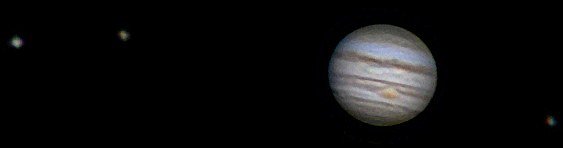
\includegraphics[width=12cm]{jupiter}
    \caption{Jupiter and its moons from an amateur telescope.
        Credits to Thomas Bresson and Rochus Hess.
    }
    \label{fig:jupyter}
\end{figure}

\section{Mass of Jupiter and Saturn}

\subsection{Brief theory}

The two largest planets of the Solar System, Saturn and Jupiter, are also the ones having the largest number of moons.
By inspecting their orbital motion, it is possible to estimate the mass of these two gas giants.
If we assume that the moons move on circular orbits around Jupiter and Saturn and if we assume that their mass is negligible with respect to the planet, then we can equate Newton's law
\begin{equation}
    F_G = G \frac{m_1 m_2}{r^2}
\end{equation}
where $G$ is the gravitational constant,
$m_1$ and $m_2$ the mass of the attracting bodies,
r the distance between the two bodies, with the centripetal force
\begin{equation}
    F_C = m \omega^2 r
\end{equation}
where
$m$ is the mass of the moving object,
$\omega$ its angular velocity and
$r$ the distance from the centre of its orbit.
By equating them and using the relation between angular velocity and period for circular orbit we obtain
\begin{equation}
    \frac{T^2}{r^3} = \frac{4 \pi^2 G}{M}
\end{equation}
where $M$ is the mass of Jupiter or Saturn.

Further reference students need to read for the experiment is chapter 21 in \emph{An Introduction to Modern Astrophysics}\autocite{carroll2017introduction}.

\subsection{Aim of the experiment}

The aim of the experiment is to measure the mass of Jupiter and/or Saturn using their moon orbits \ref{fig:jupyter}.
This experiment is not always available given the different relative positions of Sun, Earth and Jupiter/Saturn during the years.
During the observations, students need to collect the calibration images (bias, dark, flat) and images of their targets in the B, V and R bands.
Students need also to collect images of a standard star to estimate the photometric zero-point.
They need to take multi-epoch observations of Jupiter/Saturn and their moons in order to reconstruct the orbit of the objects.
Multiple days of observations are therefore required to obtain optimal results.
Students need to perform a data reduction and analyse the data to estimate Jupiter/Saturn mass.

\subsection{Data Analysis steps}

After data acquisition, students need to perform the data reduction steps described in Section \ref{section:data_red_steps} for both the actual targets and the standard star.
The standard star is then used to measure the magnitude zero-point of each image in each band.
This produces target images that have been astrometrically and photometrically calibrated, i.e. every pixel has a specific sky position assigned and the magnitude zero-point of the image is known.

For this experiment, students need to measure the relative distances between the moons and the planet as a function of time.
They can perform these tasks using the \software{Python} packages `photutils' and `\software{astropy}':
\begin{itemize}
    \item Perform source detection: following \url{https://photutils.readthedocs.io/en/stable/detection.html}, students need to detect and extract sources from the image.
          The provided positions of the objects are in pixel units.
    \item
          Convert in absolute distances: by using simple trigonometry, students need
          first to convert the distance in pixel between sources in angular distance
          (using the pixel scale) and then in absolute distance in meters by using the
          Earth-Jupiter distance at the time of observation.
    \item
          Plot the distance: students need to plot the obtained distances as a function
          of time and, assuming a circular motion, compute the period, amplitude and
          phase of the orbital motion of the moons.
          They can use the \software{scipy} curve\_fit function to fit the curve to the data.
    \item
          Compute the mass: using the best-fitting period, students need to derive the
          mass of Jupiter/Saturn together with the error on this estimate.
\end{itemize}

\section{Planetary Albedo}

\subsection{Brief Theory}
\label{subsection:albedo_theory}

Planets do not emit significant light through nuclear reactions as the Sun does.
They have other physical processes that emit light, but the amount of radiation is too small to make them visible from Earth.
Planets absorb and reflect light from the Sun and this latter effect makes them visible from Earth.
The amount of radiation that a planet reflects is called `albedo'.
The albedo depends on the characteristics of its surface and atmosphere.
For example, a planet covered in ice is going to reflect a lot more light than a planet with a rocky surface.
Calculating this quantity with empirical data can therefore help us get some information about the composition of the planet outer shell.
The ratio between the incoming $L_\text{in}$ and reflected radiation $L_\mathrm{out}$ from a planet is given by:
\begin{equation}
    A = \frac{L_\text{out}}{L_\text{in}} = p \cdot q
\end{equation}
where
$p$ and $q$ are the geometric albedo and the phase integral, respectively.
$p$ gives information about the intrinsic properties of the planet,
$q$ includes the phase angle dependence.
$p$ has a value between $0$ (absorbs all radiation) and $1$ (reflects all radiation).
The formula to compute the geometric albedo is
\begin{equation}
    p = \left ( \frac{r \Delta}{a R} \right) \cdot 10^{-0.4(m - m_{\odot})}
\end{equation}
where $\Delta$ is the distance Earth-planet,
$a$ is the Sun-Earth distance in AU,
$r$ is the planet-Sun distance,
$R$ the planet radius,
$m$ is the planet apparent magnitude and m
$_{\odot}$ is the Sun apparent magnitude.

Further reference the students have to read is chapter 7 in [4].

\subsection{Aim of the experiment}

The aim of the experiment is to measure the geometric albedo of the Solar system planets.
The targets for the experiment depends on which planets are observable from Earth in the specific semester of observations.
During the observations, students need to collect the calibration images (bias, dark, flat) and images of their targets in the B, V and R bands.
Students need also to collect images of a standard star to estimate the photometric zero-point.
They then measure the calibrated apparent magnitudes and the geometric albedos in the B, V and R bands.

\subsection{Data Analysis steps}

After data acquisition, students need to perform the data reduction steps described in Section \ref{section:data_red_steps} for both the actual targets and the standard star.
The standard star is then used to measure the magnitude zero-point of each image in each band.
This produces target images that have been astrometrically and photometrically calibrated, i.e. every pixel has a specific sky position assigned and the magnitude zero-point of the image is known.

For this experiment, students need to measure the albedos of planets.
They can perform these tasks using the \software{Python} package `photutils':
\begin{itemize}
    \item Perform photometry: students need to measure the background subtracted fluxes from the planets following \url{https://photutils.readthedocs.io/en/stable/aperture.html}.
          Then they can translate that into magnitudes using the photometric zero-point estimated from the standard star.
    \item
          Estimate the geometric albedo: using the formula in section
          \ref{subsection:albedo_theory}, students need to measure the geometric albedo
          and its error and compare it to literature values.
          The values for the apparent magnitude of the sun, the distance of the planet from Earth and Sun can be easily found in literature.
\end{itemize}

\subsection{References}

[3] Extragalactic Astronomy and Cosmology, Peter Schneider, Springer

    [4] Fundamental Astronomy, Hannu Karttunen, Springer

\chapter{Planning observations}

\section{Picking targets}

E.g. in Stellarium, N.I.N.A Sky Atlas, other database .
..

Good properties:

Fulfills science requirements (see experiments section)

High surface brightness or total brightness (TODO figure approx.
sensitivity/magnitude limit)

High above the horizon (to avoid light pollution)

Not covered by the building

Small enough to fit on the sensor

Large enough to be resolved sufficiently

Visible during astronomical darkness, ideally for the next months

Far away from the moon, if visible (Changes all the time)

\section{Setting exposure parameters}

There are several parameters that you can choose when taking exposures of targets: filter, exposure time, number of exposures, binning, dithering etc. The goal of this section is to help you choose the correct settings.

Know all the noise levels

The zero level of the detector is around 1000 ADUs, with a sigma of about 9.

For L filter, at Zenith, you get about 200 ADUs over 30 seconds of sky background, or 6.6 ADU/s.

This corresponds to about 10 electrons per second, which is 10 photons per second, per pixel.

\backmatter

\appendix \addcontentsline{toc}{part}{Appendices}

\chapter{List of Standard Stars}

\begin{figure}
    \centering 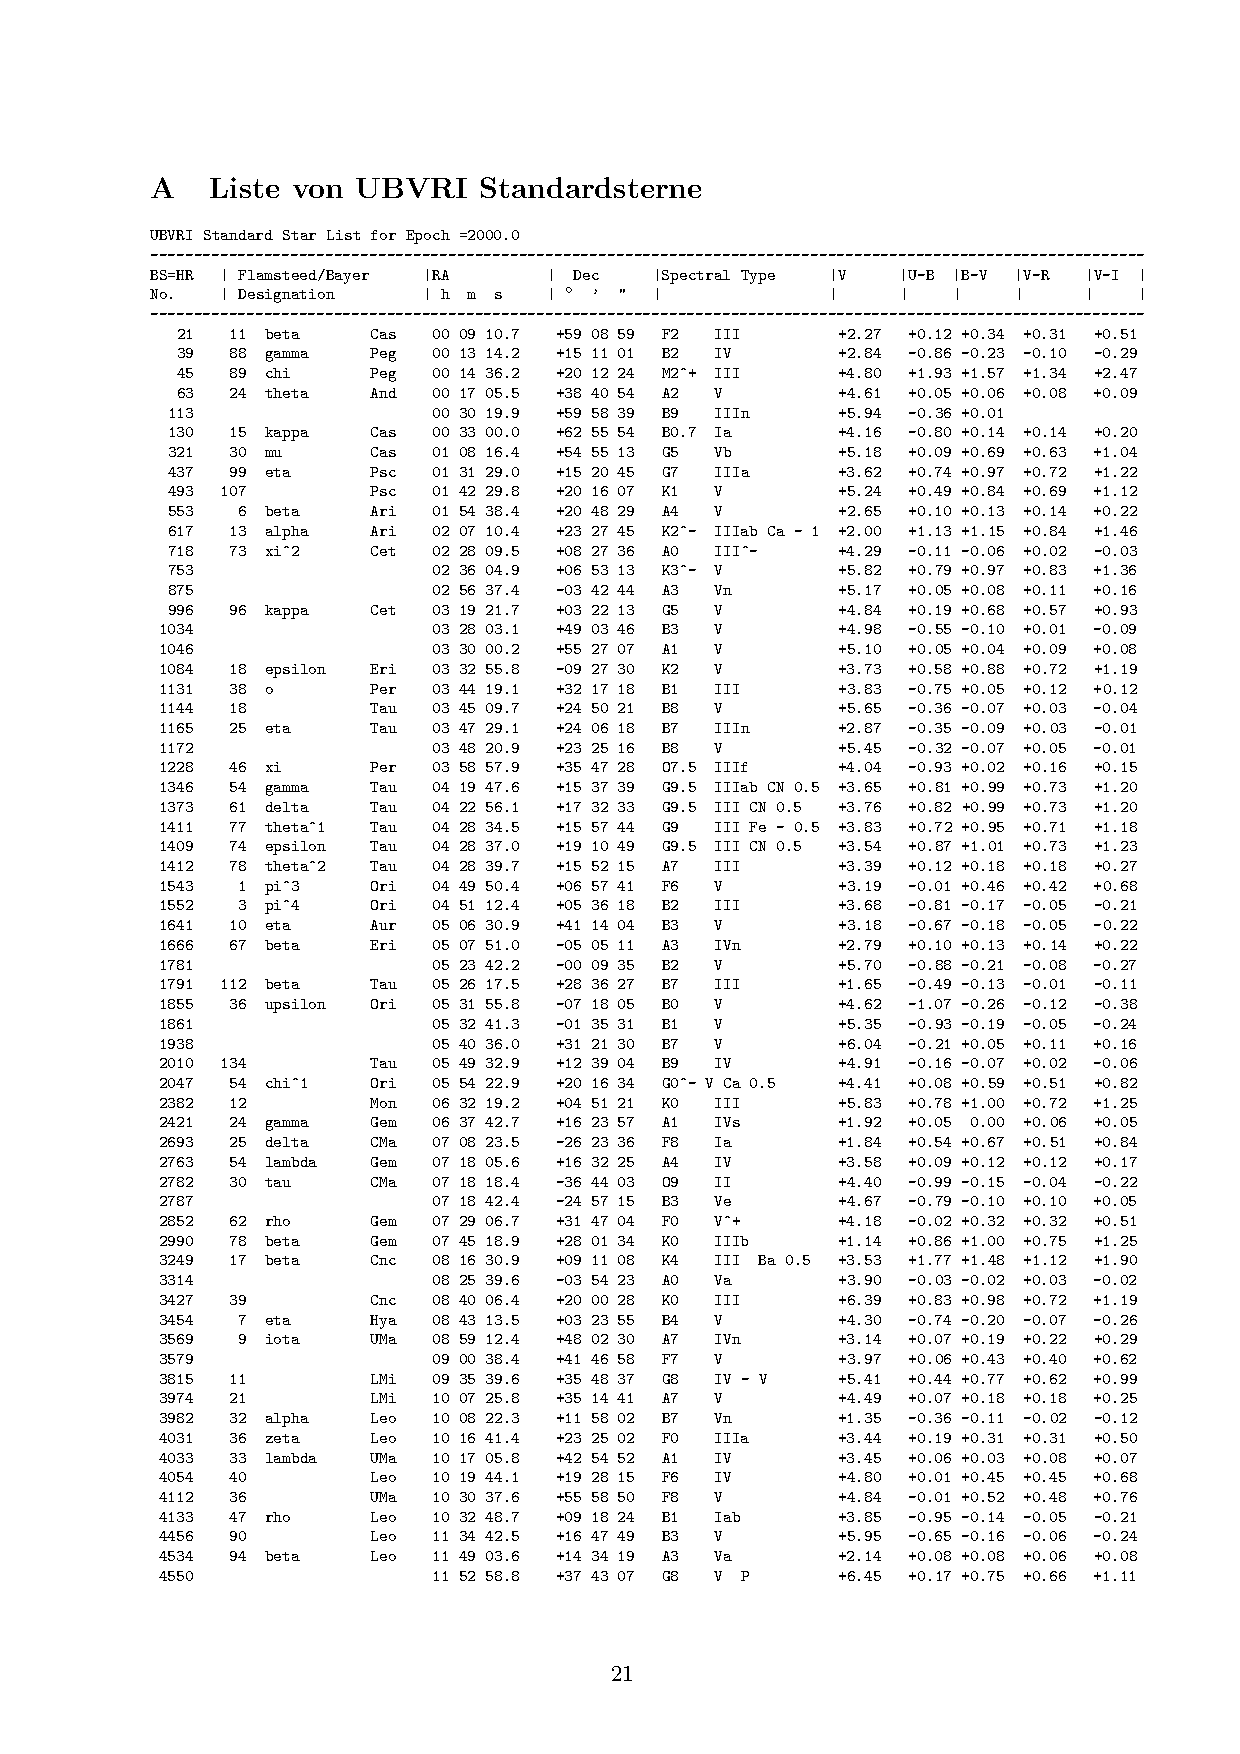
\includegraphics[width=14cm]{standardsterne_ubvri1} \caption*{} \label{}
\end{figure}

\begin{figure}
    \centering \includegraphics[width=14cm]{standardsterne_ubvri2} \caption*{} \label{}
\end{figure}

\chapter{Administrative Notes}

This document describes the administrative preparations (observatory access, computing access) for the advanced student lab (ASL).

\subsection{Registration}
The \textsc{asl} is part of the \textsc{vp}, and as for all \textsc{vp} experiments, the students have to sign up for the experiment at room \textsc{hpp} \textsc{h} 12.
After registration, the students will contact (or will be contacted by) the observatory supervisor for an introduction to the observatory and the experiments.

Because of the strong weather dependence of the observations, the number of students per semester is limited, and the registration is valid for the entire semester.
Admission is first-come, first-served at \textsc{hpp} \textsc{h} 12.

\subsection{Access to the building}
The \textsc{hpp} building is generally open during weekdays, as can be confirmed on the website of the building.
If you want to access the building outside the regular opening hours, i.e. at night or on weekends, you have to apply for access rights with your \textsc{eth}-card (\enquote{Legi}).
You can ask the secretary of the group that is in charge of the \textsc{hpp} observatory for access rights.

If you have access rights to the \textsc{hpp} building, you can use your \textsc{eth}-card at the card terminal at the front door to access the building: Simply hold the card close to the scanner, enter your password, and press enter.
If this is the first time you are using this system, you have to set your password online\footnote{\url{www.bi.id.ethz.ch/eAdressen/index_en.jsp}} beforehand.

\subsection{Access to the observatory}
Two keys are required to access all the facilities of the observatory.
The keys can either be borrowed on a per-night basis from the supervisor of the observatory, or they can be organized by the secretary of the group in charge of the \textsc{hpp} observatory if frequent access is required.

\printbibliography

\end{document}
